%% This document gives an example on how to use the ntnumasterthesis
%% LaTeX document class.

%% Use short name MACS, MIS, CIMET, MTDMT, MIXD or MIS  
%% Language english or norsk
%% b5paper with oneside or twoside, you can set A4 if you want but you submit in b5

%% If you want print with the heading material on a4 paper you can use this format
%% \documentclass[MACS,en glish,a4paper,oneside,12pt]{ntnuthesis/ntnuthesis}

%% with the change to using DAIM we have a new option. include DAIM after english below removes the front page material so that you can then submit in the DAIM system. If you are wanting the front material remove DAIM and make sure you fill in the DaimData.tex file.
\documentclass{report}
%[MACS,english]{ntnuthesis/ntnuthesis
\renewcommand{\baselinestretch}{1.2} 

\usepackage[T1]{fontenc}
\usepackage[utf8]{inputenc}     % For utf8 encoded .tex files allows norwegian characters in the files. This can be dangerous if you change to a differnt editor.
%\usepackage[pdftex]{graphicx, hyperref}   % For cross references in pdf
\usepackage{graphicx}
\usepackage{hyperref}   % For cross references in pdf

% For smart references 
%    use \cref{label} and Caption and Number will be added automatically
\usepackage[capitalise,noabbrev]{cleveref} 
\usepackage[nottoc]{tocbibind}
\usepackage{url}
\usepackage{color}              % For colouring text 
\hypersetup{colorlinks=true,     
		linkcolor=black,          % color of internal links (change box color with linkbordercolor)
    citecolor=blue,        % color of links to bibliography
    filecolor=black,      % color of file links
    urlcolor=black           % color of external links
		}
\usepackage{csvsimple}  % for simple table reading and display
\usepackage{url}
\usepackage{booktabs}
\usepackage{gnuplottex} %miktex option if using miktex on windows
\usepackage{rotating}
\usepackage{gensymb}
\usepackage{float}
\usepackage[utf8]{inputenc}
\usepackage{enumitem}
\usepackage{multirow}
\usepackage{amssymb}
\usepackage{amsmath}
\usepackage{tocloft}
\usepackage{float}
\usepackage{appendix}
\renewcommand*\contentsname{Contents}
\usepackage{array}
\usepackage{subfig}
\usepackage{color}
\usepackage{gensymb}
\usepackage{multicol}
\usepackage{listings}
\usepackage{varwidth}
\usepackage{enumitem}
\usepackage{chngcntr}
\usepackage{fancyhdr}
\counterwithin{figure}{section}
\usepackage{vmargin}
\usepackage{datetime}
\usepackage{pdfpages} 
%\usepackage{fourier}

\usepackage{todonotes}
\usepackage{sectsty}



\pagenumbering{roman}

\setmarginsrb{3 cm}{2.5 cm}{3 cm}{2.5 cm}{1 cm}{1.5 cm}{1 cm}{1.5 cm}
\pagestyle{fancy}
\fancyhf{}
\rhead{\theauthor}
\lhead{\thetitle}
\cfoot{\thepage}


\pagestyle{fancy}
\fancyhf{}
\rhead{\theauthor}
\lhead{\thetitle}
\cfoot{\thepage}
\title{Identification of plastics using Hyperspectral Imaging}								% Title
\author{Emilie M. Hyrum Dahl}								% Author
\date{Fall 2018}											% Date

\makeatletter
\let\thetitle\@title
\let\theauthor\@author
\let\thedate\@date
\makeatother


\definecolor{darkgreen}{rgb}{0,0.5,0}
\definecolor{darkred}{rgb}{0.5,0.0,0}

\lstset{        basicstyle=\ttfamily,
                keywordstyle=\color{blue}\ttfamily,
                stringstyle=\color{darkred}\ttfamily,
                commentstyle=\color{darkgreen}\ttfamily,
}

\usepackage{vmargin}
\setmarginsrb{2 cm}{2.5 cm}{2 cm}{2.5 cm}{1 cm}{1.5 cm}{1 cm}{1.5 cm}

%Typesetting of C++ but not always stable in titles etc...
\newcommand{\CPP}[0]{{C\nolinebreak[4]\hspace{-.1em}\raisebox{.1ex}{\small\bf +\hspace{-.1em}+\ }}}

%\usepackage[table]{xcolor}% http://ctan.org/pkg/xcolor
%\usepackage[nomessages]{fp}
%\newlength{\maxbarlen}


\newcommand\databar[3][gray!20]{%
  \FPeval\result{round(#3/#2:4)}%
  \rlap{\textcolor{#1}{\hspace*{\dimexpr-\tabcolsep+.5\arrayrulewidth}%
        \rule[-.05\ht\strutbox]{\result\maxbarlen}{.95\ht\strutbox}}}%
  \makebox[\dimexpr\maxbarlen-2\tabcolsep+\arrayrulewidth][r]{#3}}



\newcommand{\com}[1]{{\color{red}#1}} % supervisor comment
%\renewcommand{\com}[1]{} %remove starting % to remove supervisor comments
% This will appear in text \com{Lecuters comment} and be visible unless you uncomment
% the renewcommand line.

\newcommand{\todo}[1]{{\color{green}#1}} % items to do
%\renewcommand{\todo}[1]{} %remove starting % to remove items to do

\newcommand{\n}[1]{{\color{black}#1}} % other comment
%\renewcommand{\n}[1]{} %remove starting % to remove notes

\newcommand{\dn}[1]{} % add the d to a note to say that you have finished with it.





% Set to true ONLY if using Harvard citation style
\newboolean{HarvardCitations}
\setboolean{HarvardCitations}{true} % false for computer science, true for interaction design and harvard style


\ifthenelse{\boolean{HarvardCitations}}{%
	\usepackage{natbib} % for Harvard names as citations.
}{%
	\usepackage[numbers]{natbib} % for Vancover numbers in bibliography
}

%\newcommand{\q}[1]{\leavevmode\marginpar{\small\em #1}}
%\renewcommand{\q}[1]{}


\usepackage{nomencl}
\makenomenclature
 
%% This code creates the groups
% -----------------------------------------
\usepackage{etoolbox}
\renewcommand\nomgroup[1]{%
  \item[\bfseries
  \ifstrequal{#1}{RL}{Roman Letters}{%
  \ifstrequal{#1}{MV}{Matrices and Vectors}{%
    \ifstrequal{#1}{GL}{Greek Letters}{%
  \ifstrequal{#1}{AB}{Abbrevations}{}}}}%
  
]}

\begin{document}

\begin{titlepage}
	\centering
    \vspace*{0.5 cm}
    
\includegraphics[scale = 0.3]{figures/ntnuu}\\[1.0 cm]	% University Logo
    \begin{centering}
    \textsc{\LARGE Norwegian University of \newline\newline Science and Technology}\\[1.0 cm]	% University Name
    \end{centering}
	%\textsc{\Large Emilie Dahl}\\[0.5 cm]				% Course Code
	\rule{\linewidth}{0.3 mm} \\[0.4 cm]
	{ \huge \bfseries \thetitle}\\
	\rule{\linewidth}{0.3 mm} \\[1.3 cm]
	
	\begin{minipage}{0.4\textwidth}
		\begin{flushleft} \large
			\emph{Author:} \\
	    	Emilie M. Hyrum Dahl
			\end{flushleft}
			\end{minipage}~
			\begin{minipage}{0.4\textwidth}
            
			\begin{flushright} \large
	        \emph{Supervisor:}\\
			Professor Asgeir J. S{\o}rensen\\
		\end{flushright}
		\end{minipage}\\[0.5 cm]
		
		
			\begin{minipage}{0.8\textwidth}
			\begin{flushright} \large
			\emph{Co-supervisors:}\\
			Professor Geir Johnsen\\
			Aksel Alstad Mogstad
			\end{flushright}
		
        
	\end{minipage}\\[2 cm]
	
\end{titlepage}

%\input{inc/DaimData} % this is the file which contains all the details about your thesis
%\makefrontpages % make the frontpages
%this is the intro to the thesis
%\thesistitlepage % make the ordinary titlepage
\hypersetup{pageanchor=true}
%\chapter*{Summary}

\chapter*{Preface}
This thesis is submitted in partial fulfillment of the requirements for the degree of master of science (MSc) at the Norwegian University of Science and Technology (NTNU). The main work is conducted at Department of Marine Technology, NTNU, while part of the work has been conducted at Trondheim Biological Station, NTNU in cooperation with Aksel Alstad Mogstad, Department of Biology, and Geir Johnsen, Department of Biology. 
\\\\
Throughout this project, I have cooperated with Andreas {\O}. R. Stien in large part. Next to all testing and experimental work done, have been conducted together with Andreas. We therefore find it appropriate to share chapters directly connected to the experiment. The chapters \textit{Method} and \textit{Results and Discussion} in this delivery are more or less similar to the associated sections in Andreas’ delivery. In addition, Andreas and I will work together for the masters thesis starting next year. The chapter regarding conclusions and further work is therefore, more or less, equally written. 
\\\\
The work supporting this thesis is three-folded. In order to achieve relevant and precise knowledge, a study of relevant literature was conducted. This study include research on both specific methods and technology used, and what has been done in general. The research regarding these topics were done mainly through studying a set of scientific papers. However, even with the most recent publications, there are still research done - not yet published. The second part of this thesis was therefore to travel around Trondheim meeting with the experts. During exciting meetings with Emlyn Davies, Andy M. Booth, Geir Johnsen, Aksel Alstad Mogstad, Bert van Bavel, Asgeir J. S{\o}rensen and Albert Van Oyen - from now on referred to as \textit{the experts} - new knowledge was acquired. After this, the problem description finally took form. Through planning with the experts, the experiment description were formed. These experiments represent the third and last part of the three-folded work. 
\\\\
This semester, I have had two very relevant module courses, \textit{TTK19 Structures and Contexts in Complex Systems} -  a course on how to handle Quantitative Big Data, and \textit{TTK20 Hyperspectral remote sensing} - describing the hyperspectral imaging process. Throughout these courses, I have gained much relevant knowledge, some reflected in this thesis.


\begin{comment}
\newline
\newline

\newline
\newline
\newline
\newline
\newline
\newline
\begin{center}
    Trondheim, November 14, 2018
    \end{center}
\begin{figure}[H]
\centering
%\includegraphics[scale=0.5]{figures/sign}
\end{figure}
\begin{center}
Emilie Dahl
\end{center}
\end{comment}

\chapter*{Acknowledgment}
This project thesis and final report has been supported by members of the faculty at NTNU. The author of this report would particularly like to thank supervisor Professor Asgeir J. S{\o}rensen at IMT NTNU and PhD. candidate Aksel Alstad Mogstad, who have been at close guidance throughout this project and the entire semester. 
\\\\
In addition, a great thanks should be directed towards Professor Geir Johnsen at the Department of Biology NTNU, who provided insight and expertise that greatly assisted the project and thereby this report. \todo[inline, color=orange!30]{skal jeg ta med hele lista her?}



\include{Abstract}


%\includepdf[pages=-]{inc/description} 
%\setboolean{@twoside}{false}
%\includepdf[pages=-, offset=75 -75]{inc/description.pdf}
%\thesistitlepage % make the ordinary titlepage
\hypersetup{pageanchor=true}
%\chapter*{Summary}

\chapter*{Preface}
This thesis is submitted in partial fulfillment of the requirements for the degree of master of science (MSc) at the Norwegian University of Science and Technology (NTNU). The main work is conducted at Department of Marine Technology, NTNU, while part of the work has been conducted at Trondheim Biological Station, NTNU in cooperation with Aksel Alstad Mogstad, Department of Biology, and Geir Johnsen, Department of Biology. 
\\\\
Throughout this project, I have cooperated with Andreas {\O}. R. Stien in large part. Next to all testing and experimental work done, have been conducted together with Andreas. We therefore find it appropriate to share chapters directly connected to the experiment. The chapters \textit{Method} and \textit{Results and Discussion} in this delivery are more or less similar to the associated sections in Andreas’ delivery. In addition, Andreas and I will work together for the masters thesis starting next year. The chapter regarding conclusions and further work is therefore, more or less, equally written. 
\\\\
The work supporting this thesis is three-folded. In order to achieve relevant and precise knowledge, a study of relevant literature was conducted. This study include research on both specific methods and technology used, and what has been done in general. The research regarding these topics were done mainly through studying a set of scientific papers. However, even with the most recent publications, there are still research done - not yet published. The second part of this thesis was therefore to travel around Trondheim meeting with the experts. During exciting meetings with Emlyn Davies, Andy M. Booth, Geir Johnsen, Aksel Alstad Mogstad, Bert van Bavel, Asgeir J. S{\o}rensen and Albert Van Oyen - from now on referred to as \textit{the experts} - new knowledge was acquired. After this, the problem description finally took form. Through planning with the experts, the experiment description were formed. These experiments represent the third and last part of the three-folded work. 
\\\\
This semester, I have had two very relevant module courses, \textit{TTK19 Structures and Contexts in Complex Systems} -  a course on how to handle Quantitative Big Data, and \textit{TTK20 Hyperspectral remote sensing} - describing the hyperspectral imaging process. Throughout these courses, I have gained much relevant knowledge, some reflected in this thesis.


\begin{comment}
\newline
\newline

\newline
\newline
\newline
\newline
\newline
\newline
\begin{center}
    Trondheim, November 14, 2018
    \end{center}
\begin{figure}[H]
\centering
%\includegraphics[scale=0.5]{figures/sign}
\end{figure}
\begin{center}
Emilie Dahl
\end{center}
\end{comment}
\chapter*{Acknowledgment}
This project thesis and final report has been supported by members of the faculty at NTNU. The author of this report would particularly like to thank supervisor Professor Asgeir J. S{\o}rensen at IMT NTNU and PhD. candidate Aksel Alstad Mogstad, who have been at close guidance throughout this project and the entire semester. 
\\\\
In addition, a great thanks should be directed towards Professor Geir Johnsen at the Department of Biology NTNU, who provided insight and expertise that greatly assisted the project and thereby this report. \todo[inline, color=orange!30]{skal jeg ta med hele lista her?}


\chapter*{Abstract}

The ocean plays a great part in life on earth, not only as a source to oxygen and food for living beings, but also as a vital influence to the climate and weather. The ocean, with all that comes with it, is simply a necessity for life on earth. Nevertheless, this same ocean is not taken care of. Millions of pieces of plastic, especially microplastic, pollutes and eradicate sea life every day, indirectly affecting life on land. 
\\\\
The road to a clean sea can be divided into steps. First step is to prevent the continuous supply of trash and plastic pollution. The next step should involve picking up what is already in the ocean. The latter action is further divided into sub-steps. As the ocean is huge, attacking all parts of the sea is next to impossible. Being able to map and monitor the ocean columns and determine critical areas is thus a good start. Therefore, this thesis will concern methods for detection and analyzing microplastics. 
\\\\
A hyperspectral imager has been used to extract information from five types of microplastics at different colors. Based on the data acquired, spectral signatures from each plastic type was plotted. The interpretation of the spectral signatures, was that the color of the object was too dominant to separate on anything else than color. Principal component analyses was then ran, confirming the previous observation. However, a closer interpretation of the results recovered the true governing factor - the \textit{lightness} of the object was even more dominant, determining the variation in large part. 
\\\\
Through the work done in this thesis, the author have concluded that within the visual light spectra, the hyperspectral camera cannot capture the material composition of the targeted objects. This means that under these conditions, different plastics cannot be identified - neither as plastics in general, nor as specific types, separated from each other.

%An abstract is a brief summary of a research article, thesis, review, conference proceeding, or any in-depth analysis of a particular subject and is often used to help the reader quickly ascertain the paper's purpose.

\hypersetup{pageanchor=false}
\tableofcontents

\hypersetup{pageanchor=true}

% Comment with a percent to remove figures or tables:
\newpage
\listoffigures
%\lstlistoflistings
\begin{comment}
% -----------------------------------------
\nomenclature[P]{$c$}{Speed of light in a vacuum inertial system}
\nomenclature[P]{$h$}{Plank Constant}
\nomenclature[P]{$g$}{Gravitational Constant}
\nomenclature[N]{$\mathbb{R}$}{Real Numbers}
\nomenclature[N]{$\mathbb{C}$}{Complex Numbers}
\nomenclature[N]{$\mathbb{H}$}{Quaternions}
\nomenclature[O]{$V$}{Constant Volume}
\nomenclature[O]{$\rho$}{Friction Index}
 
\printnomenclature

\end{comment} 

\pagenumbering{arabic}
\chapter{Introduction}
\label{chap:introduction}
\section{Motivation}
%and Background??

%The background of the study will discuss your problem statement, rationale, and research questions. It links introduction to your research topic and ensures a logical flow of ideas.  Thus, it helps readers understand your reasons for conducting the study.
%HER MÅ JEG OGSÅ HA MED AT SOM NEVNT I ABSTRACT??, MÅ VI GJENNOM FLERE STEG. NESTE STEG ER Å DESIGNE EN SENSORBÆRENDE PLATFORM SOM KAN BRUKE DETEKSJONSMETODENE. 

%http://ec.europa.eu/environment/marine/good-environmental-status/descriptor-10/pdf/GESAMP_microplastics%20full%20study.pdf

Today, the applications for plastics are huge, making the material popular worldwide. %335 million metric tons of plastic was produced in 2016. %(https://www.statista.com/statistics/282732/global-production-of-plastics-since-1950/)
% https://www.darrinqualman.com/global-plastics-production/
Approximately 400 million metric tons of plastic is produced yearly, and the production is projected to nearly double within the next 10-15 years. %https://wedocs.unep.org/bitstream/handle/20.500.11822/25398/WED%20Messaging%20Two-Page%2027April.pdf?sequence=12&isAllowed=y
In addition to being a strong, light and inexpensive material, the different types of plastic cover an almost full-scaled spread of needs. High electrical isolation properties are useful in one area, while durable and strong material can be ideal in other areas. What do we read of this? Plastics have incredibly useful and versatile properties. However, this worldwide spread of plastics holds a significant side effect. 
\\\\
The different types of plastic have polymer structures that make the material almost non-biodegradable. In addition, the structures of plastics can hold additives. This is initially something that can be utilized, as additives can be incorporated in order to give the plastic a desired property. Typically additives are fire retardants, stabilizers, antibiotics, pigments etc. %[https://www.darrinqualman.com/global-plastics-production/]
Problems arise when the additives that blend into the pieces of plastics, turns out to be toxins and the plastic debris serves as a vector, introducing toxic elements into the ecosystem. As this vector is not biodegradable, it can travel between ecosystems as an immortal catalyst.
\\\\
The largest source of microplastic is the discharge of larger plastic pieces gradually fragmented into smaller plastic debris. The fragmentation occurs due to wear and tear from the environment. The biggest cause of decomposition is UV radiation from the sun. The rays provide oxidative decomposition of polymers, which in turn will give weak and brittle plastic debris. At this state, mechanical forces can easily fragment the weak plastic piece. Of such forces wind, waves and human activity are good examples. The state of a large plastic piece floating around the many seas can thereby quickly result in many smaller pieces and in turn be fragmented to microplastic.
\\\\
%https://setac.onlinelibrary.wiley.com/doi/10.1002/ieam.5630030412
The largest issue with microplastic is due to ingestion by marine biota. Once microplastic is ingested, it is in most cases retained in the digestive system or absorbed by the intestines. After a while, the plastic debris are stored in organs and tissue. Due to the fact that plastics are not biodegradable, the chemicals will hardly be excreted by the organism ingesting the piece, but rather accumulate. This is called bioaccumulation. 
\\\\
%https://www.sciencedirect.com/science/article/pii/S0160412017322298 
Bioaccumulation creates the foundation of biomagnification, causing the poisoning of entire food chains. Organisms and animals placed at a higher trophic level are often in need of a larger amount of food than what the species on a lower level can serve. This consumption need means that the concentrated bioaccumulation is even larger at higher trophic levels. In fact, the concentration of an environmental toxicity increases with each level of the food chain - in turn affecting human beings as well. This is called biomagnification. 
\\\\
An example of a typical bioaccumulated chemical, traveling through trophic levels, is Polychlorinated biphenyls (PCBs), a group of manmade chemicals. Ryan et al. (1988) proved that PCB in the bird's tissue originates from plastic particles.(*) Sadly PCBs are harmful chemicals, even in very low amounts. The ingestion of PCB can cause reproductive disorders, change the hormone levels and increase the risk of several diseases. In some cases, an intake can lead to death. %[(Ryan et al., 1988, Lee et al., 2001)].
\\\\
Furthermore, different types of bacteria are attracted to free floating marine debris. These are better known as “hitch hikers”, and can threaten sensitive coastal environments, as the bacteria are far from their natural habitats. 
%(Environmental implications of plastic debris in marine settings-entanglement, ingestion, smothering, hangers-on, hitch-hiking and alien invasions Murray R. Gregory)
\\\\
Some phyto-plankton eating species are particularly exposed, as microplastic easily can be confused with phyto-plankton. One of the most common types of microplastic, polystyrene, has shown to affect the ability to reproduce. %(http://www.pnas.org/content/113/9/2430).
\\\\
Different types of plastic have different densities. Some types have higher density than water and float, while other types are denser than water. This contributes to the fact that plastic can be found throughout the entire ocean column, and is present in many ecosystems(*). As a result, plastic debris have impacted more than 690 marine. Small particles of plastic have been observed in the digestive tract of organisms from different trophic levels. 
\\\\
While microplastics does damages as a toxic carrying vector, larger pieces of plastics can act as a physical threat in other ways. Polyethylene bags, operating in the ocean currents, have a large resemblance to the predators targeted by turtles. (*) Plastic debris can thus prevent their survival %(Bugoni et al., 2001, Duguy et al., 1998).
The ingestion of larger plastic debris can, among other things, reduce food intake, cause internal damage, strangling or even death after blockage of the intestinal tract. %(Zitko and Hanlon, 1991).
\\\\
Marine biological diversity is already exposed to climate change, over-fishing and other man-made disruptions. As if this were not enough, plastic pollution, with more than 8 billion kilograms entering the ocean annually
%[http://www3.weforum.org/docs/WEF_The_New_Plastics_Economy.pdf],
also causes huge damage to the marine environment. (*)
%* = The pollution of the marine environment by plastic debris: a review Jose G.B. Derraik *

\subsection{Taking Action}
Now that the large impact of plastic is clear, methods on how to reduce this impact are in order. A good way to work with materials, identify them or learn about their properties, is to study how light interacts with them - spectroscopy. By definition spectroscopy examines how light behaves in the target and recognizes materials based on their different spectral signatures. This can be identified from the spectrum, describing the amount of light in different wavelengths, showing how much light is reflected, emitted and transmitted from the target. In other words, the spectrum simply shows how much of a certain color the light contains. 
\\\\
Spectral signatures can be thought of as fingerprints. While fingerprints often is used to identify a person, spectral signatures can be used to identify materials. One of the purposes of this study, is to identify different types of plastic using their spectral signatures. %A thought: As different types of plastic are composed by different polymer structure accepting additives in various degree, one might be able to identify the plastic types most resistant to additives
\\\\
%Development of hyperspectral imaging as a bio-optical taxonomic tool for pigmented marine organisms - geir
Former studies conducted on marine organisms, show that reflectance signatures, obtained from an underwater hyperspectral imager, are related to the absorption signature of that specific organism. %(Volent et al. 2007, 2009)
\\\\
The research questions driving this project are centered around whether microplastics and their spectral signatures in fact can be separated from other material and microorganisms. Do different types of plastics leave different spectral signatures? Could a signature change as the sea tears the plastic pieces? Is it possible that the spectral signatures differ in different environments?
\\\\
\section{Research Question}
The latter questions are important to address when detecting and inspecting microplastic in the ocean. This thesis will dive deeper into some of these questions, in particularly one question; Do different types of plastics obtain different spectral signatures within visual light?
\\\\
\section{Main Contributions} This paragraph is currently a placeholder. In this section the breaking results will be described in short (elevator pitch). This result could be why [result] is in particularly suitable when detecting microplastic.
\\\\
(If moving passed the spectra of visual light, the wavelengths are too large to penetrate the water as wanted. When the waves propagate with a very high frequency, the light cannot go through water as desired. Therefore, the visual light spectra is a constraint when looking at the resulting signatures). NO, we cannot separate the different types of plastic based on their spectral signature. However, when testing with other organisms, a clear clustering is presented. The challenge is that in order to classify the plastics, the rest of the material or organisms in the image needs to be classified - (method of elimination). 
\\\\
\section{Thesis Outline}
%denne kan vel være i preface eller noe?
The work supporting this thesis is three-folded. In order to achieve relevant and precise knowledge, a literature study was conducted. This study involved research on both specific methods and technology used, and what has been done in general. The research regarding these topics were done mainly through reading scientific papers. However, even with the most recent publications, there are still research done - not yet published. The second part of this thesis was therefore to travel around Trondheim meeting with the experts. During exciting meetings with Emlyn, Andy, Geir, Aksel, Bert, Asgeir, Atle and Albert (from now on referred to as "the experts"), new knowledge was acquired. After this, the problem description finally took form. Through planning with the experts, the experiment description were formed. These experiments represent the third and last part of the three-folded work. 

%Hva alle kapittelene handler om

\begin{figure}
  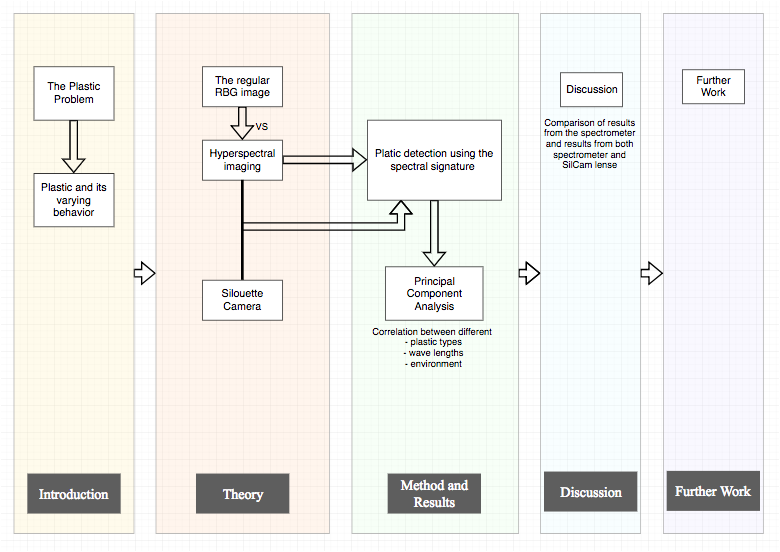
\includegraphics[width=\linewidth]{Images/outline.png}
  \caption{Thesis Outline, roughly sketched}
  \label{fig:outline}
\end{figure}

 % includes latex files from the same directory
\chapter{Today}
\label{chap:today}

\todo[inline, color=orange!40]{Tenker å utbroderer mer her - bruksområder og fly/AUV og ROV? Burde jeg også her ha med deler av seksjonen om plast fra motivation}

\begin{comment}
Marine biological diversity is already exposed to climate change, overfishing and other man-made disruptions. As if this were not enough, plastic pollution also causes huge damage to the marine environment. (*)
\\
335 million metric tons of plastic was produced in 2016. %(https://www.statista.com/statistics/282732/global-production-of-plastics-since-1950/)
It is projected that the production will nearly double within the next 10-15 years
%https://wedocs.unep.org/bitstream/handle/20.500.11822/25398/WED%20Messaging%20Two-Page%2027April.pdf?sequence=12&isAllowed=y
\\\\

Kanehiro et al. (1995) states that plastic accounted for 80-85 percent of the seabed waste in Tokyo Bay in the 90's. (*)
This is a striking finding, considering that most plastic residues are floating to some degree. Different types of plastic have different densities. Some types have higher density than water and float, while other types are denser than water. This contributes to the fact that plastic can be found throughout the sea column, and is present in many ecosystems. For instance, plastics have been found in the digestive system of organisms of all sizes, from small marine invertebrates to whales.
\\\\
Polyethylene bags, operating in the ocean currents, have a large resemblance to the predators targeted by turtles. (*) Plastic debris can thus prevent their survival (Bugoni et al., 2001, Duguy et al., 1998). The ingestion of plastic debris can, among other things, reduce food intake, cause internal damage, strangling (hvordan bøyes dette) or even death after blockage of the intestinal tract. (Zitko and Hanlon, 1991).
\\\\
Plastic is also a potential carrier of chemicals and can absorb bacteria already present in the ocean, including polychlorinated biphenyls (PCBs). (*) PCBs are harmful chemicals, even in very low amounts. The ingestion of PCB can cause reproductive disorders, change the hormone levels and increase the risk of several diseases. In some cases, an intake may lead to death [(Ryan et al., 1988, Lee et al., 2001)]. Ryan et al. (1988) proved that PCB in the bird's tissue originates from plastic particles. Plastic pellets can thus be transporter for PCB in marine food chains (Mato et al., 2001).
\\\\
Furthermore, different types of bacteria are attracted to free floating marine debris. These are better known as “hitch hikers”, and can threaten sensitive coastal environments, as the bacteria are far from their natural habitats. 
%(Environmental implications of plastic debris in marine settings-entanglement, ingestion, smothering, hangers-on, hitch-hiking and alien invasions Murray R. Gregory)
\\\\
Some phyto-plankton eating species are particularly exposed, as microplastic easily can be confused with phyto-plankton. One of the most common types of microplastics, polystyrene (PS), has shown to affect the ability to reproduce. %(http://www.pnas.org/content/113/9/2430).
%* = The pollution of the marine environment by plastic debris: a review Jose G.B. Derraik *
\end{comment}
%\section{Today}
\noindent
Solving today’s plastic problem is not an easy task - especially when plastic and microplastic are not only present in the water surface, but in the entire water column. Imagine multiplying the entire ocean surface with a few hundred meters dept. This leaves an almost impossible starting point. In addition, there are continuous currents and motion, allowing a large spread. On top of it all, the deep sea is difficult to reach, and if reaching it, poor sight is often a fact. So, what have been done so far in order to solve this plastic problem?
\\\\
The problem with plastic is becoming an increasingly known problem. Since plastic contamination and many of its consequences are visible to the naked eye, few people can deny that the pollution of plastic is a fact. Nevertheless, it is not enough to be aware of the problem – the world must cooperate and act. Today there are solutions like ocean cleanup, etc\todo{mer av dette}. The challenge with these solutions is that they do not necessarily go towards high concentrated areas. Today we know that large pieces of plastic travel to the garbage patch ....\todo{og dette} Nevertheless, the entire ocean needs to be mapped. %(Evidence that the Great Pacific Garbage Patch is rapidly accumulating plastic 2018, L. Lebreton1,2, B. Slat1, F. Ferrari1 – mer herfra). 
\\\\
One obvious requirement when mapping and cleaning the ocean of plastic, is the availability of an instrument able to detect plastic in the ocean separating it from the rest of the ocean particles. This is where the field of spectroscopy enters the court. The development of image detectors, especially the two-dimensional silicon charge coupled device (CCD), has revolutionized image spectroscopy. CDD provides information on the distribution of photon intensity along the spectrograph's entrance slit. The distribution of entrance slit into different wavelengths and intensities, has made it possible to reconstruct detailed images at high spatial (defined as 1 cm) and spectral (defines as 1 nm) resolution. This makes a hyperspectral imager particularly suitable, as it consists of a spectrometer equipped with this charge coupled device (CCD). 
% (Development of hyperspectral imaging as a bio-optical taxonomic tool for pigmented marine organisms - geir)
\\\\
%Use of Underwater Hyperspectral Imager (UHI) in Marine Archaeology 2014, Øyvind Ødegård1,3, Geir Johnsen2 and Asgeir J. Sørensen1
Hyperspectral imagery is defined as images that contain a spectrum of reflected light with a spectral resolution of 1-5 nm per image pixel. The object of interest, from now on denoted OOI, will absorb, scatter and reflect light of different portions of the visible spectrum. This will in sum give them their unique optical fingerprints, which can be used for classification with high degree of confidence.
\\\\
%(BASIC HYPER SPECTRAL IMAGING F. SIGERNES)
%G. Vane, ed., Imaging Spectroscopy II, Proc. SPIE 834, 1988.
%W.L. Wolfe, Introduction to Imaging Spectrometers, Vol. TT25 of Tutorial Text Series, SPIE Press, Bellingham, Wash., pp. 1-147, 1997.
The last decade, most of the work and discovery in hyperspectral imaging, have been within space and air-born sensors. Here, the instrument has proven to be a particularly powerful remote control tool. It is not until recently that the technology has been tested underwater. As the sea is not stagnant and objects in water can behave differently than in air, new challenges can occur. Nevertheless, research shows that the technology is promising, also underwater, and can be a very useful tool when detecting microorganisms.
\\\\
%In addition, work on detection and classification of plastic in the sea, has been conducted, using hyperspectral imaging underwater. \todo{mer fra bert sitt arbeid}
%Bert: http://journals.sagepub.com/doi/pdf/10.1255/jnirs.1212 (mer herfra). 

\section{Near Infrared Light}
%https://oceanoptics.com/plastic-recycling-nir-spectroscopy/  !!!

% https://www.researchgate.net/profile/Hamed_Masoumi/publication/285330830_Identification_and_classification_of_plastic_resins_using_near_infrared_reflectance_spectroscopy/links/572af79808aef7c7e2c5026d/Identification-and-classification-of-plastic-resins-using-near-infrared-reflectance-spectroscopy.pdf?origin=publication_detail 

Experiments analyzing the wave spectra of different types of plastics, have already been conducted. However, the results has been directed towards viewing the wave length interval describing near infrared light (NIR). Although the use of infrared light is an effective means when doing observation on land, light is rapidly attenuated by seawater which makes this approach far less effective when taking the problem below surface.
\\\\
Therefore, experiments using hyperspectral imaging in the spectra of visual light is on the agenda for this thesis. 
\\\\

\section{SilCam}
On a final note, the Silhouette camera (SilCam) developed by SINTEF, is also interesting in this matter. This technology is different, as it utilizes a light source behind the object to be identified to clearly see the outline of the target. Simplified, the hyperspectral imagery extracts the contents of what is depicted, while the SilCam captures the exterior. The question is, can these two methods compliment each other and give an even better way of detecting microorganisms? This has never been tried before..

%JEG ER VELDIG USIKKER PÅ OM DENNE BØR KOMME HER, SOM EN TEASER TIL NOE SOM EGENTLIG KOMMER I FURTHER WORK OG DERMED I NESTE RUNDE...
\chapter{Theory I - Optics}
\label{chap:theory1}
%- Hva karakterieserer plast utifra hva vi vet
%- ulike sensorer for deteksjon og kartlegging (vise sammenhengen til dette og en bredere oversikt - dette blir isåfall bare her, men tas ikke med videre - i metode kan vi heller si at vi avgrenser mot cam)
%- aktuelle sensorer 
%- sensorbærende plattform
%- PCA og singular value Decomp

The lecture notes from TTK20 [kilde] has been used in large part throughout this chapter. The following sections have this reference as their main reference: 3.1 Light, 3.2 Interference, 3.3 Diffraction, 3.4 The GRISM, 3.7 Properties of Photons and 3.9  System Optics. 

\section{Light} \label{sec:light}
%Color Registration of Underwater Images for Underwater Sensing with Consideration of Light Attenuation
%https://ieeexplore.ieee.org/stamp/stamp.jsp?tp=&arnumber=4209801
Light is electromagnetic radiation. The human eye can detect electromagnetic radiation within wavelengths of 400 and 750 nm, approximately. This electromagnetic spectrum is called visible light. Radiation with shorter wavelength than 400 nm is called ultraviolet, whereas infrared radiation has longer wavelength than visible light.
\\\\
When light from a light source hits an object surface, the light is reflected before eventually reaching the eye. In this task, the endpoint will not only be the human eye, but other viewpoints, for instance a camera lens. The observation of the reflected colors in the viewpoint, is affected by properties of object surfaces, the light intensity of light source and traveling distance of the light.
\\\\
%PDF FRA TTK20
Breaking down the definition of light, light can be defined as tiny packets called photons. The properties addressed to the photons are wave like. Because of this, the wave of light can be represented as a sine wave. The wave amplitude in 2D can be expressed as follows: 

\begin{equation}
    E(x,t) = E_0 sin(kx+\omega t)
    \label{eq:aml2d}
\end{equation}
$E_0$ represents the maximum amplitude of the wave. The wave repeats itself periodically with the period T. k is the wave number defined by $k= \frac{2 \pi}{\lambda}$, while $\omega$ is the angular velocity expressed as $k= \frac{2 \pi}{T}$.
\\\\
The wave can also be expressed as the real part of a complex number, $z = E_0(cos(\phi) + i sin(\phi))$, when $\phi$ is the phase shift represented by $\phi = kx + \omega t$. Using Euler's formula: $e^{i \phi} = cos(\phi) + i sin(\phi)$, a 3D wave can be expressed by: 

\begin{equation}
    \textbf{E}(\textbf{r},t) = \textbf{E}_0 e^{i \phi},
    \label{eq:aml3d}
\end{equation}

where $\textbf{r}$ is the position of the phase now defined as 

\begin{equation}
    \phi = \textbf{k}\cdot \textbf{r} - \omega t + \xi,
    \label{eq:phase}
\end{equation}

where $\xi$ is the initial phase of the wave. 
\\\\
However, this equations above is representing no more than one wave. Two waves not interacting with each other will propagate like represented above, but what happens when two or more waves meets and in fact do interact with each other? 

\vspace{1.3cm}
\section{Interference}
Interference consider the case when two or more waves act together. Starting with two waves, respectively $S_1$ and $S_2$, interacting with each other at P as illustrated in Figure \ref{fig:interference}. Of equation \ref{eq:aml3d}, the $S_1$ and $S_2$ are represented by

\begin{equation}
    \begin{split}
    \textbf{E}_1 = \textbf{E}_{01} e^{i \phi_1}\\ %\text{\hspace{0.6cm}and\hspace{0.6cm}}
    \textbf{E}_2 = \textbf{E}_{02} e^{i \phi_2}
    \end{split}
    \label{eq:2int}
\end{equation}
\\\\
with their associated phase shift expressed as presented in equation \ref{eq:phase}:
\begin{equation}
    \begin{split}
    \phi_1 = \textbf{k}_1\cdot \textbf{r}_1 - \omega t + \xi_1\\
    \phi_2 = \textbf{k}_2\cdot \textbf{r}_2 - \omega t + \xi_2
    \end{split}
    \label{eq:2intphase}
\end{equation}
\begin{figure}[h]
  \centering
    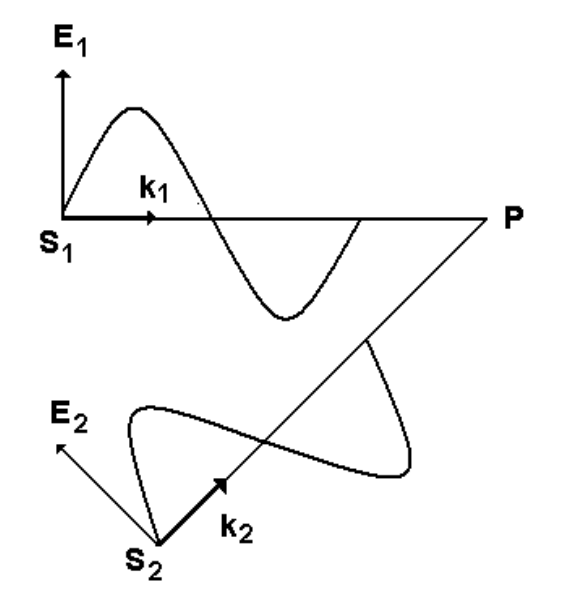
\includegraphics[width=0.3\textwidth]{Images/theory/interference.png}
    \caption{Two waves, $S_1$ and $S_2$, interfering}
    \label{fig:interference}
\end{figure}
Of Figure \ref{fig:interference}, one can conclude that the resulting wave, $\textbf{E}$ must be the sum of the two vectors interacting, $\textbf{E} = \textbf{E}_1 + \textbf{E}_2$. This applies to the resulting phase difference too, which thereby can be retrieved from equation \ref{eq:2intphase}: $\sigma = \textbf{k}_1\cdot \textbf{r}_1 - \textbf{k}_2\cdot \textbf{r}_2 + (\xi_1 - \xi_2)$. Now, the intensity of the final wave can be found by multiplying this resulting wave-vector, $\textbf{E}$, with its conjugate, $\textbf{E}^*$: 

\begin{equation}
    I = \textbf{E} \cdot \textbf{E}^* = \textbf{E}_{01}^2 + \textbf{E}_{02}^2 + 2\textbf{E}_{01}\cdot \textbf{E}_{02} cos(\sigma)
    \label{eq:two-wave-intensity}
\end{equation}
\\\\
The intensity in the equation above, eq \ref{eq:two-wave-intensity}, represents constructive interference at its maximum, whenever $cos(\sigma)$ is equal to 1, and expresses destructive interference at its minimum, when $cos(\sigma)$ equals -1. Constructive interference is hence present when the phase shift, $\sigma$ is expressed as:

\begin{equation}
    \sigma = 2 n \pi,
    \label{eq:maks}
\end{equation}

where n is the spectral order, a positive or negative integer. 
\\\\
Now, let us apply this to N number of waves, with several wave sources, up to $S_N$, as displayed in the figure below, Figure \ref{fig:Ninterference}.
\begin{figure}[h]
  \centering
    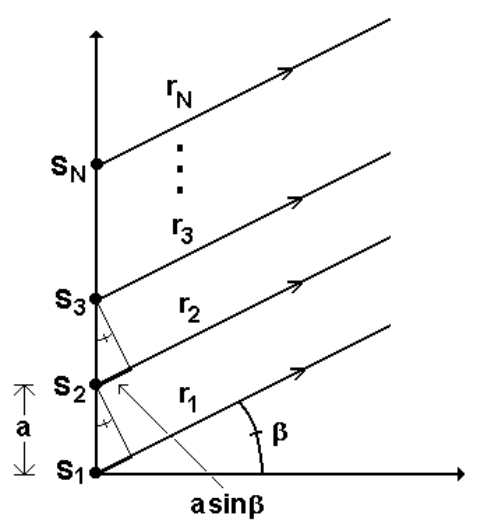
\includegraphics[width=0.3\textwidth]{Images/theory/Ninterference.png}
    \caption{N number waves propagating with a constant distance a}
    \label{fig:Ninterference}
\end{figure}
\\\\
The N waves are emitted by $S_N$ coherent and monochromatic sources separated by a distance, $a$. As the waves are coherent, the phase difference between the waves are constant. This means that the second term in equation \ref{eq:2intphase} can be ignored because $\xi_1$ = $\xi_2$ = ... = $\xi_N$. The phase difference is thus only due to the path difference between the waves, $\sigma = \textbf{k} \cdot \textbf{r}$. Of Figure \ref{fig:Ninterference}
$\textbf{r}$ can be retrieved as $a sin (\beta)$, while $k= \frac{2 \pi}{\lambda}$. Combining this with equation \ref{eq:maks}, $\textit{the grating equation}$ is found: 
\begin{equation}
    n \lambda = a sin(\beta)
    \label{eq:transgrating}
\end{equation}

\vspace{1.3cm}
\section{Diffraction}
While interference is a result of individual sources
interacting with each other, diffraction is present when a wave is distorted by an external object, with a comparable dimension to the wavelength of the wave. The figure below, Figure \ref{fig:diffraction} exemplifies diffraction with a port entrance wall as the external object. 
\begin{figure}[h]
    \centering
    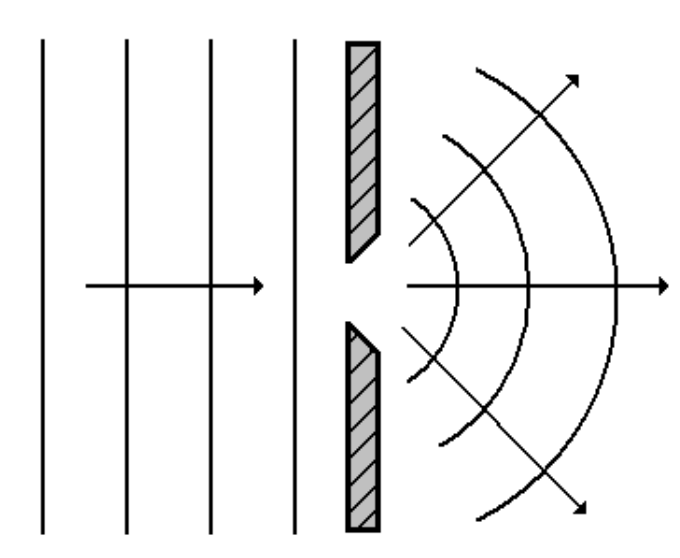
\includegraphics[width=0.3\textwidth]{Images/theory/diffraction.png}
    \caption{Diffraction as a result of waves hitting an entrance port}
    \label{fig:diffraction}
\end{figure}
\\\\
When the waves hit the external object in the figure above, a number of new waves originated from only one propagating wave, will be born. These children waves will, in turn, hit each other. This way, diffraction on the finite wave can be calculated as interference of the wave itself.

%TIL GRISM: 
%that the location of the intensity maxima for each order increases for increasing wavelength. This effect is the opposite of what happens with a prism, where there are no spectral orders and blue light is more refracted than red.

\subsection{Reflective Gratings}
The grating equation in \ref{eq:transgrating} assumes a grating transmitting light. The reflective grating, however, reflects the light. This grating can be thought of as a polished surface with parallel grooves - as shown in Figure \ref{fig:refgrating}. Between the grooves, parallel mirrors constitutes the grating, each mirror acting as a source of interference. 
\begin{figure}[h]
    \centering
    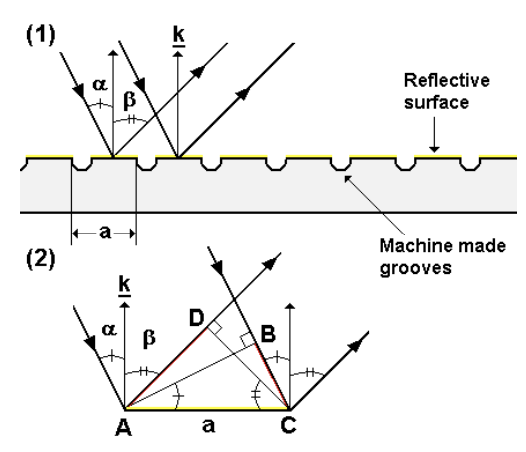
\includegraphics[width=0.4\textwidth]{Images/theory/refgrating.png}
    \caption{(1) Reflective
grating. (2) Resulting rays, where the red lines describe the associated phase difference}
    \label{fig:refgrating}
\end{figure}
\\\\
As explained in Section \ref{sec:light}, the phase difference of waves propagating from coherent sources is $\sigma = \frac{2 \pi}{\lambda} \cdot \textbf{r}$. Of the figure above, Figure \ref{fig:refgrating}, $\textbf{r}$ can be calculated as $(BC - (-AD))$. Based on this, the phase difference as a function of reflective grating can be presented as:
\begin{equation}
    \sigma = \frac{2 \pi}{\lambda}(BC + AD) = \frac{2 \pi}{\lambda} (a sin(\alpha) + a sin(\beta))
\end{equation}
\\\\
At maximum intensity (equation \ref{eq:maks}), the reflecting grating equation is found:
\begin{equation}
    n \lambda = a (sin(\beta) + cos(\alpha))
    \label{eq:refgrating}
\end{equation}
\\\\
Once again, n is the spectral order. $\alpha$ is the incident angle, and $\beta$ represents the diffracted angle of the grating.
\\\\
\subsection{Angular Dispersion}
Angular dispersion is a measure of how the diffracting waves are spread, per unit wavelength. The angular dispersion of a grating is defined as $d\beta/d\lambda$. This can be derived by differentiating the grating equation, equation \ref{eq:refgrating}. 
\begin{equation}
    \frac{d\beta}{d\lambda} = \frac{n}{a cos(\beta)}
    \label{eq:angdisp}
\end{equation}
\\\\
\section{The GRISM} \label{sec:grism}
A GRISM is a combination of a grating and a prism - hence the name. The GRISM is a prism stacked in series with a transmission grating, as can be observed in Figure \ref{fig:grism} below.
\begin{figure}[H]
    \centering
    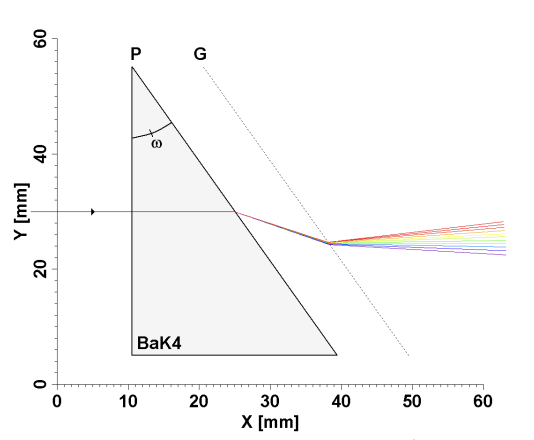
\includegraphics[width=0.5\textwidth]{Images/theory/GRISM.png}
    \caption{Light passing through a prism, P, dispersing blue light more than red, and a grating, G, diffracting red light more than blue}
    \label{fig:grism}
\end{figure}
\\\\
\noindent
For a grating, the intensity maximum for each spectral order, n, increases with increasing wavelength. A prism however, have no spectral orders and refracts blue light more than red. The net effect is a compact spectrum able to obtain a straight through center wavelength, parallel to the optical axis of the system. This on-axis effect, makes it easy to stack additional optics in both ends - the front and the back side of the GRISM. Due to absence of off-axis effects, image quality is preserved.
\\\\
When calculating the angular dispersion of a GRISM, the result is equal to the angular dispersion of a grating (equation \ref{eq:angdisp}), except for one additional term. This turns out to be a non-negative term, implying that the GRISM has an increased angular dispersion compared to a grating alone.

\vspace{1.3cm}
\section{The Behavior of Light in Air}
Light in air behaves differently than in water. In air, the light will not be attenuated, which means that the reflection can be expressed by the light intensity, $I_ {\lambda}$ (eq \ref{eq:int}), describing the colors observed on the object.
\begin{equation} \label{eq:int}
    I_ {\lambda} (L, z) = \frac{S \cdot \kappa_{\lambda}\cdot cos^{3}\cdot (\alpha)}{z^2}
\end{equation}
\\\\
In equation \ref{eq:int}, $I_{\lambda}$ represents the light intensity at a given wavelength, lambda, while S is the light source. L is the distance between the object and the viewpoint, while z describes the distance from the object to the light source. Furthermore, $\kappa_{\lambda}$ describes the reflectance ratio of the object's surface at a given wavelength, $\lambda$. $\alpha$ is the angle between the ray vector from the light source and the normal vector of the object surface.
\begin{figure}[H]
\centering
  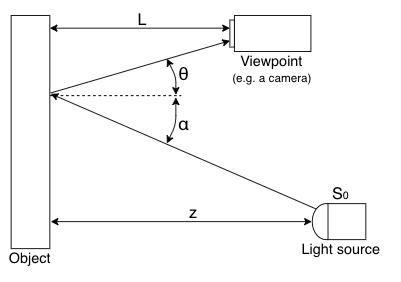
\includegraphics[width=8cm]{Images/theory/reflectance.png}
  \caption{Light refraction in liquid}
  \label{fig:reflectance}
\end{figure}
\\\\
\noindent
However, it is different if we do the same underwater. In water, light attenuation will be present and affect how the light is reflected. This will be elaborated in the following section.

\vspace{1.3cm}
\section{The Behavior of Light in Water}
%The light intensity decreases with the distance from objects in water by light attenuation depending on the wavelength of light. Red light decreases easier than blue light in water [E. O. Hulburt: “Optics of Distilled and Natural Water,” Journal of the Optical Society of America, Vol.35, pp.689–705, 1945].
The reason why the color of objects is different under water and in air, is that the light intensity, in water, decreases with the distance (r) to the object. This is, as mentioned, due to light attenuation, which again depends on the wavelength of the light. %([E. O. Hulburt: “Optics of Distilled and Natural Water,” Journal of the Optical Society of America, Vol.35, pp.689–705, 1945].) 
\\\\
From figure \ref{fig:lightinwater}, it can be observed that the intensity of the different colors decreases differently, even at the same distance, r. If the light source is 2 m away, red light will shine at half intensity, while blue light remains close to unchanged. At a distance of 20 meters, blue light will brighten at half-intensity. In this case, red and orange color will disappear.
%Color Registration of Underwater Images for Underwater Sensing with Consideration of Light Attenuation
%https://ieeexplore.ieee.org/stamp/stamp.jsp?tp=&arnumber=4209801
\begin{figure}[H]
\centering
  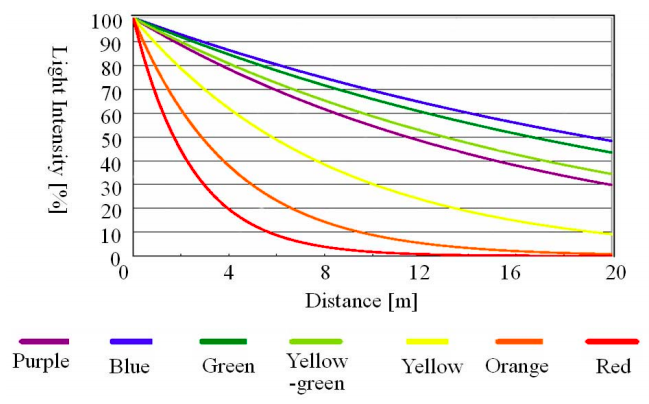
\includegraphics[width=9.5cm]{Images/theory/intensity.png}
  \caption{Light intensity in water.}
  \label{fig:lightinwater}
\end{figure}
\\\\
\noindent
As shown in the figure \ref{fig:lightinwater}, the light intensity decreases exponentially. The figure, is based on the following equation for the light source, S. 

\begin{equation} \label{eq:source}
S_{\lambda} (z) = S_0 \cdot exp (-c_{\lambda} \cdot r)
\end{equation}
\\\\
In eq \ref{eq:source}, $S_{\lambda}$ describes the light intensity at wavelength $\lambda$, while $S_0$ is the intensity at the light source. Furthermore, r describes the distance between the light source and the viewpoint, while $c_{\lambda}$ is the attenuation coefficient of the wavelength $\lambda$, illustrated by figure \ref{fig:attcoeff}.
\\\\
By taking the attenuation coefficient, $c_{\lambda}$, into consideration, the light intensity in water can be expressed by the following similarity. 

\begin{equation} \label{eq:intw}
    I_ {\lambda} (L, z) = \frac{S \cdot \kappa_{\lambda}\cdot cos^{3}\cdot (\alpha)}{z^2} \cdot exp \left(-c_{\lambda}\left(\frac{z}{cos(\alpha)}\frac{L}{cos(\theta)}\right)\right)
\end{equation}
\\\\
Interpreting eq \ref{eq:intw}, the intensity of light decreases when $c_{\lambda}$ increases. If $c_{\lambda} = 0$, meaning the light attenuation not being present, the resulting intensity becomes the same as the light intensity in air, eq \ref{eq:int}. 

\begin{figure}[H]
\centering
  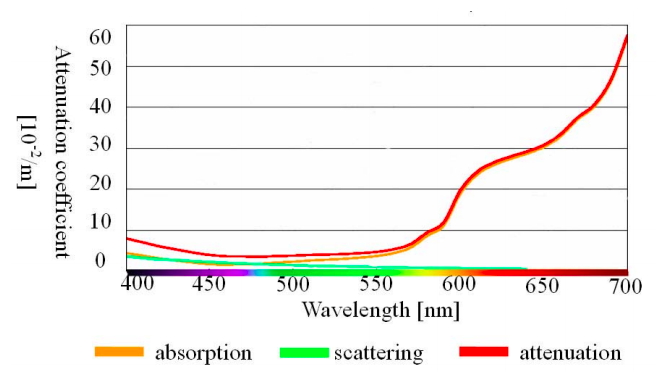
\includegraphics[width=9.5cm]{Images/theory/attcoeff.png}
  \caption{Attenuation coefficient}
  \label{fig:attcoeff}
\end{figure}


%Attenuation coefficient consists of absorption coefficient and scattering coefficient, because light attenuation consists of light absorption and light scattering. Attenuation coefficient of water changes very much with the wavelength of light. Consequently, observed colors changes in underwater environments.


%Stereo Measurement of Objects in Liquid and Estimation of Refractive Index of Liquid by Using Images of Water Surface
%http://www.robot.t.u-tokyo.ac.jp/~yamashita/paper/B/B047Final.pdf
\noindent
Note: If cameras and objects are in the different condition where the refraction index differs from each other, several problems occur and a precise measurement cannot be achieved.

\subsection{Near Infrared Light Transmission in Water} \label{sec:waterabs}
%http://www1.lsbu.ac.uk/water/water_vibrational_spectrum.html
Water absorbs wavelengths covering a wide range of electromagnetic radiation. For light with wavelengths larger than 200 nm, this absorption is due to rotational transitions and intermolecular vibrations. As the H2O-molecule has a particularly small moment of inertia on rotation, a rich vibrational-rotational spectrum appears, sometimes containing millions of absorption lines. 
\\\\
The water absorption spectrum is therefore very complex. The water molecule may vibrate in several ways, at several states affected by the environment. For the specific case of H2O, the absorption spectrum is displayed in Figure \ref{fig:absspec} below. The spectrum may vary based on the condition of the water and placement of measurement - for instance whether one looks at the open sea or the coastal areas. However, the trends represented in the figure, should more or less remain. The spectrum clearly shows how the water absorption is at its lowest in visible light, making this range of wavelengths more optimal when detecting objects underwater. Near infrared light on the other hand will quickly disappear over short distances. This could result in large variations in the resulting spectral signatures, leaving a possibly non-representable set of data.

\begin{figure}[H]
    \centering
    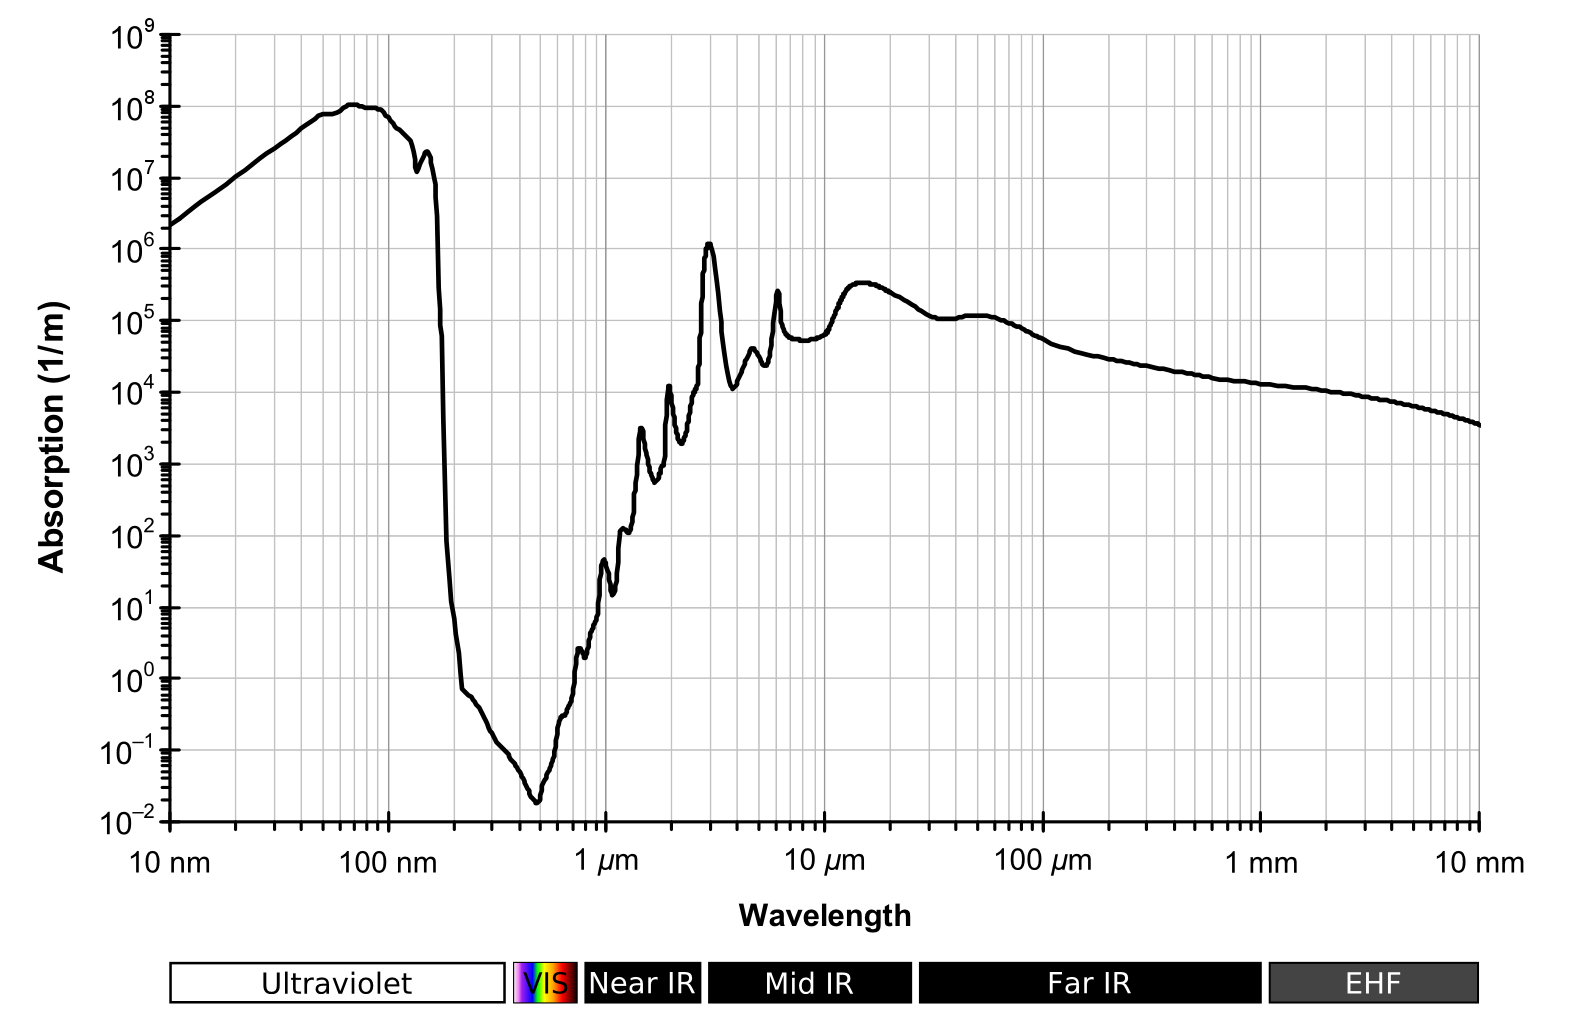
\includegraphics[width=8cm]{Images/theory/Absorption_spectrum_of_liquid_water.png}
    \caption{Absorption spectrum of liquid water}
    \label{fig:absspec}
\end{figure}


\begin{comment}
%PAPER: Identification and Classification of Plastic Resins using Near Infrared Reflectance PSpectroscopy: https://www.researchgate.net/publication/285330830_Identification_and_classification_of_plastic_resins_using_near_infrared_reflectance_spectroscopy

%https://oceanoptics.com/plastic-recycling-nir-spectroscopy/ Plastic Recycling with NIR Spectroscopy - denne inneholder signaturene til plast i NIR
%Another important observation in these experiments, is the condition of the microplastic used. The material is pure and white, making the results independent of color. 


Water absorption: 
%https://commons.wikimedia.org/wiki/File:Absorption_spectrum_of_liquid_water.png
This logarithmic (log-log) graph shows water’s absorption behavior at different colors wavelength. As seen in the graph, water absorption is minimised between 400 -600 nm


Light Transmission in the Ocean: http://www.waterencyclopedia.com/La-Mi/Light-Transmission-in-the-Ocean.html
https://manoa.hawaii.edu/exploringourfluidearth/physical/ocean-depths/light-ocean
\end{comment}



\vspace{1.3cm}
\section{Properties of Photons}
Photons...
\subsection{Flux}
\subsection{Intensity}
\subsection{Throughput}
\subsection{Etendue}



\vspace{1.3cm}
\section{Inherent Optical Properties}
%http://iopscience.iop.org/article/10.1088/0034-4885/36/12/002/pdf
%noe av dette har blitt sagt i hyp også:
When retrieving an optical fingerprint it is important to know the optical properties impacting the resulting signature. There are mainly three physical processes reducing the energy of light on its way to reaching the receiver. The OOI (the materials or the compositions of materials) will absorb, scatter and reflect light of different portions of the visible spectrum. This way, the material of the OOI and the wavelength will affect the properties of these processes. 
\\\\
Scattering, absorption and reflection are all results of photons interacting with the OOI. 
%http://www.oceanopticsbook.info/view/overview_of_optical_oceanography/inherent_optical_properties
\subsection{Absorption} \label{sec:abs}
During the photon-IOO interaction, the energy of the photon can be converted to another form, leaving the photon to disappear and hence the light to be absorbed. 
\\\\
%https://www.physicsclassroom.com/class/light/Lesson-2/Light-Absorption,-Reflection,-and-Transmission
Atoms and thereby molecules contain elections. Given the specific atom, these electrons hold a specific natural frequency. Whenever light hits these molecules, the electrons in that molecule will be given a vibrating motion if the frequency of the light is equal to the electrons natural frequency. This vibration is causing energy – energy taken from the lights photons. This way, the electrons absorb the energy of the light by turning it in to vibration energy, which cannot be converted back to light. 
\\\\
Different atoms will absorb light at different wavelengths, because they hold different sets of natural vibration frequencies. 

%{pluss coeff og internsitets-likn?}
%{pluss figur?}

\subsection{Scattering}
During the photon-IOO interaction, the photon might either change its direction, its energy or both. Either of these processes are called scattering. %http://iopscience.iop.org/article/10.1088/0034-4885/36/12/002/pdf 
More precisely, scattering can be defined as \textit{the change in direction of light flux produced by individual parcels of particulate matter called ‘scatterers’}. This means that light, or other moving particles, are forced to deviate from the straight trajectory they were on to being with, due to the collision between the light wave and the OOI. 
\\\\
%http://www.oceanopticsbook.info/view/overview_of_optical_oceanography/inherent_optical_properties 
As mentioned, these inherent optical properties are again dependent on many other properties. Different materials absorb and scatter very much differently as a function of wavelength. If comparing to particles with the same volume, they will scatter light differently if are of different shapes. Similarly, particles with exact same shape will scatter light differently whenever the volume of the particles differ. A change in the material, size or shape (or the composition of them) will give different IOPs. 
\\\\
In the ocean, the physical characteristics of the IOO are highly affected by the surroundings, implying that the IOPs are too. As an example, a change in the concentration of plankton or being in coastal waters instead of the open ocean, will contribute to a significant change in both the resulting absorption and scattering. 


\subsection{Spectral Reflectance}\label{sec:specref}
Light reflection from an object means that waves of light hitting the surface of the object is sent back from the surface. Reflection happens when the wavelength of the light waves do not match the natural vibration frequencies of the hit object. Whenever such waves of light strike the object, the electrons in the atoms of the object will vibrate. However, this is not the same type of vibration as the one discussed above (Section \ref{sec:abs}). Now, the electrons vibrate in small amplitudes for no more than brief periods of time. This causes the energy to re-emit as a wave of light, rather than turn into vibration energy an be absorbed at resonance vibration. 
\\\\
\begin{comment}
%Underwater hyperspectral imaging: a new tool for marine archaeology 2018, ØYVIND ØDEGÅRD,1,2,* AKSEL ALSTAD MOGSTAD,3 GEIR JOHNSEN,3 ASGEIR J. SØRENSEN, AND MARTIN LUDVIGSEN1
Raw data consists of more than upwelling radiance reflected from the object. Reflections from the water column, ambient light and noise sensors are all parts of the data collected. However, the spectral reflectance reference is independent of the illumination and the water column properties. 
\end{comment}
%Underwater hyperspectral imagery to create biogeochemical maps of seafloor properties 2013, G. JOHNSEN, NTNU
The spectral reflectance, also called the optical fingerprint can be described as a percentage of the light amount reflected off an object at each wavelength. As mentioned, different objects absorb and reflect different wavelengths. In plants, red and blue wavelengths are highly absorbed, leaving the reflected color to be more or less green. Mathematically speaking, the spectral reflectance, $R(\lambda)$ is upwelling irradiance coming off the object, $Lu(\lambda)$, divided by the spectral downwelling irradiance towards the object, $Ed(\lambda)$.
\\\\
%The use of underwater hyperspectral imaging deployed on remotely operated vehicles – methods and applications - geir og asgeir
\begin{equation} \label{eq:specref}
    R(\lambda) = \frac{Lu(\lambda)}{Ed(\lambda)}
\end{equation}
\\\\
Where $Lu(\lambda)$ denotes the raw data of the object, including signature from light source, while $Ed(\lambda)$ is the spectral radiance from measurements of spectrally neutral reflectance standard.
\\\\
Note: For eq \ref{eq:specref} to hold true, all surfaces are assumed to behave like Lambertian reflectors, meaning that the reference surface has a perfectly diffuse/matte property. This ensures that the radiant intensity, regardless of the reflected direction, is proportional to the cosine of the angle of the surface's normal. This is known as Lamberts Cosine law. 
%det siste er tatt fra TTK20-heftet


%The use of underwater hyperspectral imaging deployed on remotely operated vehicles – methods and applications - geir og asgeir

\vspace{1.3cm}
\section{System Optics} \label{sec:sysopt}
Rays travelling through a spectrometer can be described by an optical diagram like the one presented below in Figure \ref{fig:sysopt}.
\begin{figure}[H]
    \centering
    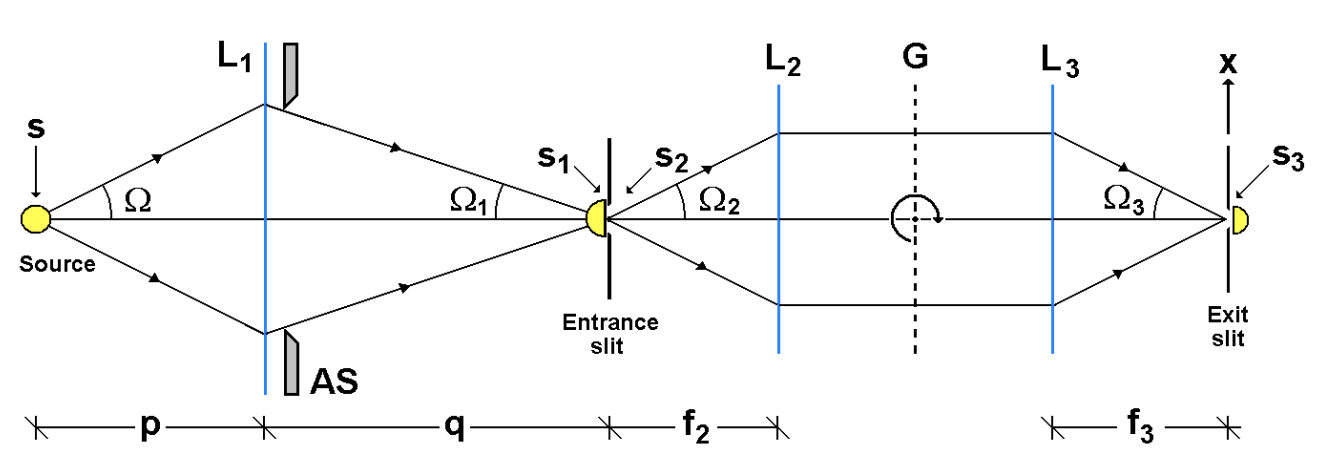
\includegraphics[width = 12cm]{Images/theory/sysop.png}
    \caption{Optical diagram of a Spectrometer}
    \label{fig:sysopt}
\end{figure}
\noindent
From the figure, one can extract $S$ as the source of light. $S$ illuminates the front lens, $L_1$, with the angle $\Omega$. Furthermore the front lens focuses the light onto the entrance slit, resulting in the imaged area, $S_1$. $G$ is the grating, either transmitting or reflecting, in which $L_2$ collimates with light passing through the entrance slit area, $S_2$, at an angle  $\Omega_2$. The diffracted beam of light from the grating is then focused onto the exit slit by $L_3$, as a function of wavelength. This makes $S_3$ the area of the diffracted entrance slit image. 
\\\\
$f_2$ and $f_3$ are the corresponding focal lengths of $L_2$ and $L_3$. Note that as long as $L_1$, $L_2$ and $L_3$ are able to focus or collimate the beam of light, they can be mirrors instead of lenses. 

%\subsection{Bandpass and Resolution}
\subsection{The GRISM Spectrograph}
In section \ref{sec:grism}, the GRISM, and how it could obtain a straight through center wavelength parallel to the optical axis, was elaborated. Therefore, using a GRISM as the dispersive element is popular when designing a spectrometer. Figure \ref{fig:grismspec} shows a typical 3D configuration of a GRISM spectrograph in hyperspectral image mode, illustrating the basic elements of hyperspectral imaging. Of the illustration, one can observe how the elements are stacked at the right next to each other (on axis), supporting the previous stated properties of the GRISM. This on-axis design reduces geometrical aberrations and thereby improves the resolution. 
\\\\
Similar to the spectrometer already discussed above (section \ref{sec:sysopt}), the front lens focuses light onto the entrance slit $S_1$, while $L_2$ collimates the GRISM. The diffracted light is then focused into the image detector (CCD), by $L_3$. 

\begin{figure}[H]
    \centering
    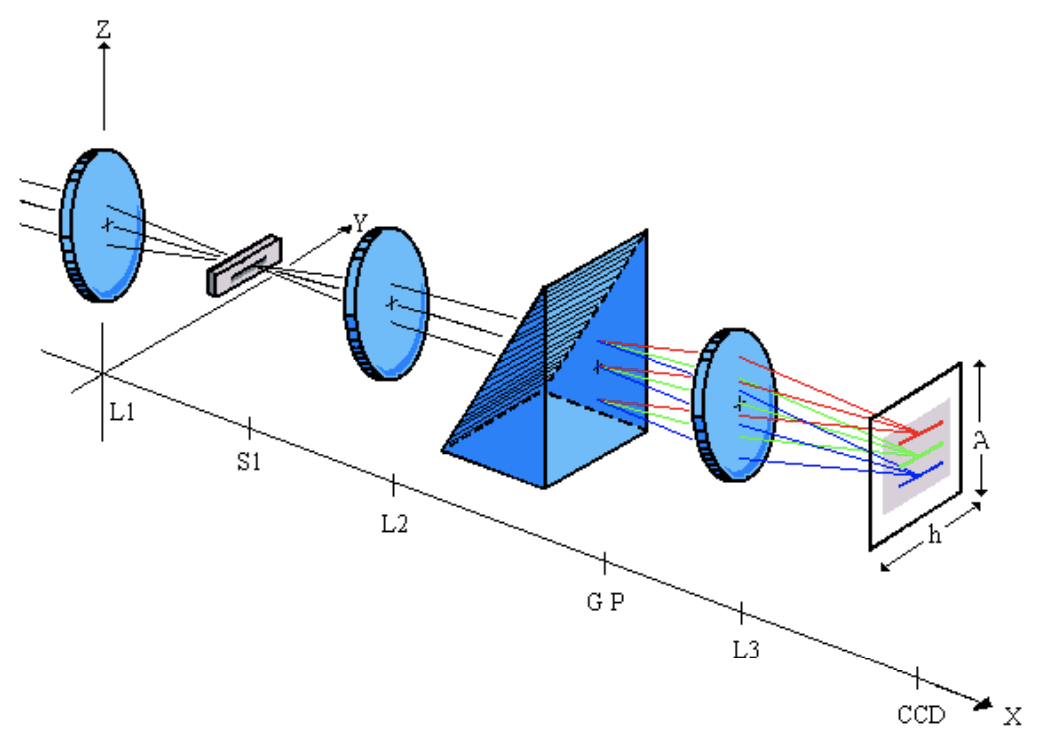
\includegraphics[width = 12cm]{Images/theory/grismspec.png}
    \caption{The GRISM spectrograph}
    \label{fig:grismspec}
\end{figure}


\chapter{Theory II - Imaging}
\label{chap:theory2}
\todo[inline, color = orange!40]{Imaging Precess}
%Denne skal jeg få tilsendt av Asgeir


\section{The Digital Image}
%evt Fysikken bak bildet 
%Info hentet fra bok: techniques and applications of hyperspectral image analysis
From the mid-20th century, images have been stored in digital format (Geladi and Grahn, 2000). A digital image is an array of rows (i) and columns (j) consistent of i x j gray-values. A gray-value, better known as an intensity or a pixel, is simply one of many small squares in an image. If the image is to consist of colors however, a third dimension is needed. This dimension is characterized as the depth, and can be found as the height in Figure \ref{fig:pogv}b). The depth is three layers deep, consisting of red, green and blue. What was previously a gray pixel is now a voxel illustrated in \ref{fig:pogv}b), with triplet of red, green and blue - each of which contains different information. Note that the height of the voxel is almost undetectable, as the voxel only consists of the tiniest distinguishable element of a 3D object.
\\\\
However, if the interval separating the layers is chosen to be a shorter wavelength, the number of layers will increase. The resulting image is then called a multivariate image, illustrated in Figure \ref{fig:pogv}c). If k denote the depth dimension and thus determine the number of wavelengths which in turn will constitute the number of layers, the resulting array will be of the size i x j x k.
\\\\
For the human eye to be able to perceive a color image, only three wavelengths/layers are needed, namely red, green and blue. It therefore rarely makes sense to create multiple layers unless the goal is to capture information the eye cannot see. This is where hyperspectral imaging enters the playing field, which by definition has more than 100 layers and can express each pixel as a spectrum.

\begin{figure}[H]
  \newcommand*\FigVSkip{0.5em}
  \newcommand*\FigHSkip{0.1em}
  \newsavebox\FigBox
  \centering
  % Top image is centered, so no need to get width
 \sbox{\FigBox}{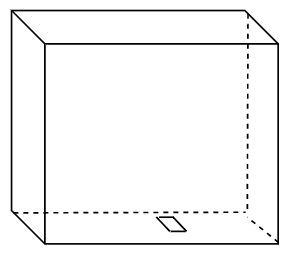
\includegraphics[scale=0.4]{Images/theory/pixel.png}}
  \begin{minipage}{\wd\FigBox}
    \centering\usebox{\FigBox}
    \subcaption{a) Pixel}
  \end{minipage}
    % Top image is centered, so no need to get width
 \sbox{\FigBox}{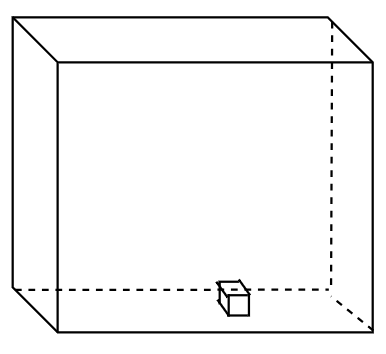
\includegraphics[scale=0.29]{Images/theory/voxel0.png}}
  \begin{minipage}{\wd\FigBox}
    \centering\usebox{\FigBox}
    \subcaption{b) Voxel}
  \end{minipage}
  % Save first image in a box to get the width
  \sbox{\FigBox}{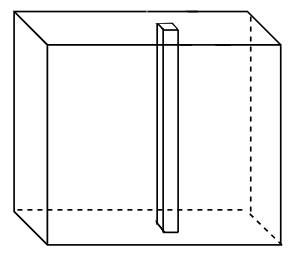
\includegraphics[scale=0.4]{Images/theory/voxel.png}}
  \begin{minipage}{\wd\FigBox}
    \centering\usebox{\FigBox}
    \subcaption{c) Multivariate Image}
  \end{minipage}\hspace*{\FigHSkip}
  % Save second image 
  \caption{Pixel, Voxel and Multivariate Image}
  \label{fig:pogv}
\end{figure}

\vspace{1.3cm}
\section{Hyperspectral Imaging}
%Info hentet fra yt
In order to study the reflecting light from the target, a spectrometer is needed. A spectrometer is an instrument that splits the incoming light into a spectrum. Measuring this reflectance spectra is the most common way to use hyperspectral imaging.
\\\\
Hyperspectral imaging uses a hyperspectral camera (imaging spectrometer) to collect spectral information. As mentioned, the difference between a hyperspectral image and a regular photo, is that the hyperspectral camera measures hundreds of thousands of spectra instead of single spectrum, creating not only a multispectral image, but a hyperspectral image. In contrast to multispectral imagers, which are sensitive in only a few selected wavebands, hyperspectral imagers (HI) measure the spectral reflectance per image pixel of the OOI, leaving a complete spectrum for each pixel in the image. %(Development of hyperspectral imaging as a bio-optical taxonomic tool for pigmented marine organisms - geir)
\subsection{On a Detailed Level}
%The Spatial Resolution
In detail, a spectrograph, illustrated in Figure \ref{fig:grismspec}, generates images from the entrance slit, as a function of wavelength (color). The amount of images detected by the CCD at the exit slit, is dependent on the entrance slit width and the element’s ability diffract the colors. The width of the exit slit being dependent on width of the entrance slit, among other things, can be seen from the equations in section.. describing optimal etendue \todo{legge inn dette I etendue osv}. A large amount of detected images at the exit slit will directly improve the spectral resolution of the instrument. The resulted image recorded by the CCD is called a spectrogram (an illustration of a spectrogram can be found as the last element in fig \ref{fig:grismspec}). The spectrogram contains both spectral and spatial information and can be described by the intensity distribution and position along the slit. 
\\\\
However, the information retrieved is information about the covered area of the target object, which is nothing but a very thin track covering only a small part of the object. In order to obtain the object's full spatial extent, the entire object surface needs to be sampled. 
\\\\
Now, how can this be done? The recording instrument must be moved relative to the target. The velocity, $\nu$ of the instrument is crucial, as the instrument will under sample (miss samples of the target area) if the distance moved during readout time, $\tau$, exceeds the length of the measured area, $dx$ (displayed in Figure \ref{fig:spatialres}). This requirement is shown in equation \ref{eq:req}.

\begin{equation}
    \nu \cdot \tau \leq dx
    \label{eq:req}
\end{equation}
This way, the image at the entrance plane moves across the slit so that the CCD can record spectrograms for each track of the object. This is called the push broom technique, which will be illustrated in Section \ref{sec:push}. When summarizing all samples, information on the continuous image can be retrieved.
\\\\
The required movement is based on the instrument and target moving relative to each other. Hence the movement can be created in two ways. Either the instrument can move, or the viewed target can be moved while keeping the imager still. If the target is located at a conveyor belt, it might be suitable to keep the instrument still. However, as mentioned, the magnitude of the relative movement is important. This means that if the conveyor belt is moving too fast, the instrument needs to move as well, in order to reduce the relative movement.
\\\\
Figure \ref{fig:spatialres} describes the situation where a hyperspectral imager is attached to an airplane moving at a velocity, $\nu$. In the illustration, $S$ is the slit, while $w$ is the associated width. $z$ describes the altitude above ground level. The front lens is denoted $L_1$, and has a focal length of $f_1$. 
\begin{figure}[H]
    \centering
    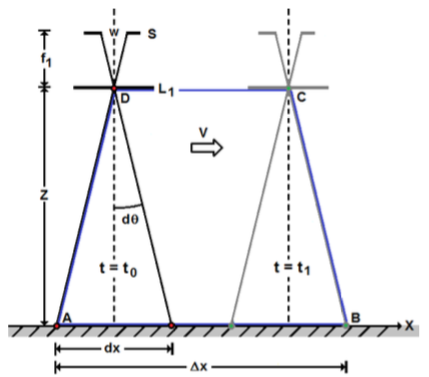
\includegraphics[height=7cm]{Images/theory/spatialres.png}
    \caption{Spatial resolution - Field of view (from a moving airplane)}
    \label{fig:spatialres}
\end{figure}
\noindent
It is common to believe that the spatial resolution is dependent on the number of pixels present along the wavelength axis of the detector. However, the amount of information is described by the number of spectral layers that hyperspectral imager can produce (illustrated as the height of the column in Figure \ref {fig:pogv}c)). The spectral layers define a dimension independent of the pixel-plane, only dependent on the bandpass (see section bandpass) and the spectral range of the instrument. Using similarity of form, $dx$ can be calculated from the lengths of the figure.
\begin{equation}
    dx = \frac{z \cdot w}{f_1}
    \label{eq:dx}
\end{equation}
Equation \ref{eq:dx} shows how $dx$ is connected to spectral bandpass through the slit width, $w$. 


\todo[inline, color=blue!30]{legg inn bandpass i teori del 1}
%Info hentet fra bok: techniques and applications of hyperspectral image analysis
 %oppsettene inkluderer lyskilde, et filtersystem som disperse the light into bands of wavelenghts, en sample. Hvis kilden inneholder et bredt lysspekter, kan man velge ut bølgelengder ved å bruke bandpass-filters etter ønske.


%The spectral information in every pixel creates a third dimension, providing a collection of data called a data cube. Now, how does this data differ from the data and images from other types of cameras? Digital camera, shoots the target in red, green and blue, in order to match the human vision. These camera leaves a combination of the three colors, which is what we can see with our eyes. This means that the information constituting the third dimension consists of nothing more than three colors, while the hyperspectral camera records hundreds of wavelengths. This way, the hyperspectral camera can collect more detailed information about the target, not only in visible light, but also in infrared and ultra violet. By combining different wavelengths, pixel by pixel, one can extract useful information about the properties of the target. 

\subsection{On an Environmental Level}
%Hyperspectral imaging and data analysis for detecting and determining plastic contamination in seawater filtrates, 2016,  Bert van Bavela
%http://journals.sagepub.com/doi/pdf/10.1255/jnirs.1212
\noindent
Concerning plastics, this translates to receiving information on both spatial location of plastic material, and the plastic materials composition. 
%Volent, Z., Johnsen, G., & Sigernes, F. (2007). Kelp forest mapping by use of airborne hyperspectral imager. Journal of Applied Remote Sensing, 1, 011503–011521.
%Volent, Z., Johnsen, G., & Sigernes, F. (2009). Microscopic hyperspectral imaging used as a bio-optical taxonomic tool for micro- and macroalgae. Applied Optics, 48, 4170–4176.
\\\\
%(Development of hyperspectral imaging as a bio-optical taxonomic tool for pigmented marine organisms - geir)
\noindent
HI and UHI can be used as a taxonomical identification tool to make optical fingerprints of marine organisms only if the pigment composition and corresponding absorption signature of the organism is known and can be used to verify the reflectance signature
\\\\
\noindent
When the hyperspectral camera is taken underwater, the lighting is limited. The UHI is therefore using its own light sources, in contrast to passive passive techniques using ambient light.
%(Development of hyperspectral imaging as a bio-optical taxonomic tool for pigmented marine organisms - geir) %The use of underwater hyperspectral imaging deployed on remotely operated vehicles – methods and applications - geir og asgeir
\\\\
\noindent
In this task, there are two methods for camera configurations, point scanning image and line scanning image.
\subsection{Point Scanning Image}
Point scanning image can be used to measure a complete spectrum in one spot/pixel. In every spot, all layers are measured vertically from this spot. To make the whole picture, the camera must scan across the entire surface, spot by spot.
\\\\
figuren er hentet fra boken, techniques and applications of hyperspectral image analysis, side 6

% \begin{figure}[H]
%   \includegraphics[height=12cm]{Images/theory/pointscan.png}
%   \caption{Set-up, Point Scanning Image}
%   \label{fig:pointscan}
% \end{figure}


\begin{figure}[H]
\centering
  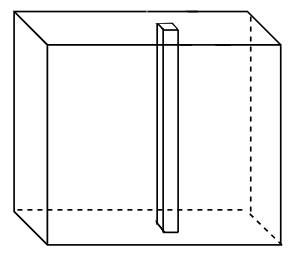
\includegraphics[height=6cm]{Images/theory/voxel.png}
  \caption{ Resulting scan}
  \label{fig:voxel2}
\end{figure}


\subsection{Line Scanning Image} \label{sec:push}
The line scanning image technique uses a two-dimensional detector, perpendicular/orthogonal to the surface of the measured target. This detector collects the spectrum of a whole line in the image, in one single scan. By moving the scan line with a push broom technique, one can map the entire image by combining all sets of spectra.
\\\\
figuren er hentet fra boken, techniques and applications of hyperspectral image analysis, side 7

% \begin{figure}[H]
% \centering
%   \includegraphics[height=12cm]{Images/theory/linescan.png}
%   \caption{Set-up, Line Scanning Image}
%   \label{fig:linescan}
% \end{figure}

\begin{figure}[H]
\centering
  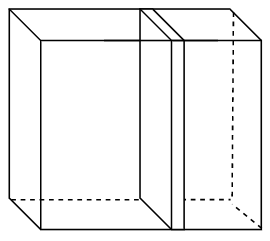
\includegraphics[height=6cm]{Images/theory/pushbroom.png}
  \caption{ Resulting scan}
  \label{fig:pushbroom}
\end{figure}

\vspace{1.3cm}
\section{SINTEF SilCam}
%https://github.com/emlynjdavies/PySilCam/wiki 
The silhouette camera, SINTEF SilCam, is a holographic imager designed to overcome the limitations in depth-of-field scenarios related to restricted path length, which is a challenge when using today's conventional lens-based imaging. The imager is developed by SINTEF with one of the experts, Emlyn Davies, in the front.
\\\\
In order to reduce noise, each image is corrected using a clean background. From this, it is possible to produce a logical image of the particles detected, containing only zeros and ones. In turn, particle properties for each particle can be calculated from the binary image.
\\\\
This way, the system can be used for both large- and small-scale experiments. In smaller scale, the SilCam is able to quantify the distribution of suspended material. Zoo-plankton, larger phyto-plankton, mineral grains and marine snow are all examples of objects the SilCam can detect. 

\chapter{Theory III - Data and Data Tracking} \label{cap:theory3}
This chapter presents ways of handling data. In this thesis, the data collected is regarding the five types of microplastic, also elaborated here. 

\section{Microplastic} \label{sec:microplastic}
%ha med hva def av mikroplast og de ulike plasttypene
%Kjemi
\todo[inline, color=orange!40]{ta med figur av alles struktur?}
\noindent
As mentioned, plastics have permeated almost every aspect of modern day life with its large applicability. We find plastics in the microchips in our computers, as well as in the bags we carry our groceries in. It seems that plastic covers a wide spectrum of applications.  One reason to this, is the many different types of plastic, covering different areas of need. Polyethylene (PE), polypropylene (PP), polyethylene terephthalate (PET), polyvinyl chloride (PVC) and polystyrene (PS), are the five most common types of plastic, in large part covering of the global plastic production. Besides containing Carbon-Hydrogen bindings, these are all structurally different and they are classified according to their chemical structure. In this section, these five types of plastic are presented in decreasing order. 
\\\\
%Plastic polymers commonly found in the environment are polypropylene (PP), polyethylene (PE), polyethylene terephthalate (PET), polystyrene (PS) and polyvinylchloride (PVC).8 Together these comprise 72.9 percent of the plastic produced globally.9

\subsection{Polyethylene}
The molecules in polyethylene (PE) has the chemical formula $C_2H_4$. Polyethylene is the most common type of plastic. The reason to its commonness is the broad application of it in consumer products. Plastic bags, bottles and food wrapping are good examples of polyethylene. However, these three products seem to have a significantly different material. For instance are plastic bags rarely as rigid and as bottles. This variation in polyethylene creates two sub-types defined by the degree of density – HDPE and LDPE, high-density polyethylene and low-density polyethylene respectively. 
\\\\
The LPDE-molecules are more branched, meaning that a chain is replacing for instance a hydrogen atom. As a result of this, the molecules are less tightly packed, leading to a lower density.  As LDPE has more branching than HDPE, its intermolecular forces are weaker. \todo{FIGUR av branch-forskjellene?}


\subsection{Polypropylene}
Polypropylene (PP) is the second most common plastic consistent of propylene with the chemical formula $C_3H_6$. PP has properties similar to polyethylene, but it is slightly harder and more resistant to fatigue. The plastic type is found in a variety of products like food packaging, labeling and clothing. 

\subsection{Polyvinyl Chloride}
%http://www.plasticmoulding.ca/polymers/pvc.htm
Polyvinyl chloride (PVC) with a number of vinyl chloride molecules formulated by $C_2H_3Cl$, is in third place of the most produced types of plastic. PVC can be both rigid and flexible. The rigid form is used in constructional application in piping and electrical wire insulation, while the softer and more flexible form is used in many applications replacing rubber. 

\subsection{Polyethylene terephthalate}
Polyethylene terephthalate (PET) consist of repeating ethylene terephthalate molecules, holding the chemical formula $C_{10}H_8O_4$. Typically PET is used in plastic bottles and in fibers for clothing. For the latter use, the type is commonly known as polyester. Depending on the specific particle's size and crystal structure, the semi crystalline material, PET, might appear transparent. 

\subsection{Polystyrene (PS)}
%https://www.azom.com/article.aspx?ArticleID=7915
Polystyrene (PS) is an inexpensive plastic type commonly used for packaging purposes, with the chemical formula being $(C_8H_8)_n$. PS increasingly exists in the outdoor environment, particularly along shores. The plastic is naturally clear, hard and brittle. The latter fact is perhaps the main reason to why larger pieces of PS easily turn into microplastic. 

\vspace{1.3cm}
\section{Georeferencing}
%http://www.gisresources.com/georeferencing-2/
In raster system, points are represented by single cells, lines by sequence of neighboring cells and area by collection of continuous cells
\\\\
%http://desktop.arcgis.com/en/arcmap/10.3/manage-data/raster-and-images/fundamentals-for-georeferencing-a-raster-dataset.htm
Georeferencing means to relate an internal coordinate system to a spatial coordinate system. The internal coordinate system could for instance be a raster image of a map. 
%http://www.gisresources.com/georeferencing-2/
Note that raster systems represents points by single cells and lines by several neighboring cells. Areas are represented by a collection of continuous cells. 
\\\\
In order to georeference an image, control points need to be established. These control points are identified as a series of known x- and y-coordinates, linking locations in the raster dataset to its correspondant location in the spatially referenced data. The desired objective is to assign these coordinate systems to each other with minimal residuals. This means that the distance between the control points’ actual coordinates and the coordinates predicted by the model is the smallest is can be, making the process as accurate as possible. This way, georeferencing can explain how data, such as GPS points, are related to images.

\vspace{1.3cm}
\section{Principal Component Analysis} \label{sec:pca}
This section contain knowledge gained in TTK19...
\\\\
The purpose of conducting a principal component analysis (PCA) is to extract the information from the data, while disregarding the noise, reducing the dimension of the dataset. The analysis converts a set of observations of possibly correlated variables into a set of values of linearly uncorrelated variables called principal components. These principal components will describe the overall variation of the dataset and thereby serve as a latent variable. 
\\\\
Now, how are these principal components found? Figure a) below describes the entire dataset with the dots describing single data observations. The analysis starts by finding the projection of each observation onto a line. The line is drawn with the purpose of explaining as many observations as possible with a minimal residual error, b). The distance from the origin to this projected point along the line is the score associated with the related observation. The direction of the line is now characterized with giving the largest variance of the scores, and is described by direction vectors called loadings. 
\\\\
%Simply put, the original data is estimated by multiplying the scores with the associated loadings.
This first line created is called the first principal component. The second principal component, c), is perpendicular to the first component’s direction and is otherwise found the same way. This way, the first principal component has the largest possible variance. Each following component will, in turn, have the highest variance possible under the constraint that it is perpendicular to the previous components. 

%FIGURENE:
%https://learnche.org/pid/latent-variable-modelling/principal-component-analysis/geometric-explanation-of-pca
\begin{figure}[H]
  \newcommand*\FigVSkip{0.5em}
  \newcommand*\FigHSkip{0.1em}
  \newsavebox\FigBox
  \centering
  % Top image is centered, so no need to get width
\sbox{\FigBox}{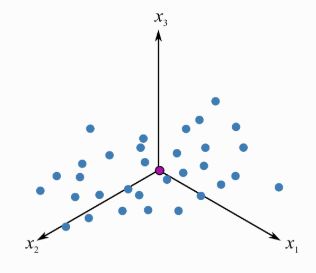
\includegraphics[scale=0.4]{Images/theory/koord.png}}
  \begin{minipage}{\wd\FigBox}
    \centering\usebox{\FigBox}
    \subcaption{a) Scaled and centered data observations}
  \end{minipage}
 \sbox{\FigBox}{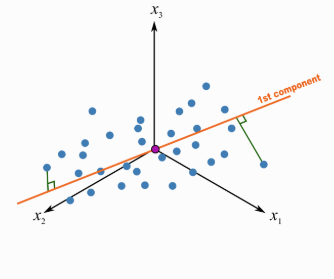
\includegraphics[scale=0.4]{Images/theory/1pc.png}}
  \begin{minipage}{\wd\FigBox}
    \centering\usebox{\FigBox}
    \subcaption{\newline b) Including first principal component}
  \end{minipage}
  % Save first image in a box to get the width
  \sbox{\FigBox}{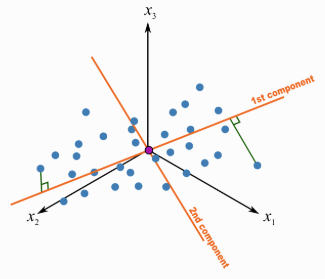
\includegraphics[scale=0.4]{Images/theory/2pc.png}}
  \begin{minipage}{\wd\FigBox}
    \centering\usebox{\FigBox}
    \subcaption{c) Including second principal component}
  \end{minipage}\hspace*{\FigHSkip}
  % Save second image 
  \label{head}
\end{figure}

\subsection{Scores, Loadings, F-residuals, Hotellings T^2 }
https://learnche.org/pid/latent-variable-modelling/principal-component-analysis/interpreting-the-residuals

\vspace{1.3cm}
\section{Sensor Carrying Platform}
%ulike sensorer for deteksjon og kartlegging (vise sammenhengen til dette og en bredere oversikt - dette blir isåfall bare her, men tas ikke med videre - i metode kan vi heller si at vi avgrenser mot cam. + aktuelle sensorer

 % could be called Methodology or methods or any filename  % could be results% could be results
\chapter{Method for Experimental Work}
\label{chap:method}
%In this chapter the methodology for the creation of the two models will be described.
This chapter defines the methodology and approach of the experimental work conducted at Trondheim Biological Station. Aksel Alstad Mogstad, one of the experts, supervised the entire experiment with steady guidance. The approach describing the processing and analyses of the data, done at a later stage, is presented towards the end of the chapter.

\section{Laboratory Testing}

\subsection{The Set-Up}
Figure \ref{fig:lab-set-up} contain images of the components used in the laboratory experiment. The spectrometer (a) was turned on and connected to the software OceanView 1.6.7 via a standard external computer. In OceanView, the spectrometer was sat to a constant temperature of 15 degrees (Celsius). The QR400-7-VIS-BX reflection probe (b) was connected to the spectrometer through one cable, and a light source through another. The cables are fiber optic, and are assumed to not have a noteworthy effect the results. The light source used was Schott KL1500 electronic light source (c), a 150 W halogen light delivering a constant spectral signature - after given some time to heat up. In addition, the reflection probe was placed in a reflective probe holder (d), angling the light output (and the sensor inlet) in order to avoid specular reflection. This angle was sat to 45 degrees and the distance to 1 centimeter.
\\\\
Furthermore, the reflective probe was placed over the object to be measured (d). Initially, this was the WS-1 Reflectance Standards (e) with 100 percent reflectance within the range of 250-1500 nanometers. This was measured in OceanView and sat the standard for white. The reflectance was assumed to be 100\% for the reflectance standard. Note that this is the Lambertian surface mentioned in Section \ref{sec:specref}. The reflectance standard calibrate the software such that all further measurement will be a relative size compared to the original standard white. An effect of measurements being relative to the original white is the accounting of, and subsequent omittance of the noise due to the light source. 



\begin{figure}[H]
  \newcommand*\FigVSkip{0.5em}
  \newcommand*\FigHSkip{0.1em}
  \newsavebox\FigBox
  \centering
  % Top image is centered, so no need to get width
 \sbox{\FigBox}{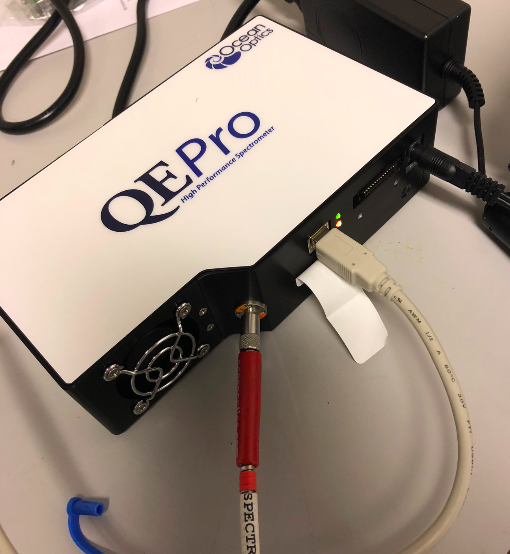
\includegraphics[height=5cm]{Images/method/qe-pro.png}}
  \begin{minipage}{\wd\FigBox}
    \centering\usebox{\FigBox}
    \subcaption{a) QE Pro}
  \end{minipage}
    % Top image is centered, so no need to get width
 \sbox{\FigBox}{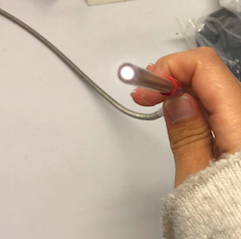
\includegraphics[height=5cm]{Images/method/light.png}}
  \begin{minipage}{\wd\FigBox}
    \centering\usebox{\FigBox}
    \subcaption{b) Reflection probe}
  \end{minipage}
  % Save first image in a box to get the width
  \sbox{\FigBox}{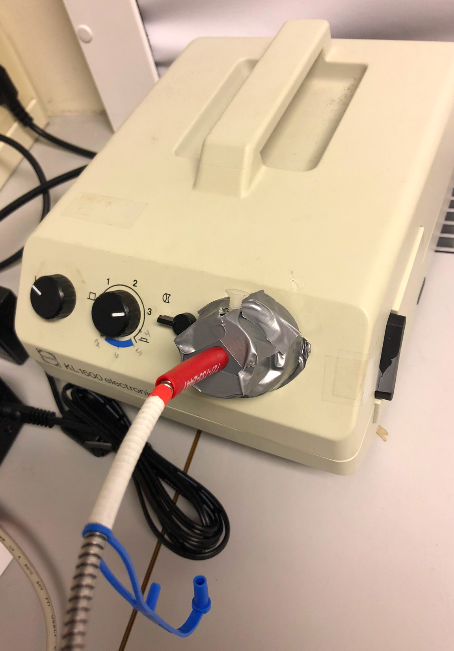
\includegraphics[height=5cm]{Images/method/lightsource.png}}
  \begin{minipage}{\wd\FigBox}
    \centering\usebox{\FigBox}
    \subcaption{c) Light source, Schott KL1500, 150 W halogen}
  \end{minipage}\hspace*{\FigHSkip}
  % Save second image 
\end{figure}

\begin{figure}[H]
  \newcommand*\FigVSkip{0.5em}
  \newcommand*\FigHSkip{0.1em}
  \newsavebox\FigBox
  \centering
  % Top image is centered, so no need to get width
 \sbox{\FigBox}{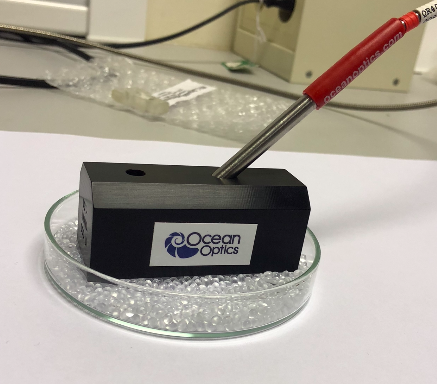
\includegraphics[height=4cm]{Images/method/setup.png}}
  \begin{minipage}{\wd\FigBox}
    \centering\usebox{\FigBox}
    \subcaption{d) Reflection probe holder from Ocean Optics}
  \end{minipage}
    % Top image is centered, so no need to get width
 \sbox{\FigBox}{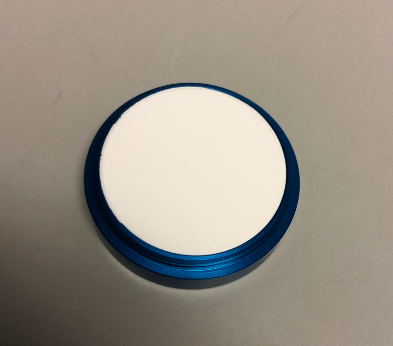
\includegraphics[height=4cm]{Images/method/lamber.png}}
  \begin{minipage}{\wd\FigBox}
    \centering\usebox{\FigBox}
    \subcaption{e) WS-1 Reflectance standard, lambertian surface from Ocean Optics}
  \end{minipage}
  % Save first image in a box to get the width
  \sbox{\FigBox}{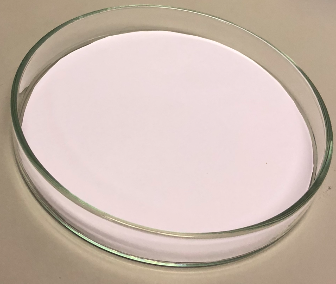
\includegraphics[height=4cm]{Images/appendix/papir.png}}
  \begin{minipage}{\wd\FigBox}
    \centering\usebox{\FigBox}
    \subcaption{f) Paper background}
  \end{minipage}\hspace*{\FigHSkip}
  % Save second image 
  \caption[The Laboratory Set-up]{The laboratory set-up}
  \label{fig:lab-set-up}
\end{figure}


\\\\
\noindent
In order to avoid further noise, the lab was kept as dark as possible to avoid ambient light. Light blocking blinds were used and to avoid the glare from the computer screen to affect the signature, the computer was covered behind a screen made of cardboard. Once the room was sufficiently dark, the spectrometer was turned on separately from the light source. This was done to measure the signal delivered from the sensor in completely dark environments. This dark noise could then be compensated for by the software. Throughout the experiment, the dark noise was only measured once - at the beginning of the experiment.
\\\\
Even though the reflectance standard is supposed to be 100\% reflective, there is still a possibility of achieving higher than 100\% which occurs in mirrors. The results would be saturation, which causes the measurement to flatten. As a consequence, one would lose information. As the plastic could contain mirror like properties, a margin was set in order to avoid saturation.
\\\\
Oceanview continuously sampled from the camera at a rate equivalent to the shutter speed - every 800 milliseconds. However, in order to obtain minimum amount of noise, the signature was more rarely updated. The software averaged the values obtained between each update. As a result, the obtained signature was an average of 5 scans. Therefore, the signature was updated every 4 seconds. As there should be no variation in the signature when measuring the same sample, the variation may be regarded as noise. 
\\\\
In addition, the delay in the system is irrelevant at this stage. This is due to the absence of a control system or other systems relying on delivering a real-time response to the signature.
\\\\
Going further, a layer of plastic was placed in a glass petridish with a double layer of white paper in the bottom. The layer of plastic was intended to be a single layer in order to see the effect of thickness on the see-through plastic. The petridish was used to contain the plastic, while the white paper was used to avoid the results of the see-through plastic to be affected by the background. The reflective probe holder was then placed over the specific plastic type to be measured. Each type of plastic was measured 10 times - each time a different place. The plastic types with variation in color was measured 10 times per color. This way, the different colored samples were possible to separate. The reflectance from the plastic pieces was then visualized in OceanView and ready for comparison. This process was iterated with different types of plastic. 
\\\\
The movement of the reflective probe holder can affect the scanner and thereby change the angle affecting the reflectance. In between samples and after conducting five samples of the same material, the the software was therefore calibrated with the standard white. Given the software’s relative measuring, this hopefully ensured the maintenance of correct reflectance for all signatures.

\subsection{Choice of Spectrum}
As discussed in Section \ref{lightinwater}, infrared and near-infrared light has a poor "performance" in water. Due to infrared and near-infrared light being low-energy it quickly disappears over a short distance in water. This will make it difficult to measure and could possibly result in large variations in the signature, which would be difficult to account for. This, in addition to information extracted from the water absorption figure, Figure \ref{fig:absspec} displayed in Section \ref{lightinwater}, point towards the visible light spectrum as the better alternative, underwater.
\\\\
Furthermore, higher wave lengths depicted high levels of noise and inconsistencies in the measured values. This was most likely due to the relative measurements of the software. The measured values are relative in the sense that the \textit{actual} measured value is divided by the reflective standard. The reflective standard yielded low values in the IR and NIR spectra. Since small values in the divisor cause large variations as it will be greatly multiplied, the variations were large. Also, UV-lighting and other light with wavelengths outside the visible spectrum were neglected.
\\\\
Because of all of the above, the visible spectrum was measured in the interval 400nm - 700nm. The resulting intensity was measured approximately every 0,758 nanometers. 

\section{Materials} \label{sec:material}
In order to cover a wide range of plastic, eventually turning into microplastic, the material tested were the most common types of plastic. Table \ref{tab:tested:plastic} shows the types of plastic tested, their state and additives:

\begin{center}
\begin{table}[H]
\begin{tabular}{ |l|l|l|l|l| }
 \hline
 \textbf{State} & \textbf{Class} & \textbf{Additives}\\ 
Post-Industrial Recyclate Pellets & PE: LDPE/LLDPE & Colorants \& printing inks\\
Post-Consumer Recyclate Regrind & PE-HD & Colorants\\
Environmental Pellets & PE: LDPE/HDPE & Yes, unspecified\\
Environmental Fragments (Regrind) & PE-HD & Yes, unspecified\\
Pristine Pellets & PP-Homopolymer & Stabilizers\\
Post Consumer Recyclate: Pellets & PP Mixture & Yes, unspecified\\
Pristine Pellets & PS General purpose & Unknown\\
Post Consumer Recyclate Regrind & PS Mixture & Yes, unspecified\\ 
Pristine Pellets & PET Amorphous & No intentional additives\\
Post Consumer Recyclate Regrind & PET Amorphous & No intentional additives\\
Pellets & PVC Soft & Yes, softener\\
Pellets & PVC Hard & Yes, softener \& mineral filler\\
 \hline
\end{tabular}
\caption{Table of tested plastic types}
\label{tab:tested:plastic}
\end{table}
\end{center}
\noindent
The plastic was ordered from at German supplier, CARAT GmbH, by recommendation from Andy Booth at the Environment and New Resources department at Sintef Ocean. This supplier was chosen as their material achieve high purity. In order to visualize differences in material due to additives and other alternations made by the manufacturers, the used samples are a mix of pure and recycled material. In addition to the ordered plastic, some household objects were measured. These include:
\\\\
\noindent
$\cdot$ Multicolored plastic bag - Red, Blue and White\\
$\cdot$ Black plastic bag\\
$\cdot$ Plastic bottle A - Transparent\\
$\cdot$ Plastic bottle B - Transparent\\
$\cdot$ Plastic bottle C - See-Through with Blue tint.
\\\\
Note: A more extensive list of the plastic samples can be found in Appendix \autoref{app:list_plast} while image of the samples may be found in Appendix \autoref{app:image_plast}.


\section{Data Processing and Analysis}
The data obtained from the laboratory testing were interpreted using PCA and the software Unscrambler X. The acquired data was exported to Microsoft Excel from Oceanview, where each cell represented the measured value at a given wavelength. The spreadsheet was subsequently made to fit the required structure of The Unscrambler X. The PCA was run using The Unscrambler X, while the results were visualized using a R-script. To assess the spectral relationship between different objects and materials, principal component analyses were performed on the laboratory-acquired reflectance data. 

%Underwater hyperspectral imaging: a new tool for marine archaeology 2018, ØYVIND ØDEGÅRD,1,2,* AKSEL ALSTAD MOGSTAD,3 GEIR JOHNSEN,3 ASGEIR J. SØRENSEN, AND MARTIN LUDVIGSEN1

\\\\
\noindent
Extracting information from the data acquired was done using the software \textit{The Unscrambler X 10.1}. The software is originally developed by Harald Martens, an adjunct professor at NTNU, and is a commercial software product for multivariate data analysis. The possible variables for the analysis were the wavelengths from the spectrometer and the size of the pellets. The software processes the data according to the principal described in Section \ref{sec:pca} in Chapter \ref{cap:theory3}. The analysis takes the data set as an input including the variables based on the formatting of the spreadsheet. 
\\\\
Subsequently, a standard Principal Component Analysis was ran using seven principal components and 100 iterations. With the use of two components, 97,8 \% were explained. Therefore, a third component, only complicating the visualization of the results, was not needed.
\\\\
Furthermore, an uncertainty test on the data, as well as a sampling test, was ran. The latter ran several analyses excluding different samples each time in order to see whether the data was consistent or not. The uncertainty test checked whether the data was within certain limits. These tests were based on the confidence interval from the Hotelling's $T^2$ plot described in Section \ref{sec:hotellings} from Chapter \ref{cap:theory3}. 
\\\\
Lastly, the results were visualized in a large number of plots generated by the software, letting the user assess the results more intuitively. 
\\\\
Due to the unproportional effect on the principal components of some samples, these were excluded from the analysis. As previously explained in the theory section of PCA, the principal components are measure based on the largest variance in the samples. Therefore, certain samples with unlikely values due to other effects will skew the result. This can result in the variance being almost fully explained by the change in one variable. This way, the results having an unproportionally high effect on the results, were excluded.
\\\\%Dette burde begrunnes i en hotelling's, da kan man vise residual og leverage
The previously mentioned samples which skewed the results, were identified using the Hotelling's $T^2$ VS Residual plot described in Section \ref{sec:vs} from Chapter \ref{cap:theory3}. This plot shows the samples having large deviation from the norm and a large deviation. The combination of the two shows the impact each samples have on the final result. Whenever a sample is abnormally far to the right, that sample influence the result much more than the rest of the dataset. As there was no explainable reason to why these samples had such an impact, the samples were removed from the dataset. After excluding these samples, the resulting explained percentage was 94,5 \%, with PC1 explaining 80,1 \% and PC2 13,4 \%. PC1 is still considerable, but less than before.
\\\\
The results from the PCA were visualized using R programming through a script. The script assigns each sample a color in the scatter and encloses the measurements in a 95 \% confidence interval. It also centers a circle in the origin which have vectors depicting the direction having a certain increasing color, i.e., a red arrow vector would represent the direction with an increasing red color component. Furthermore, the script visualize the contribution of the different wavelengths. The continuous graph changes color according to the corresponding wavelength. The line representing the average contribution is also represented. Given a sample every 0.758 nanometers and 300 possible wavelengths results in the line representing $100\% \cdot 0.758/300 \approx 0.253 \% $
\\\\
Using already existing dataset from crustaceans and algae, provided by one of the experts, Aksel Alstad Mogstad, it was possible to compare the dataset regarding plastic with similar measurements from microorganisms containing natural pigments. These are microorganisms that co-exist with plastic in a marine environment. The algae used were; brown algae, green algae and red coralline algae.
\\\\
When plotting the signatures of the associated type of plastic, the average of all ten samples were used. This was done in MATLAB. All signatures can be found in Appendix \ref{app:signatures}.
















\begin{comment}

\section{Hyperspectral Imaging} 
%evt bare spektrometeret - teste alle de ulike typene plast som vi har kjøpt fra tyskland 


\subsection{Purpose}
The purpose of the experiment is to get a better understanding of the properties of specific plastic types. By looking at how light is reflected from different types of plastic, it will be possible to compare the plastic types and hopefully detect some kind of pattern. Initially, the plastic pellets will be examined in a dry environment, before being placed in water later on. These results will be compared in order to see if experiments carried out in dry environment can be representative for plastic pellets in wet environment. 

\subsection{Hypotheses}
$\bullet$ Different types of plastic provide different signatures in the visible light spectrum\\ 
$\bullet$ Various types of plastic provide different signatures in infrared light spectrum\\
$\bullet$ Different types of plastic have different intensities of reflecting light\\
$\bullet$ Varying thickness in a specific type of plastic, will give different results\\
$\bullet$ Post consumer recycled pellets and clean pellets have different signatures\\
%Hvis dette stemmer, må vi finne ut om plasten noen gang kan anses som ”clean” i livsløpet (for eksempel på starten/etter hvert som farge osv er vasket av)
$\bullet$ The same type of plastic gives a similar signature in water as well as in a dry environment

\subsection{Material}
\begin{center}
\Rotatebox{0}{
\begin{tabular}{ |c|c|c|c|c| }
 \hline
 \textbf{Ref Number} & \textbf{State} & \textbf{Class} & \textbf{Additives} \\ 
 
 CRT131.00 & Post-Industrial Recyclate Pellets & PE: LDPE/LLDPE & Yes, colorants\\
 CRT150.00 & Post-Consumer Recyclate Regrind & PE-HD & Colorants \\
CRT170.00 & Environmental Pellets & PE: LDPE/HDPE & Yes \\
CRT171.00 & Environmental Fragments (Regrind) & PE-HD & Yes \\
CRT200.00 & Pristine Pellets & PP-Homopolymer & Yes, stabilizers \\
CRT250.00 & Post Consumer Recyclate: Pellets & PP Mixture & Yes \\
CRT300.00 & Pristine Pellets & PS General purpose & Unknown \\
CRT331.00 & Post Consumer Recyclate Regrind & PS Mixture & Yes \\
CRT400.00 & Pristine Pellets & PET Amorphous & No, not intentionally \\
CRT451.00 & Post Consumer Recyclate Regrind & PET Amorphous & No, not intentionally \\
CRT500.00 & Pellets & PVC Soft & Yes, softener \\
CRT530.00 & Pellets & PVC Hard & Yes, softener \\
 \hline
\end{tabular}
}
\end{center}
%$\bullet$ plastpose\\\\
%$\bullet$ plastflaske\\\\
%$\bullet$ …?

\subsection{Equipment} 
(from ocean optics web page)\\
$\bullet$ QE Pro spectrometer - measures optical signatures on the specific object. In this experiment, reflectance is used to illustrate the color properties\\
$\bullet$ WS-1 Reflectance Standards - 100 percent reflectance within 250-1500 nanometers\\
$\bullet$ QR400-7-VIS-BX reflection probe, light out and reflectance in\\
$\bullet$ RPH reflective probe holder, holding the reflection probe in a 45 degree angle and keeping the source 1 cm away from the measured object\\
$\bullet$ OceanView 1.6.7 - The program used to visualize the object reflectance \\
$\bullet$ Light source

\subsection{Procedure} 
The spectrometer is turned on and connected to OceanView 1.6.7 via an external computer. In OceanView, the spectrometer is set to a constant temperature of -10 degrees (Celsius). The QR400-7-VIS-BX reflection probe is connected to the spectrometer through one cable, and a light source through another. In addition, the reflection probe is placed in a reflective probe holder, angling the light output (and the sensor inlet) in order to avoid specular reflection. This angle is set to 45 degrees.
\\\\
Furthermore, the reflective probe is placed over the object to be measured. To begin with, this is the WS-1 Reflectance Standards with 100 percent reflectance within the range of 250-1500 nanometers. This is measured in OceanView and sets the standard for white. Furthermore, the reflective probe holder is placed over the specific plastic type to be measured. The reflectance from the plastic pieces is then visualized in OceanView and is ready for comparison. This process will be repeated with different types of plastic.
\\\\
%Underwater hyperspectral imaging: a new tool for marine archaeology 2018, ØYVIND ØDEGÅRD,1,2,* AKSEL ALSTAD MOGSTAD,3 GEIR JOHNSEN,3 ASGEIR J. SØRENSEN, AND MARTIN LUDVIGSEN1
We assume ideal lighting such that the measured radiance of an object is independent of its position on the scan line. Additionally, the reference plate is assumed to reflect the downwelling radiance equally at all wave- lengths. 

%Samme gjennomføres i vann?
%Samme gjennomføres med store plastbiter?

%Ønsket resultat?

\section{Underwater Hyperspectral Imaging} 

\section{Introducing a SilCam Lens} Implementere linsen i tidligere oppsett. 

\section{PCA} Denne baseres på dataen funnet fra metodene over: finner ut hvor sensitiv plasttypen er for forskjellige bølgelengder - er dette en plasttype som gir samme signatur over alle bølgelengder og er uniform feks?

\subsection{Classification} Herunder klassifisering og kategorisering - feks basert på signatur. (Leter etter en trender i datasettet.)

\section{Measurement of Success}
Målestokk for suksess

\end{comment}
\chapter{Laboratory Testing - Results and Discussion}
\label{chap:results}
\todo[inline, color = red!60]{burde signaturplottene komme først? og så analysen basert på disse?}

In this chapter, the results from the laboratory testing is presented. The first results are plots from the principal component analysis, first conducted with microplastic alone, before running an additional analysis, adding biological components to the test set. The second results are plots presenting the specific signatures of the tested microplastic. In this chapter, the results will be presented, compared and discussed along the way. 

%Merk at vi egentlig mener at diskusjonen i seg selv er en del av resultatet! Bruk diskursjon som et underpunkt til resultat

\begin{comment}
\section{Results from the Spectrometer I} 
the wave spectrum from one of the types. This can be compared to the associated colors wave spectrum. 
\section{Results from the Spectrometer II}
Comparing the signature of two different types of plastic (de gjennomsiktige pelletsene), which more or less have the same signature
\section{Principal Component Analysis I}
Using the different types of plastic only

\section{Principal Component Analysis II} 
The plastic types compared with algae

\section{The Final Method} 
\end{comment}

\section{Principal Component Analysis}

As mentioned in the previous sections, the results from scanning the plastic samples using hyper spectral imaging, are presented in plots. For each analysis, the plots retrieved from the PCA, executed using the R programming, are mainly a scatter plot and a contribution plot. 
\\\\
The following two sections will present and discuss the tested variables previously presented in Chapter \ref{chap:method}. 

\subsection{Principal Component Analysis with all Plastic Samples}\label{sec:pcafull}
Figure \ref{fig:PCA_plastics_only_full_scat} is a scatter plot of the initial dataset. The horizontal axis describes the first principal component (PC1) and the percentage of the variables it explains. Similar, the vertical axis describes the the second principal component (PC2) and its percentage for explained variables. The rings circling clusters with the same color, or samples of the same type, are the 95\% confidence interval of the type. This way, 95\% of the samples should be located within this ring. The scatter plot should therefore clearly indicate whether there are any clusters depicting patterns in the sample data. Finally, the colored arrows on the circle centered in (0, 0) depict the direction of the increasing level of that color. The direction retrieved by following the red arrow indicate an increasing level of the color red in the sample, while the direction of the blue arrow indicate an increasing level of the color blue, and so on.

\begin{figure}[H]
    \centering
    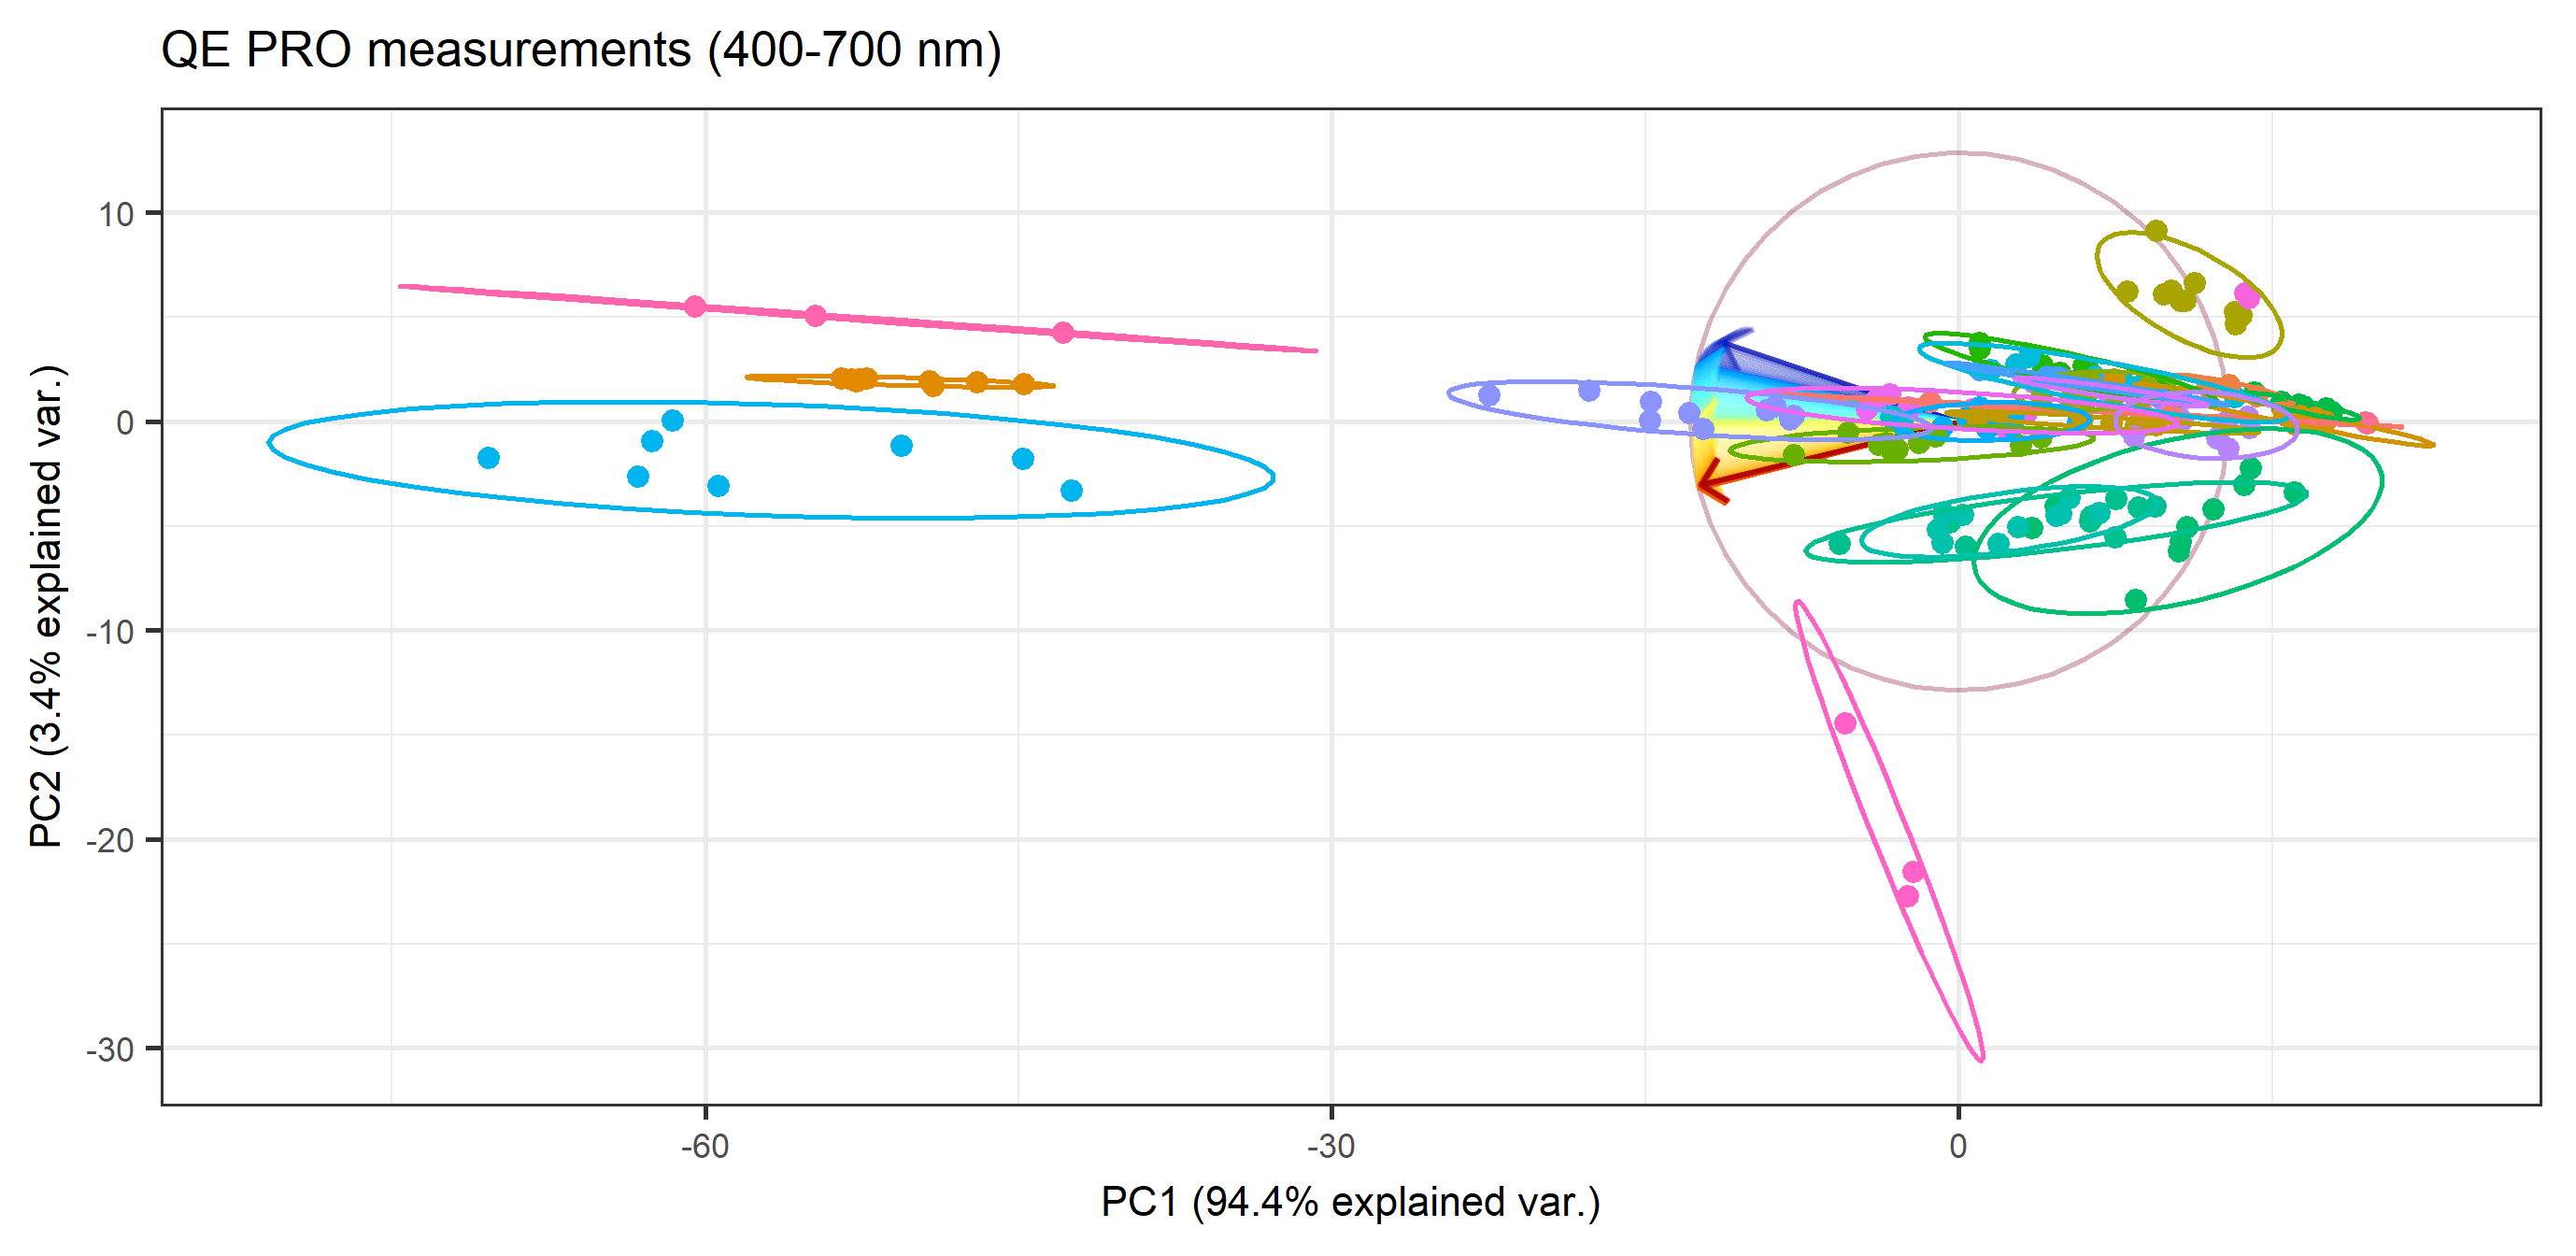
\includegraphics[width=1\textwidth]{Images/results/PCA_plastics_full_only_scat.png}
    \caption{Scatter plot of the results of the PCA with all plastic samples}
    \label{fig:PCA_plastics_only_full_scat}
\end{figure}


\begin{figure}[H]
   \centering
    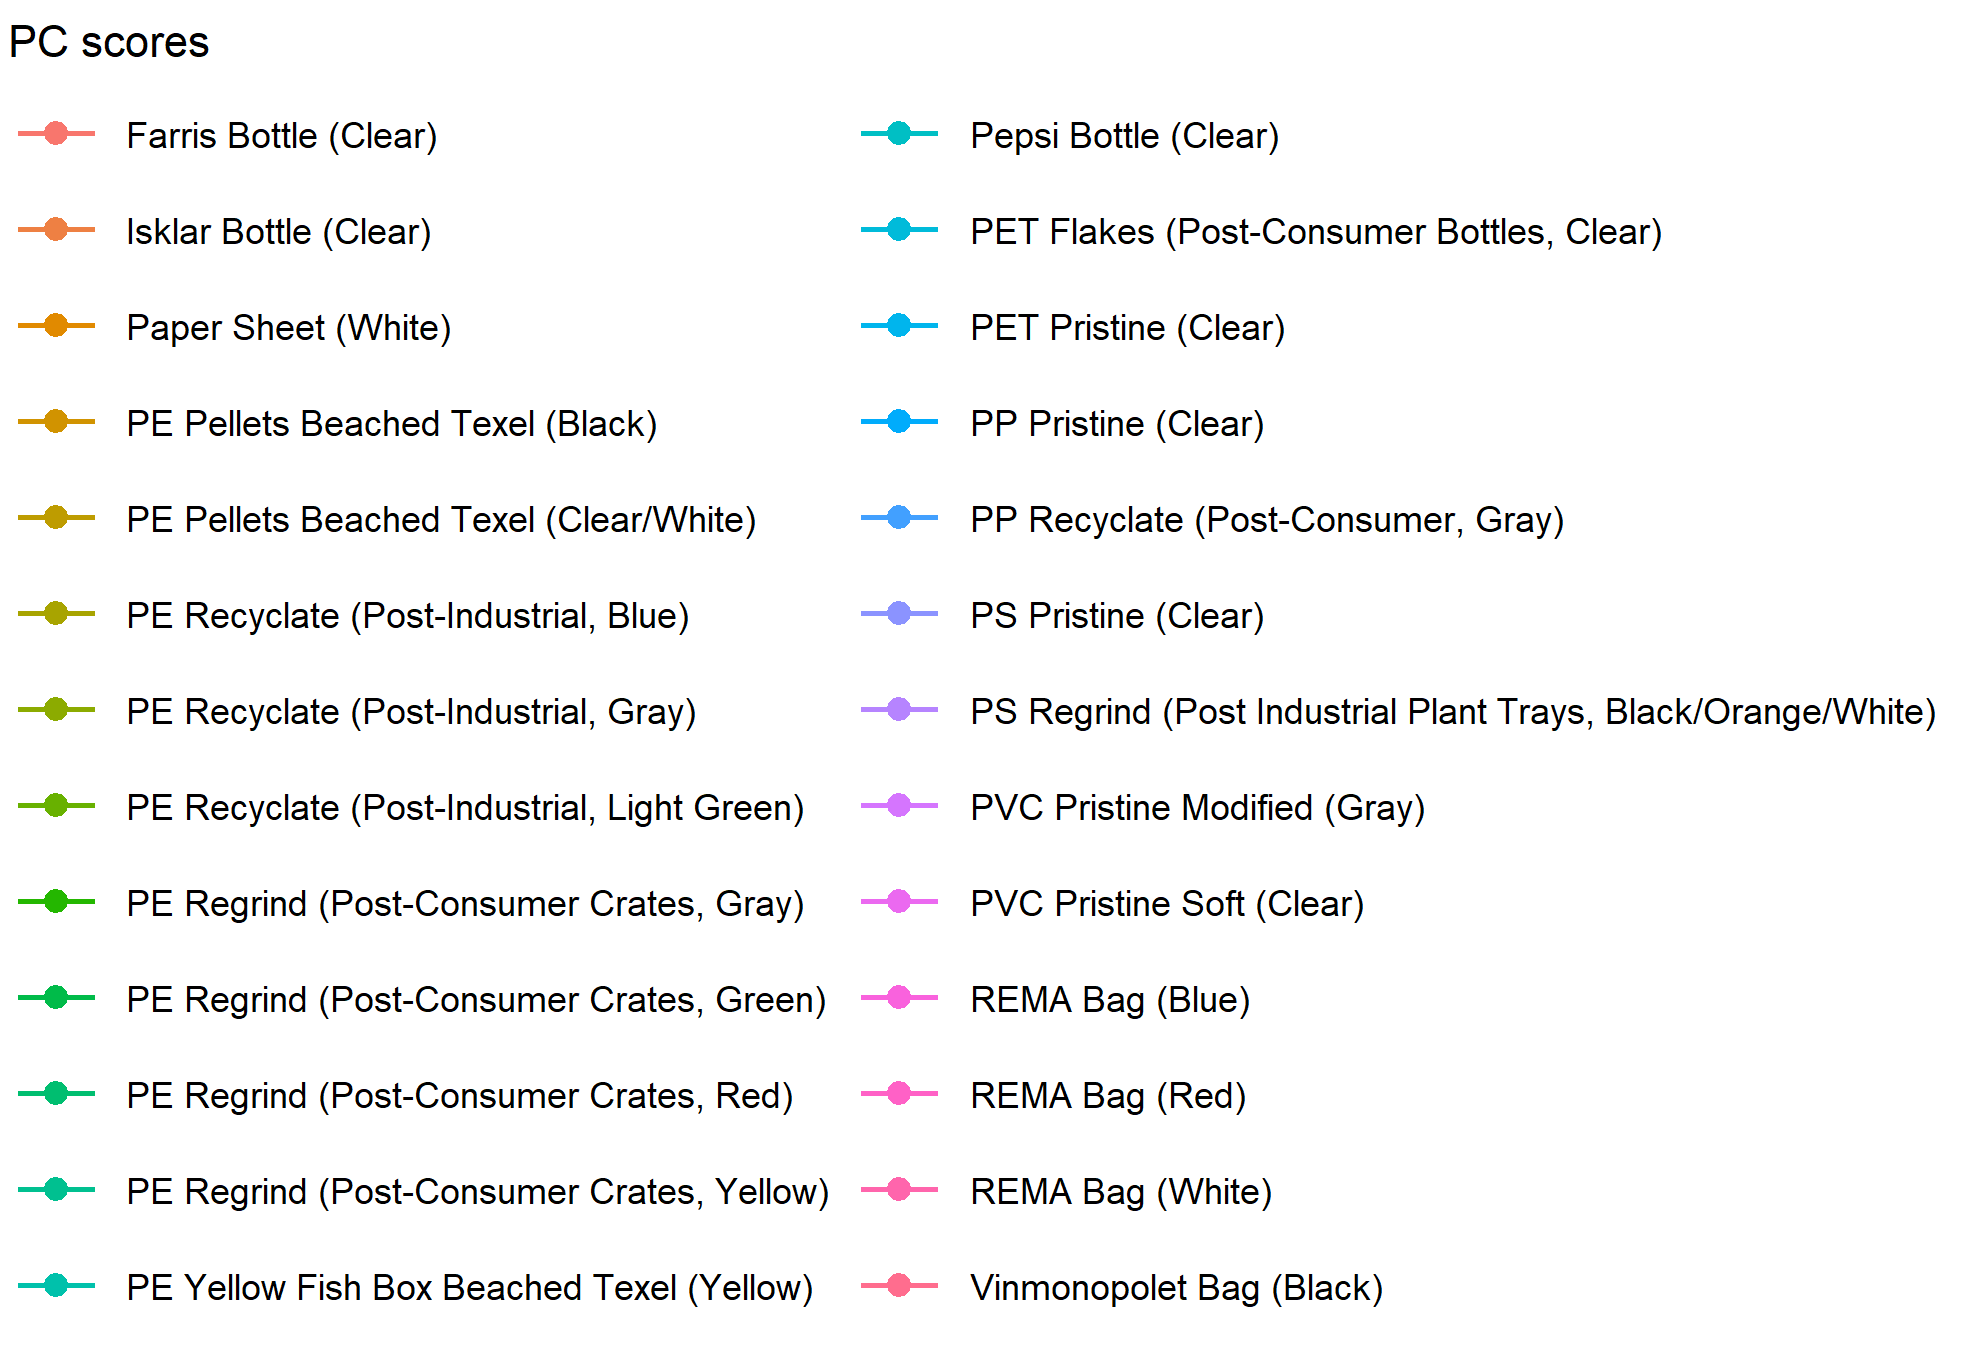
\includegraphics[width=0.7\textwidth]{Images/results/PCA_plastics_full_list.png}
  \caption{List of all scanned plastic samples and their respective colors.}
  \label{fig:PCA_plastics_full_list}
\end{figure}
\\\\
\noindent
As can be seen of the plot in Figure \ref{fig:PCA_plastics_only_full_scat}, PC1 accounts for over 94.1\% of the variance, while PC2 explains no more that 3.4\% of the variance. Interpreting the plot, there are three clustrings utenfor.. hvorfor? pga tynnhet og papiret. Velger å redusere ved å fjerne outliers vi ikke kan forklare fordi de har samme lyshet, farge og type som flere av de som ligger inne. Det resulterende sette, etter removal of outlying variables, presenteres i neste section.
\\\\
Figure \ref{fig:PCA_plastics_full_doub_cont} shows the contributions from the different wavelengths corresponding with the two principal components. The horizontal axis represent the wavelengths and the vertical axis the contribution in percent. The dashed red line represent 0.253\% or the line that shows the exact equal contribution from all wavelengths. Integrating the line would result in $0.253\% \cdot (700 - 400)/(0.758) \approx 100\%$.%Dette er feil. det skal være 0.252 siden det er en måling hver 0.758 og ikke hver nanometer, så er det mer riktig på bildet.
Also, the color of the line depicts the color at that wavelength, the blue color of the line at 450 nm is the color of light with that specific wavelength. 
\\\\%Påpeke at selv der man ser clusters så er ikke dette fremtredende i den samme plasttypen, men heller på bakgrunn av den fargen plasten innehar. 
\begin{figure}[H]
    \centering
    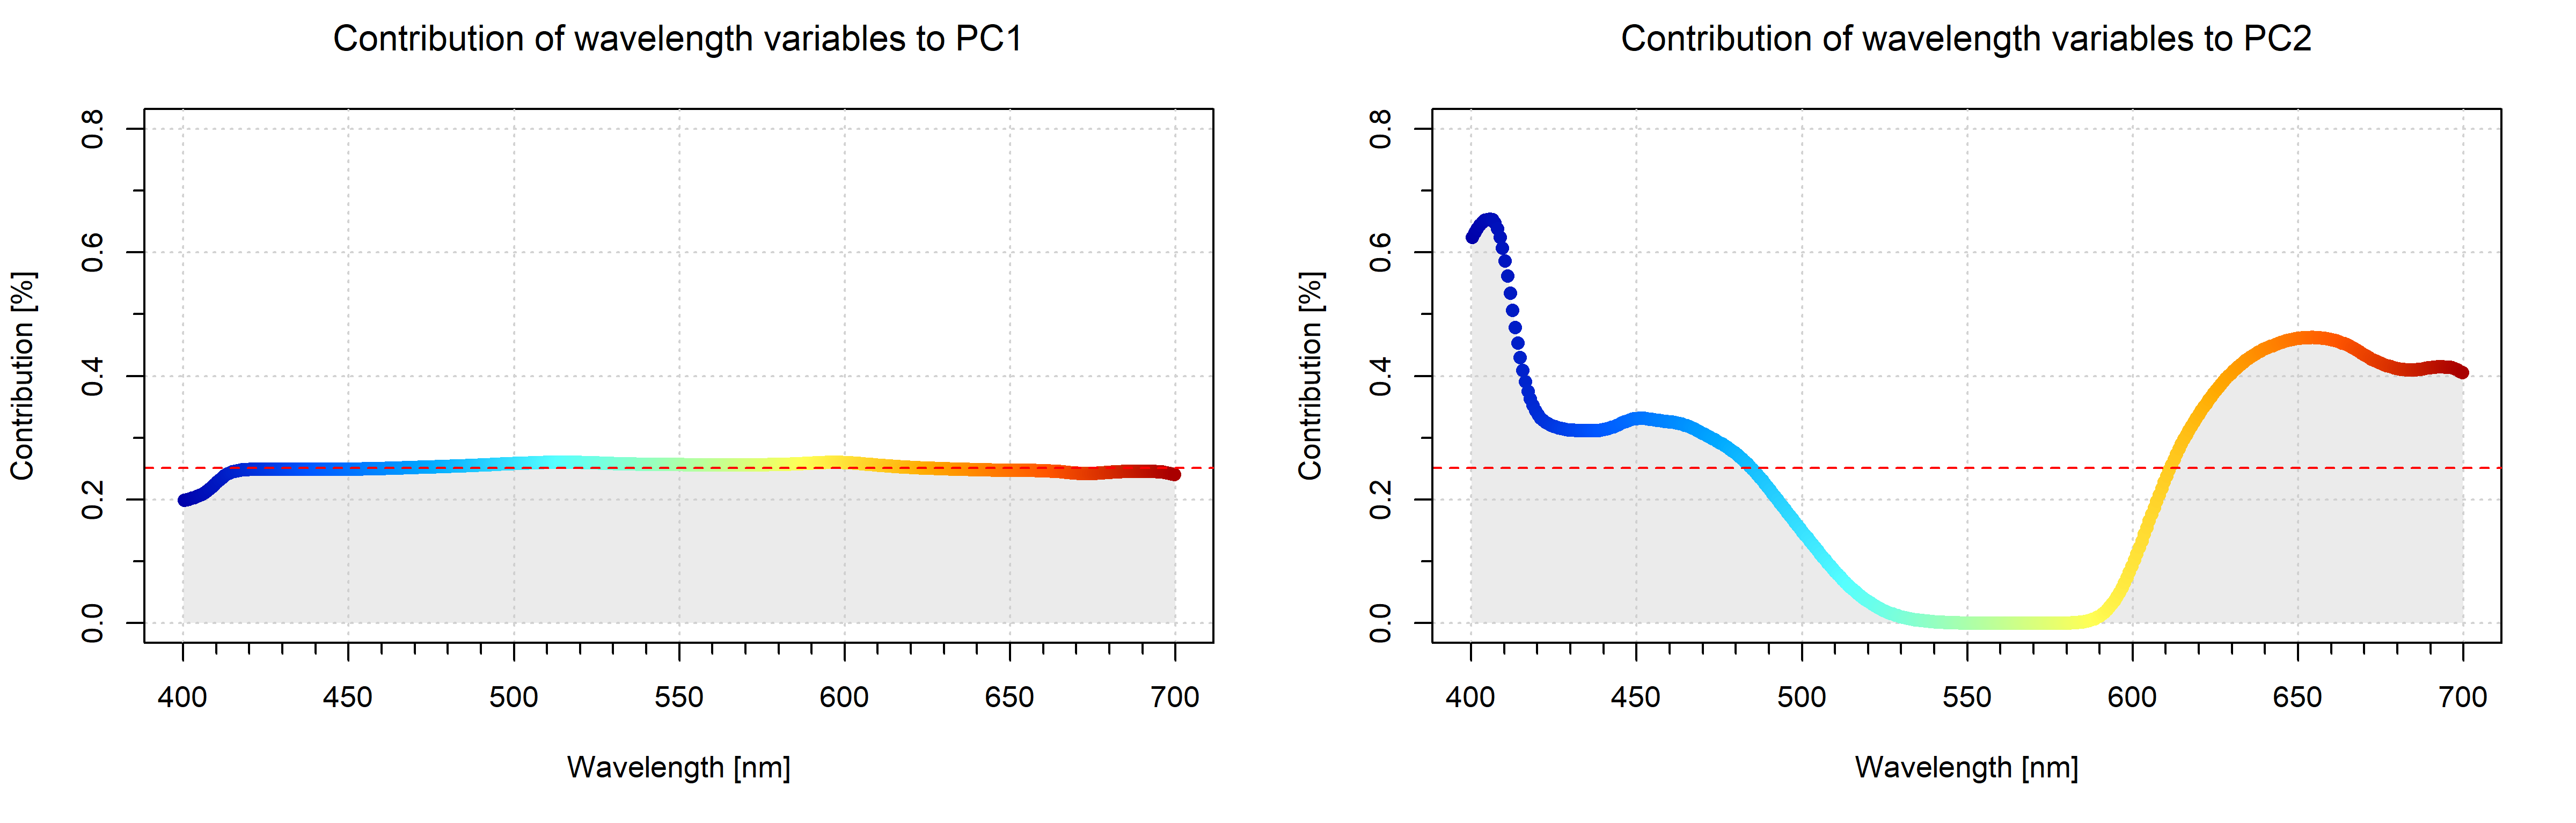
\includegraphics[width=1\textwidth]{Images/results/PCA_plastics_full_doub_cont.png}
    \caption{Contribution plot of the results of the PCA with all plastic samples.}
    \label{fig:PCA_plastics_full_doub_cont}
\end{figure}
\noindent
From the signature and contribution of PC1 in Figure \ref{fig:PCA_plastics_full_doub_cont} it is apparent that the 94.1\% descriptive property of the first principal component is not rooted in one wave length or in a combination of wavelengths. The even distribution over the spectrum visualize the fact that PC1 mainly describes the \textit{lightness} of the plastic. 
\\\\
In addition, the position of the different samples in Figure \ref{fig:PCA_plastics_only_full_scat}, also indicate that the results are dominated by this fact. Due to the low variance of the second principal component, of only 3.4 \%, the vertical spread and thus the few clusters there are, are not well described and may not be deemed representative.
\\\\

\subsection{Principal Component Analysis with Reduced Plastic Samples}
As explained in the previous section, the results presented in this section are from a reduced dataset. Based on the knowledge provided through analyzing the results of the full set, some variables was removed. This way, the reduced set contains only relevant redeemed variables without wrongly measured samples possibly pulling the result in the wrong direction. 
\\\\
Figure \ref{fig:PCA_plastics_reduced_only_scat} is the scatter plot describing this reduced set. The properties of this scatter plot are the same as for the scatter plot presented for Figure \ref{fig:PCA_plastics_only_full_scat} in Section \ref{sec:pcafull}, and will therefore not be elaborated here as well.

\begin{figure}[H]
    \centering
    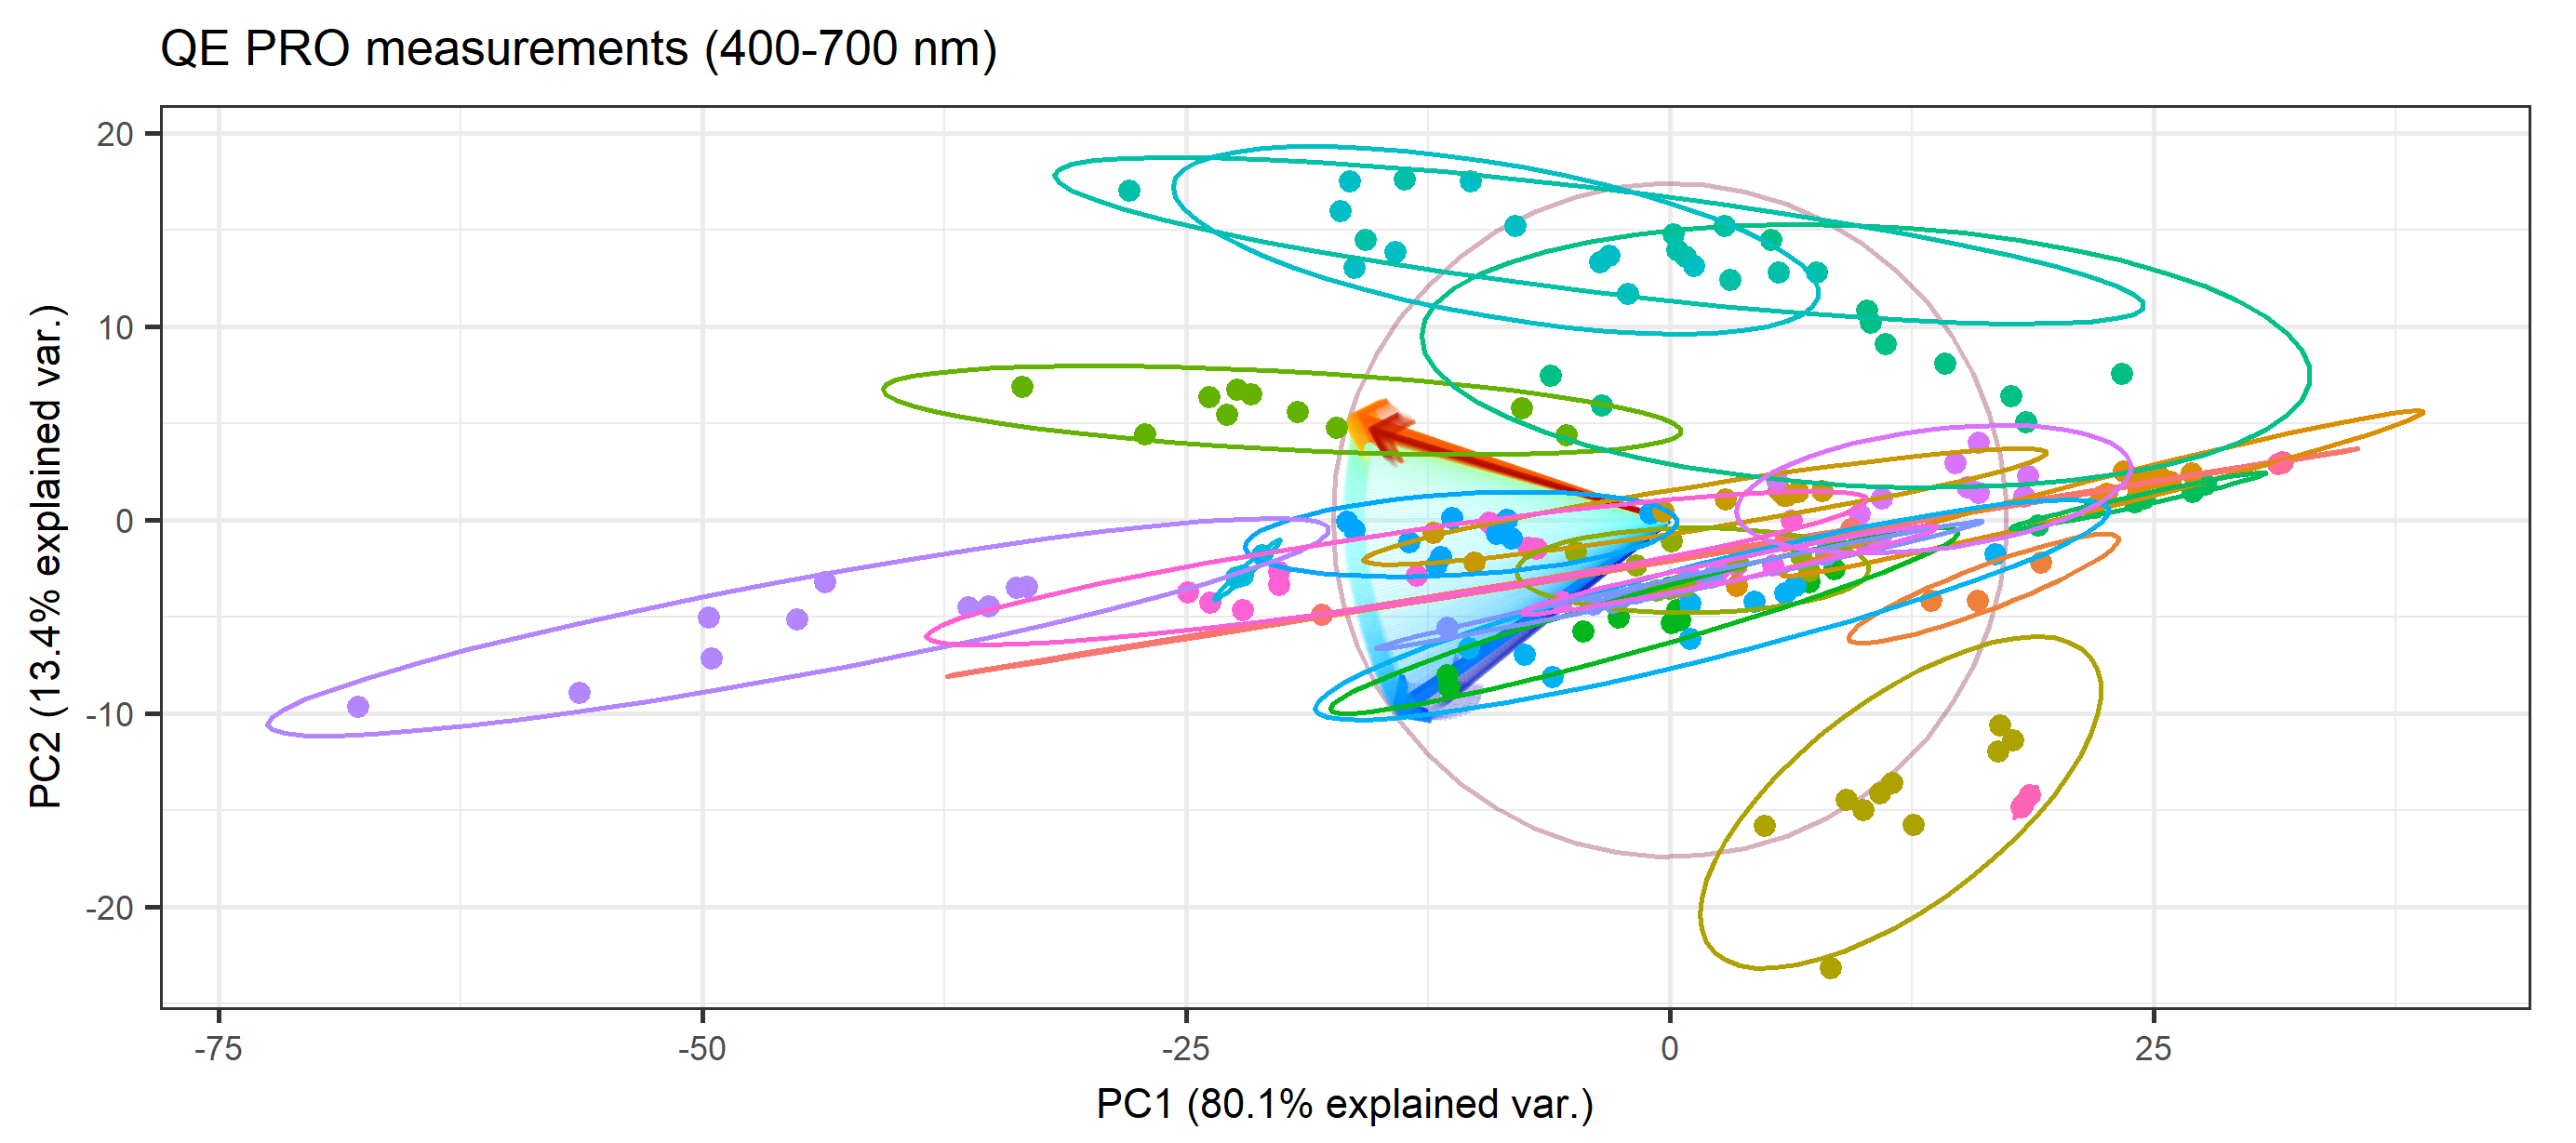
\includegraphics[width=1\textwidth]{Images/results/PCA_plastics_reduced_only_scat.png}
    \caption{Results of the PCA with reduced Plastic Samples}
    \label{fig:PCA_plastics_reduced_only_scat}
\end{figure}

\begin{figure}[H]
    \centering
    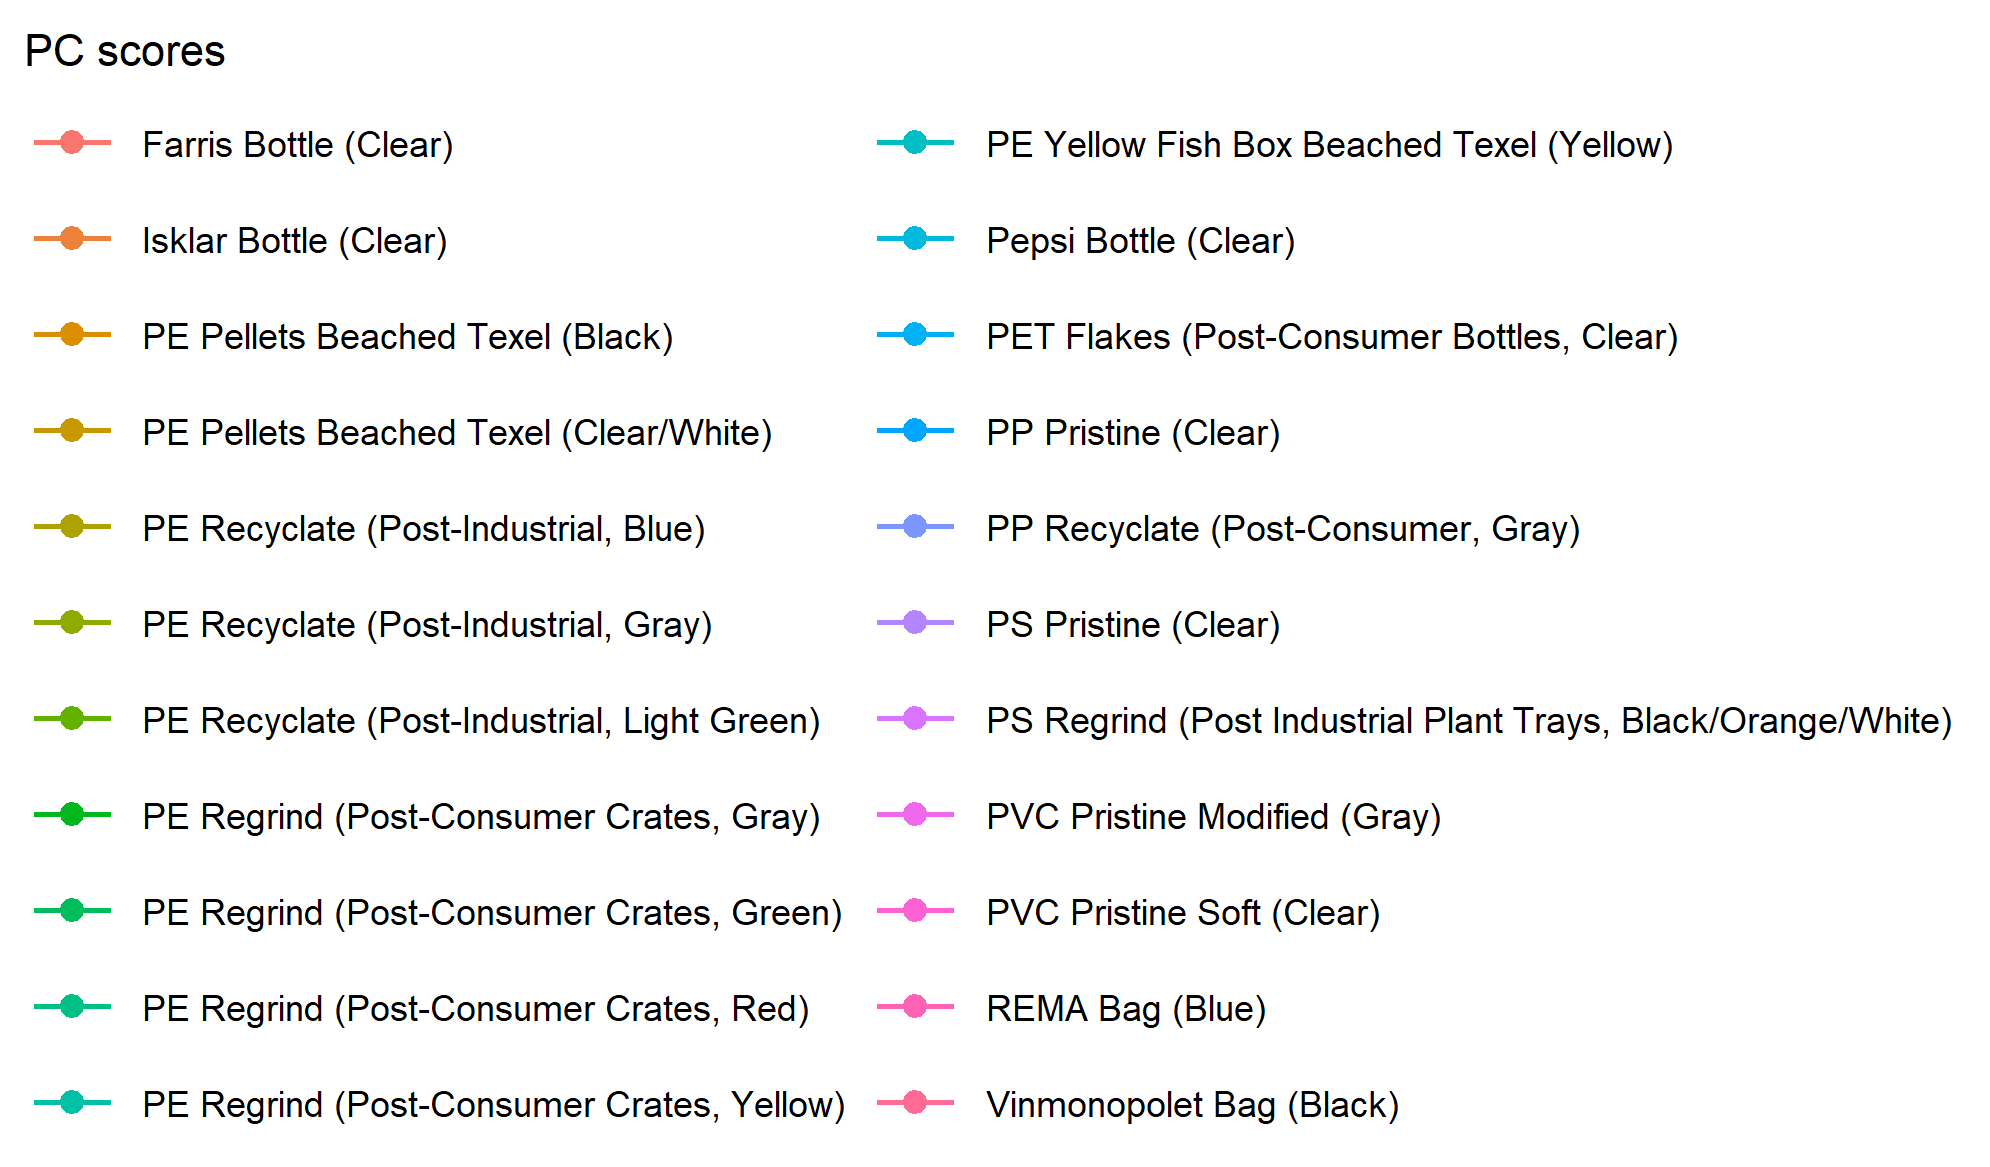
\includegraphics[width=0.7\textwidth]{Images/results/PCA_plastics_reduced_list.png}
    \caption{List of the reduced scanned plastic samples and their respective colors.}
    \label{fig:PCA_plastics_reduced_list}
\end{figure}
\noindent
PC1 now represents 80.1\% of the variance, while PC2 explains 13.4\% of the variance. Despite the lower explanation percentage of PC2, there are clusters. These are quite apparent in the top and bottom of the scatter plot (\ref{fig:PCA_plastics_reduced_only_scat}). The issue arise when comparing these clusters to their respective plastic type. There are no other clear clusters related to these types of plastic. In fact, it seems that the clear clusters these types are a part of, are based on the color of the plastic, not inherent properties of the material. The bottom cluster consists of PE Recyclate of the color blue together with samples retrieved from the blue part of the logo on a plastic bag. Similarly, the top cluster consists of PE Regrind and PE Yellow Fish Box Beached Texel, both of which are yellow-colored. It is therefore difficult to argue that these clusters indicate anything other than the color additives in the material.
\\\\
%Tenke på å markere clusterene med tall, slik at det blir lettere å omtale
Based on the tendency of the clear plastic to be on the left side of the cluster, one can assume that the white paper background have had an impact on the results, and subsequently on the principal components. The samples of PS Pristine were particularly clear, as may be seen from the table in the Section \ref{sec:material} in Chapter \ref{chap:method}, or as an image in Appendix \ref{app:image_plast}. Given that these are the main contributions to the spread along the horizontal axis, one could argue that without the light background, the lightness and clearness of the material would be less prominent in the first principal component. This would possibly further change the composition of the principal components and subsequently change the patterns on the scatter plots. 
\\\\%Snakke med Asgeir om dette og høre hva han tenker om at papiret har påvirket resultatene og at vi i utgangspunktet ikke har tid til å tilbringe en hel ny dag på laben for å teste på nytt. Aksel har gjort tester tidligere der han har fått samme resultat med at "lysheten" til prøvene har hatt stor innvirkning
\noindent
The associated contribution plot is displayed in Figure \ref{fig:PCA_plastics_doub_cont}. This plot show how the different wavelength contribute in correspondence to PC1 and PC2, respectively. 

\begin{figure}[H]
    \centering
    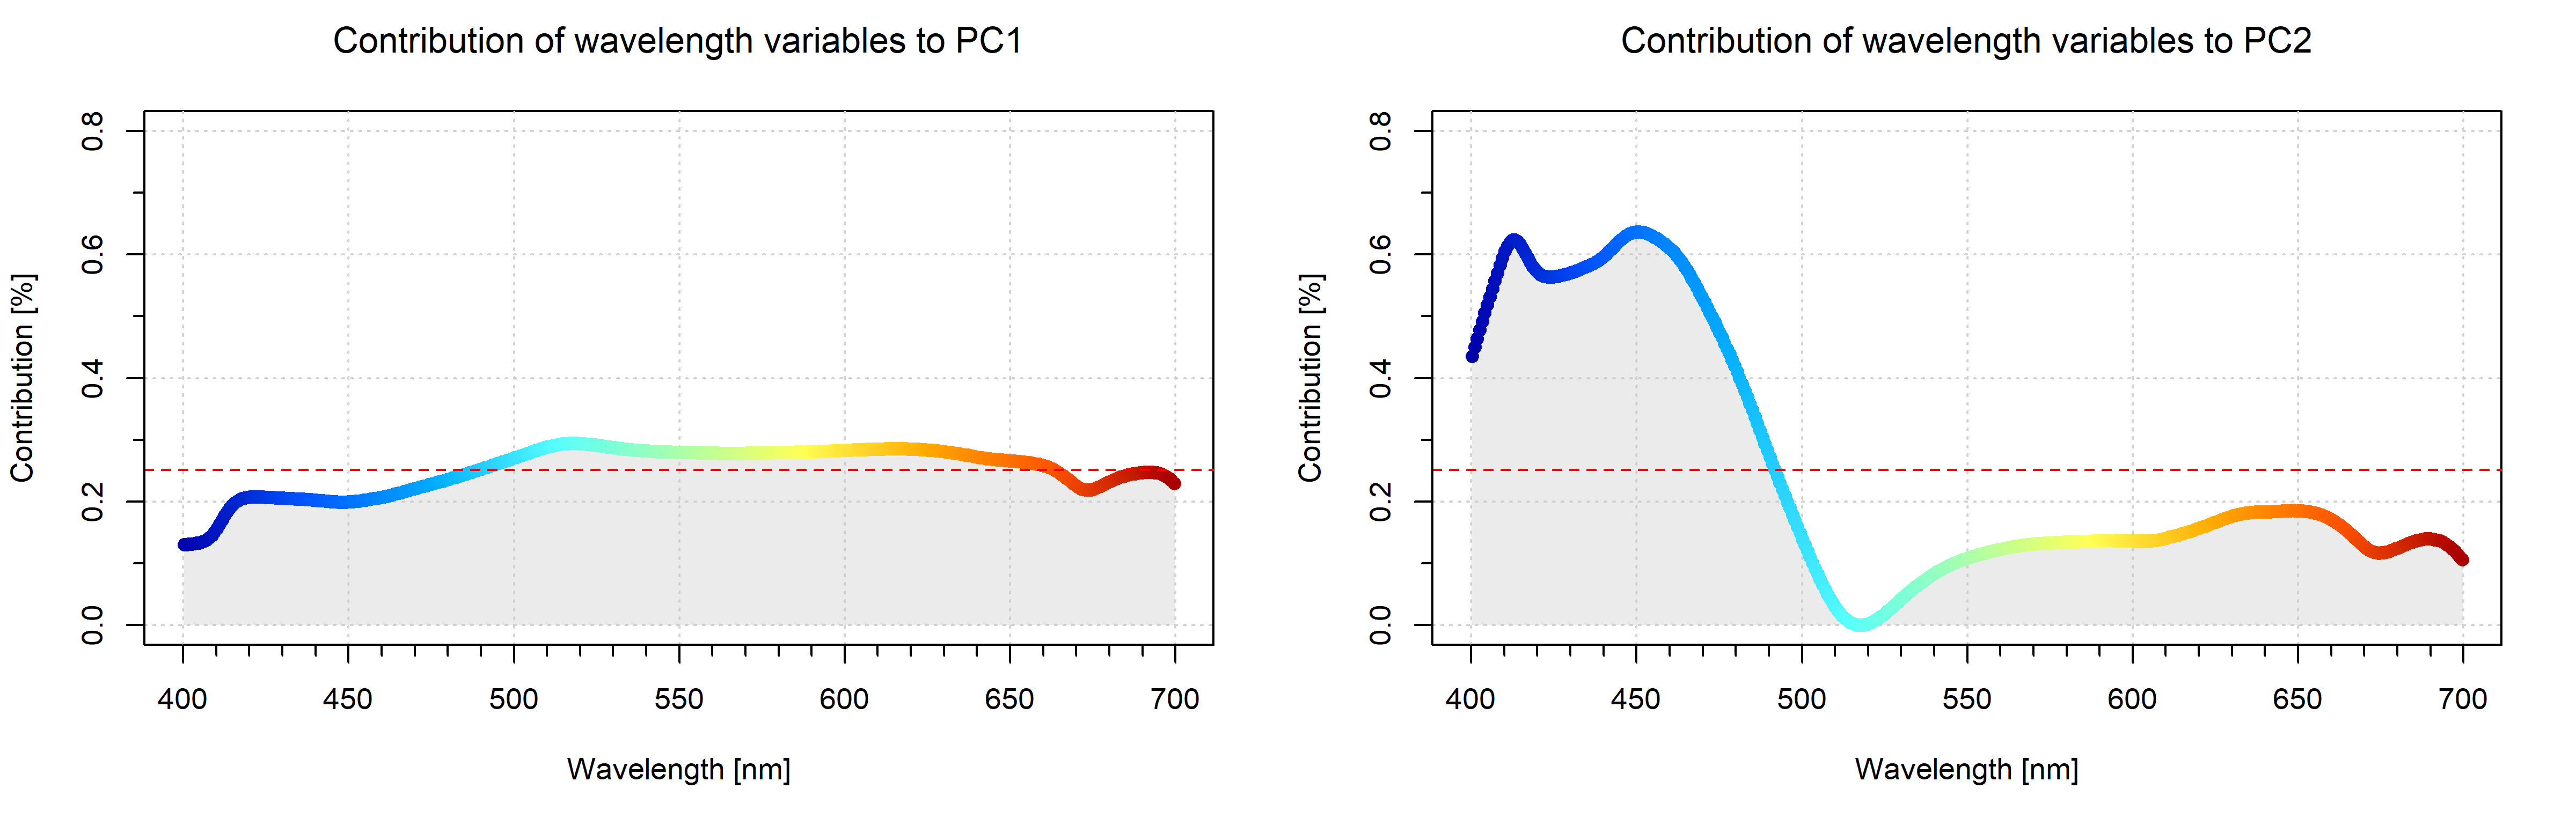
\includegraphics[width=1\textwidth]{Images/results/PCA_plastics_reduced_doub_cont.png}
    \caption{Contribution plots of the two principal components of the PCA with reduced plastic samples}
    \label{fig:PCA_plastics_doub_cont}
\end{figure}
\noindent
The contribution plot of the second principal component imply that the lower end of the spectrum has ha larger impact than the larger wavelengths. 

\subsection{Principal Component Analysis with Biological Components}
Figures \ref{fig:PCA_plastics_and_biology_scat} and \ref{fig:PCA_and_bio_cont_plots} are plots describing the results of plastic samples together with biological pigments - initially presented at the end of Chapter \ref{chap:method}. These plots have the same properties as those above, solely consisting of plastic.

\begin{figure}[H]
    \centering
    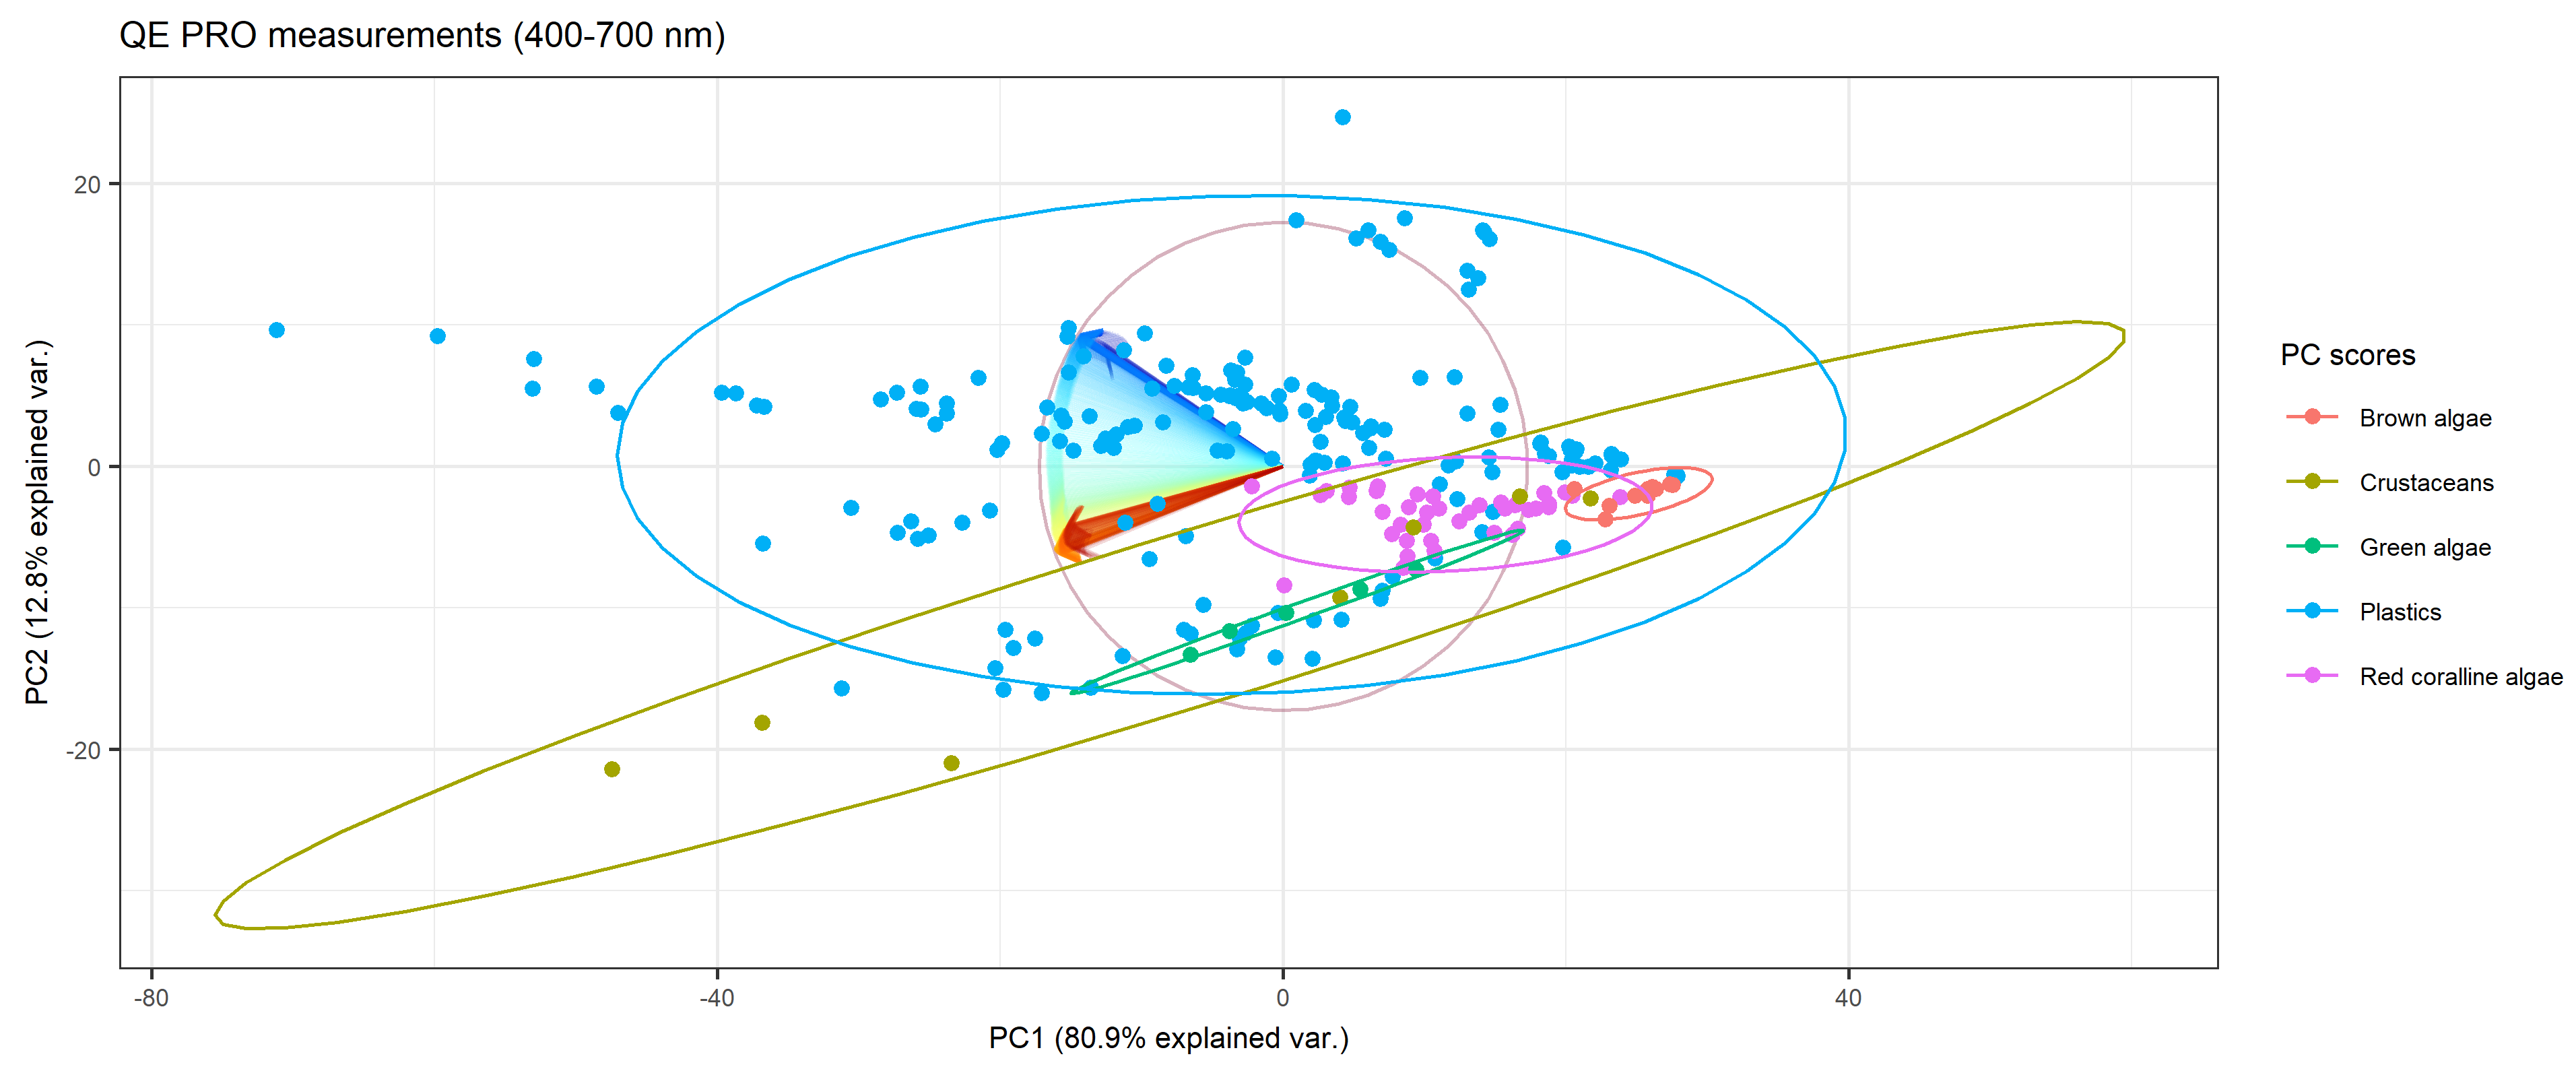
\includegraphics[width=1\textwidth]{Images/results/PCA_plastics_and_biology_scat_clust.png}
    \caption{Results of the PCA with Plastics and Biological Components}
    \label{fig:PCA_plastics_and_biology_scat}
\end{figure}


\begin{figure}[H]
  \newcommand*\FigVSkip{0.5em}
  \newcommand*\FigHSkip{0.1em}
  \newsavebox\FigBox
  \centering
  % Top image is centered, so no need to get width
 \sbox{\FigBox}{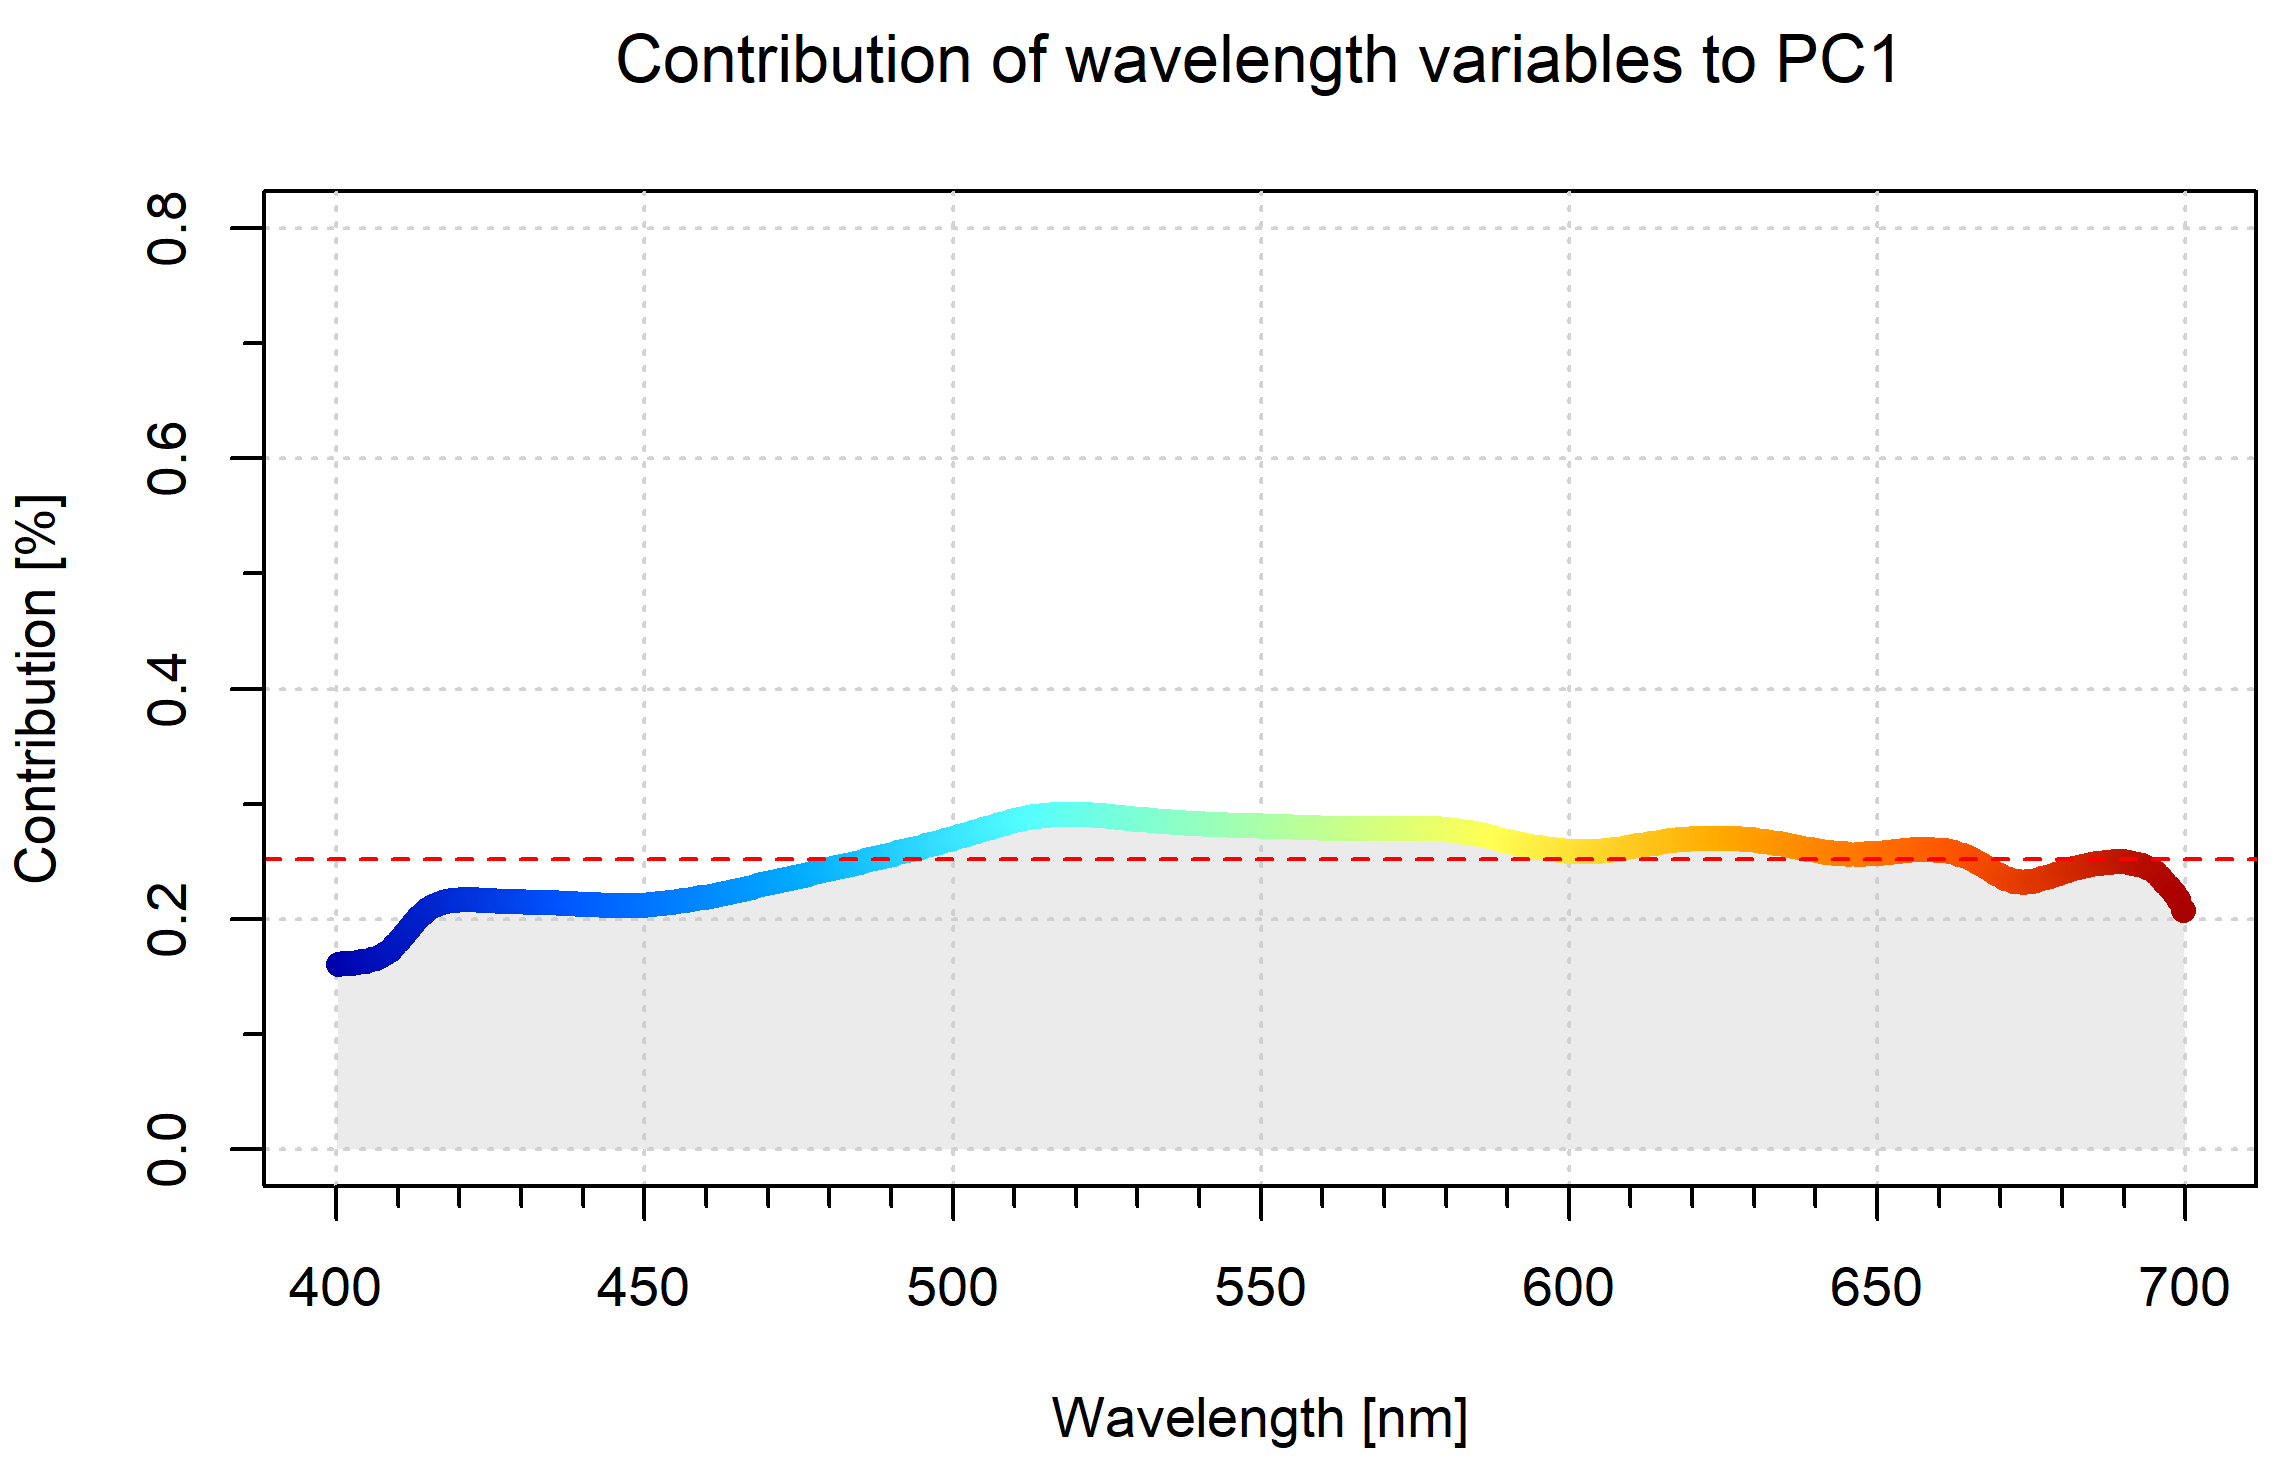
\includegraphics[scale=0.5]{Images/results/PCA_plastics_and_biology_cont_pc1.png}}
  \begin{minipage}{\wd\FigBox}
    \centering\usebox{\FigBox}
     \label{fig:PCA_plastics_and_biology_cont_pc1}
  \end{minipage}
    % Top image is centered, so no need to get width
 \sbox{\FigBox}{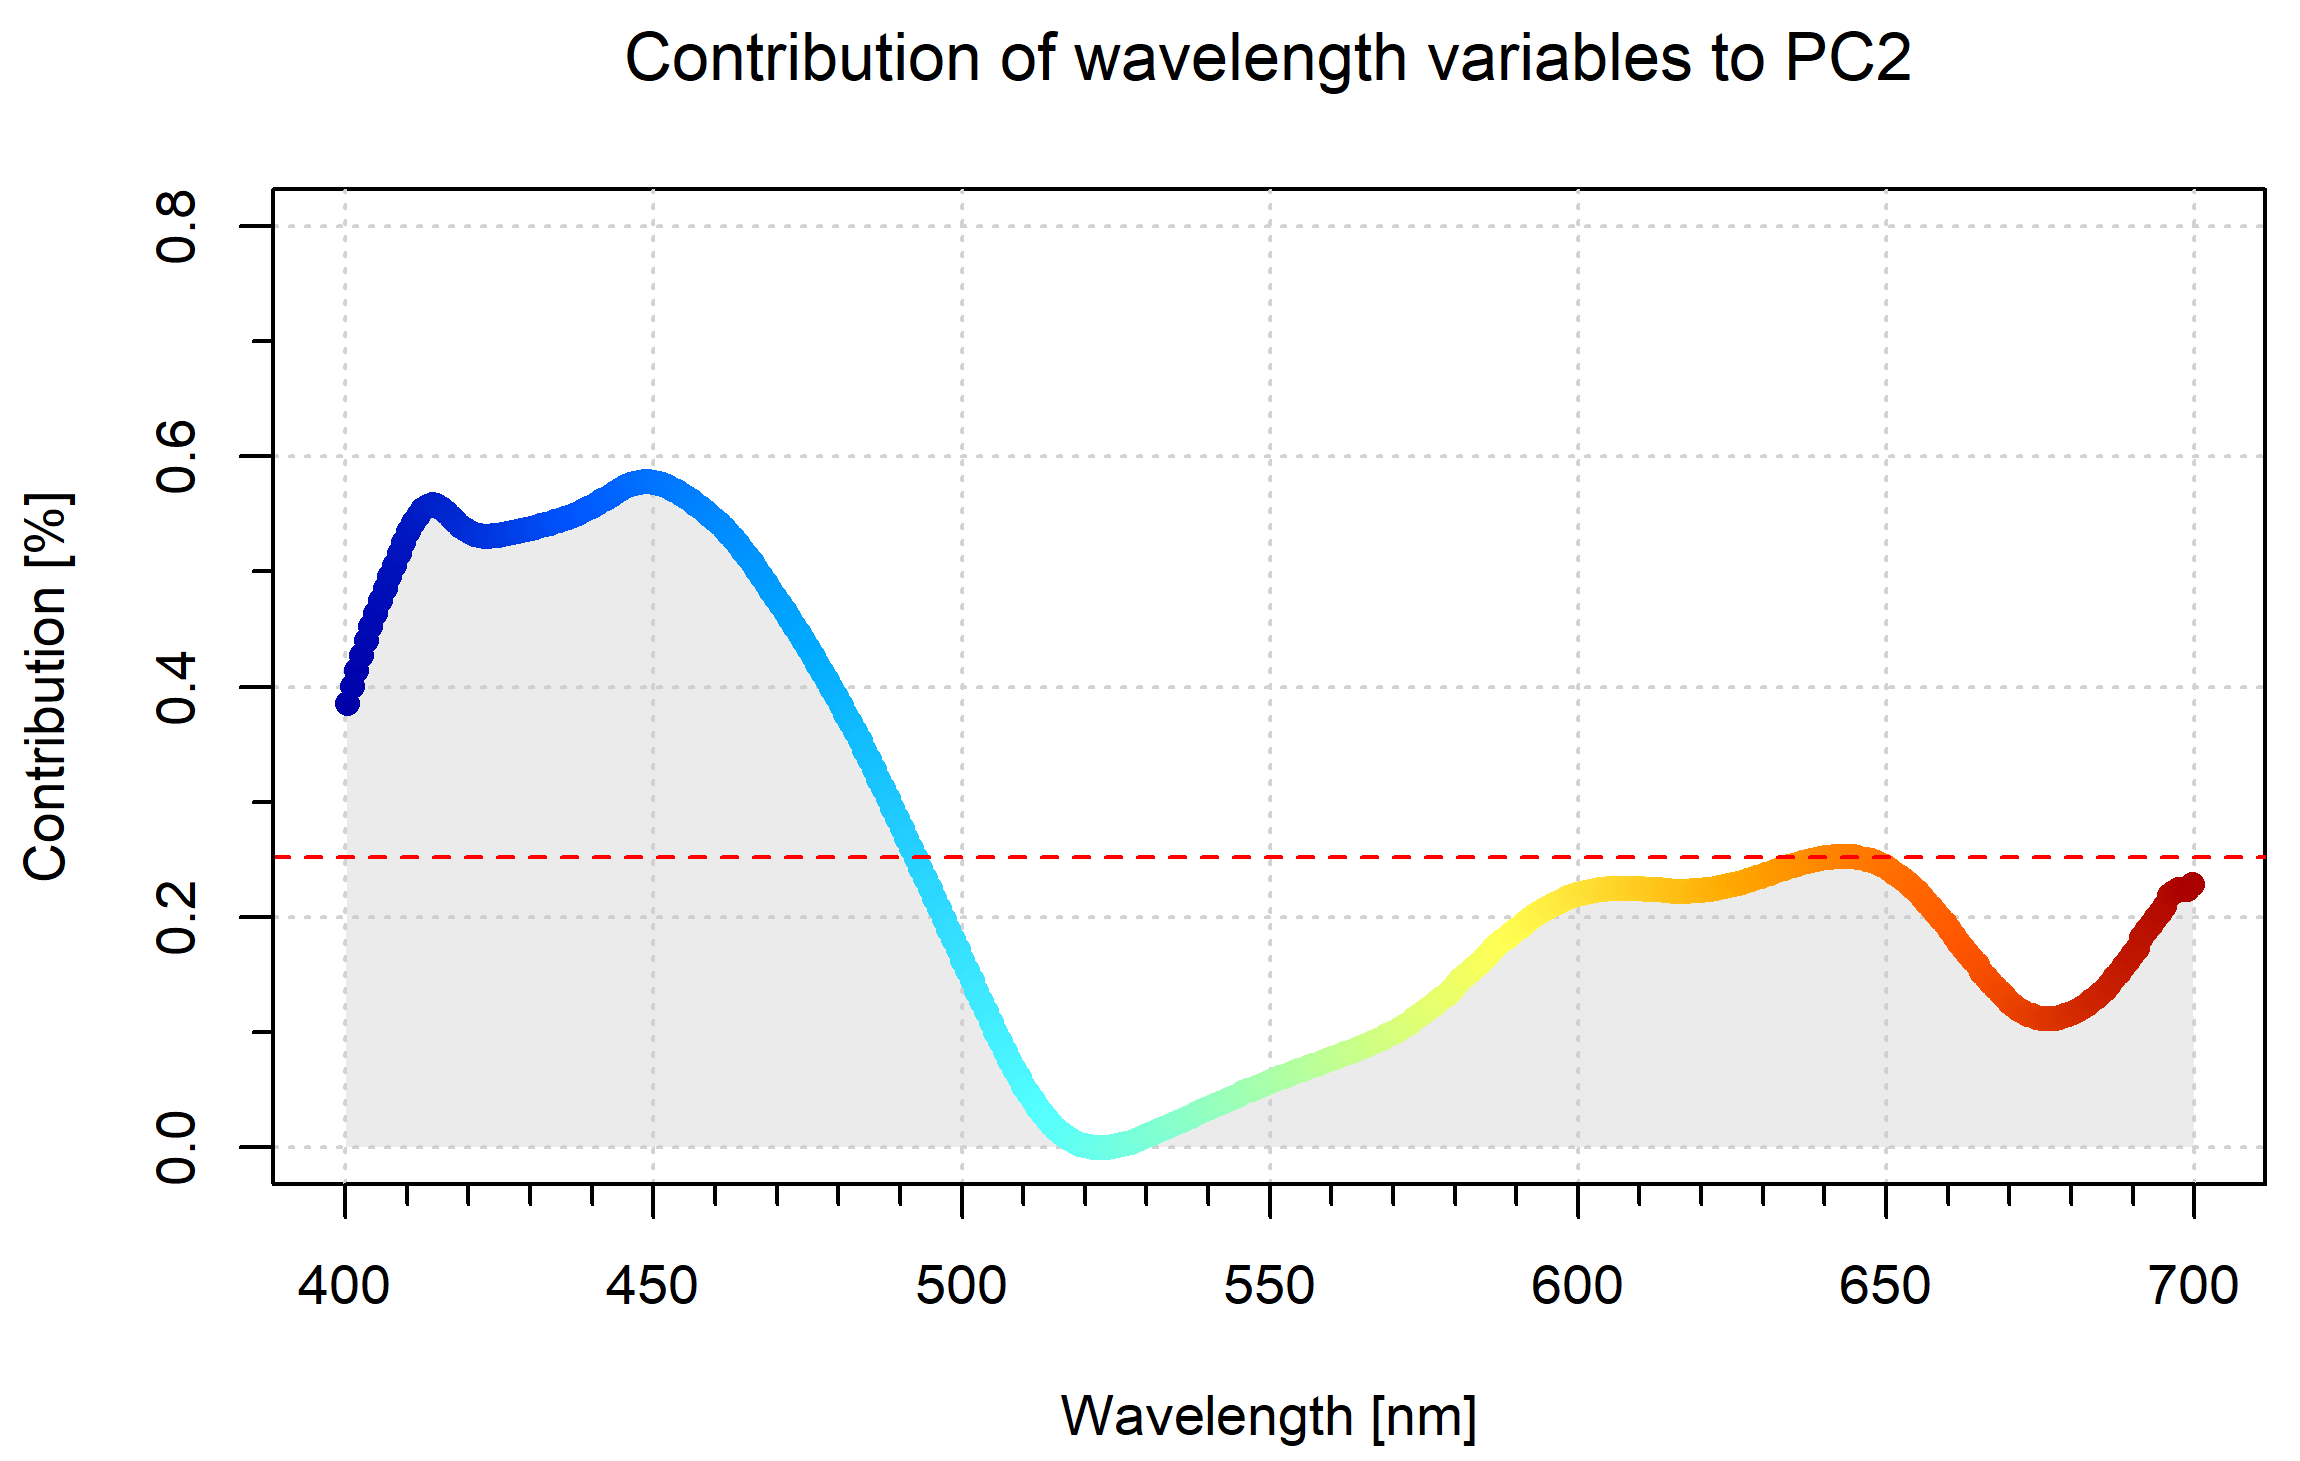
\includegraphics[scale=0.5]{Images/results/PCA_plastics_and_biology_cont_pc2.png}}
  \begin{minipage}{\wd\FigBox}
    \centering\usebox{\FigBox}
  \label{fig:PCA_plastics_and_biology_cont_pc2}
  \end{minipage}
  % Save second image 
  \caption{Contribution plots for the PCA with plastic and biological samples}
\label{fig:PCA_and_bio_cont_plots}
\end{figure}
\noindent
Interpreting these figures, a more prominent trend became apparent. The natural occurring pigment in algae and crustaceans differed from the plastic in the scatter plot. This shows potential for distinguishing plastic in general from organic pigments naturally occurring in the marine environment.
\\\\%Argumentere med at her ser man at den klare plasten ligger utenfor konfidens intervallet og kan dermed mulig ekskluderes i en ny runde med forsøk, eventuelt at man endre bakgrunnen slik at den ikke er hvit og dermed ikke påvirker lysheten i tilsvarende grad. 
The contribution on the first principal component does not differ much from the associated components in the previous plots. However, given the mentioned effect of the clear plastic, this might change with the use of a less reflective background. Furthermore, in Figure \ref{fig:PCA_plastics_and_biology_scat} all plastic samples are gathered in one confidence interval ring. The result is that the previously mentioned clear plastic lies outside the confidence interval. This would further underline the previous suspicion that there is a prominent effect from the white background on the results.
\\\\
Experience has shown that the brightness/lightness of the samples is highly relevant also when not investigating plastic. Therefore, the change in background might affect the results, but it is not expected to revolutionize them.
\\\\\\
Now, what can be drawn of this? Acquiring distinct signatures for the specific types of plastic, seems unlikely using a hyperspectral image. Neither was is possible to find a general signature for the plastic, increasing the difficulty of detecting plastic as a total. %which could be used as an end-member or for Spectral Angle Mapping. 
\\\\
Despite seeing a resemblance of a signature in the second principal component it is important to keep in mind the components do not represent actual signatures. They rather depict the wavelengths which have a larger influence on the vertical distinguishing of the samples.
\\\\
Based on the absence of clear clusters it was deemed not possible to acquire what is thought of as unique signatures for the plastic. All three analyses do show vertical spread, but the large number of overlapping samples made it difficult to argue for the existence of clear signatures at this stage. In the analysis with the presence of the organic pigments, there are some indication of separation, but not enough argue for a general signature for the plastic. However, the clustering seen in the sample does pose an opportunity of distinguishing plastic from the natural occurring pigments. 

\vspace{1.3cm}
\section{Signatures}

\subsection{Constant Color}
The resulting signatures were highly affected by the color of the targeted plastic pellets. Figure \ref{fig:plastcomp1}, shows the spectrum of two types, PP and PVC respectively. 

\begin{figure}[H]
  \newcommand*\FigVSkip{0.5em}
  \newcommand*\FigHSkip{0.1em}
  \newsavebox\FigBox
  \centering
  % Top image is centered, so no need to get width
 \sbox{\FigBox}{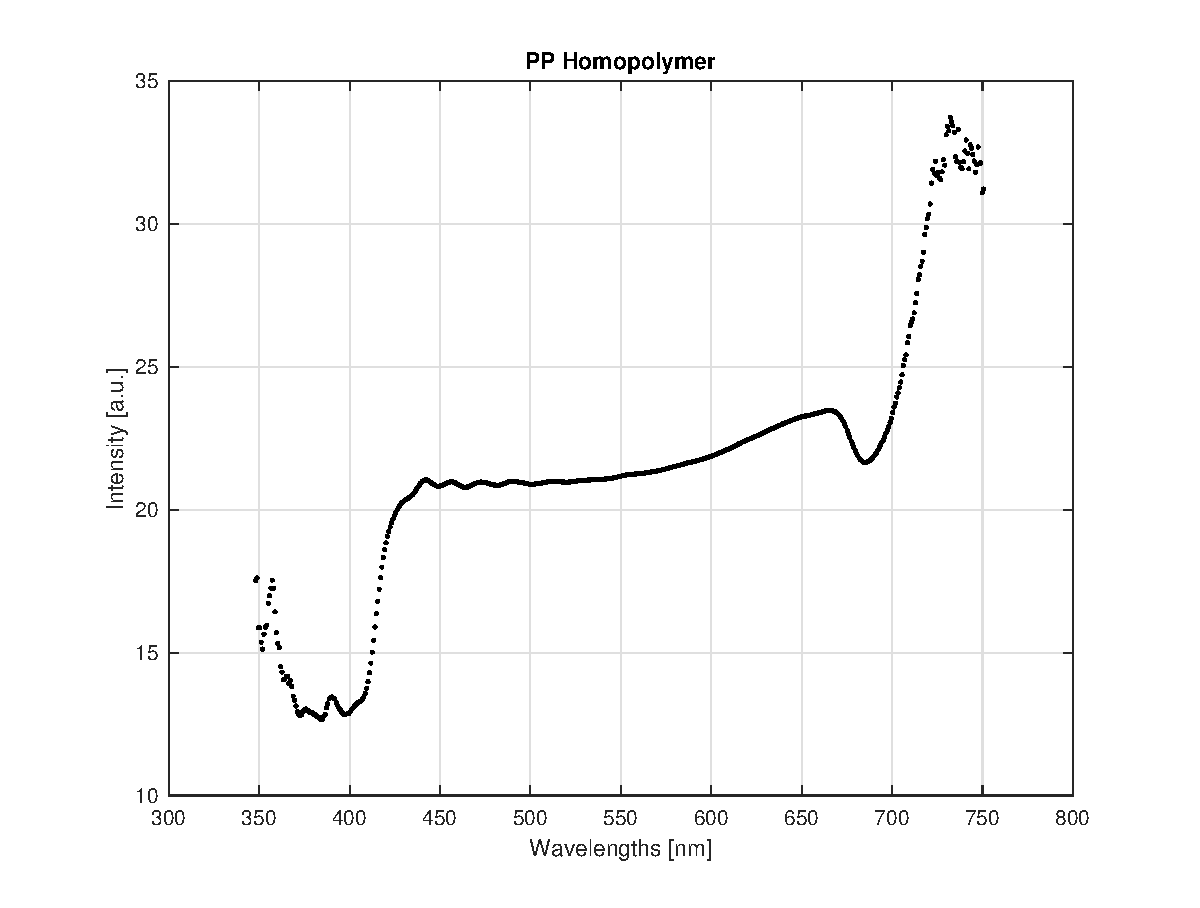
\includegraphics[scale=0.36]{Images/appendix/pp-pristine-clear.eps}}
  \begin{minipage}{\wd\FigBox}
    \centering\usebox{\FigBox}
    \subcaption{a) PP Pristine}
  \end{minipage}
    % Top image is centered, so no need to get width
 \sbox{\FigBox}{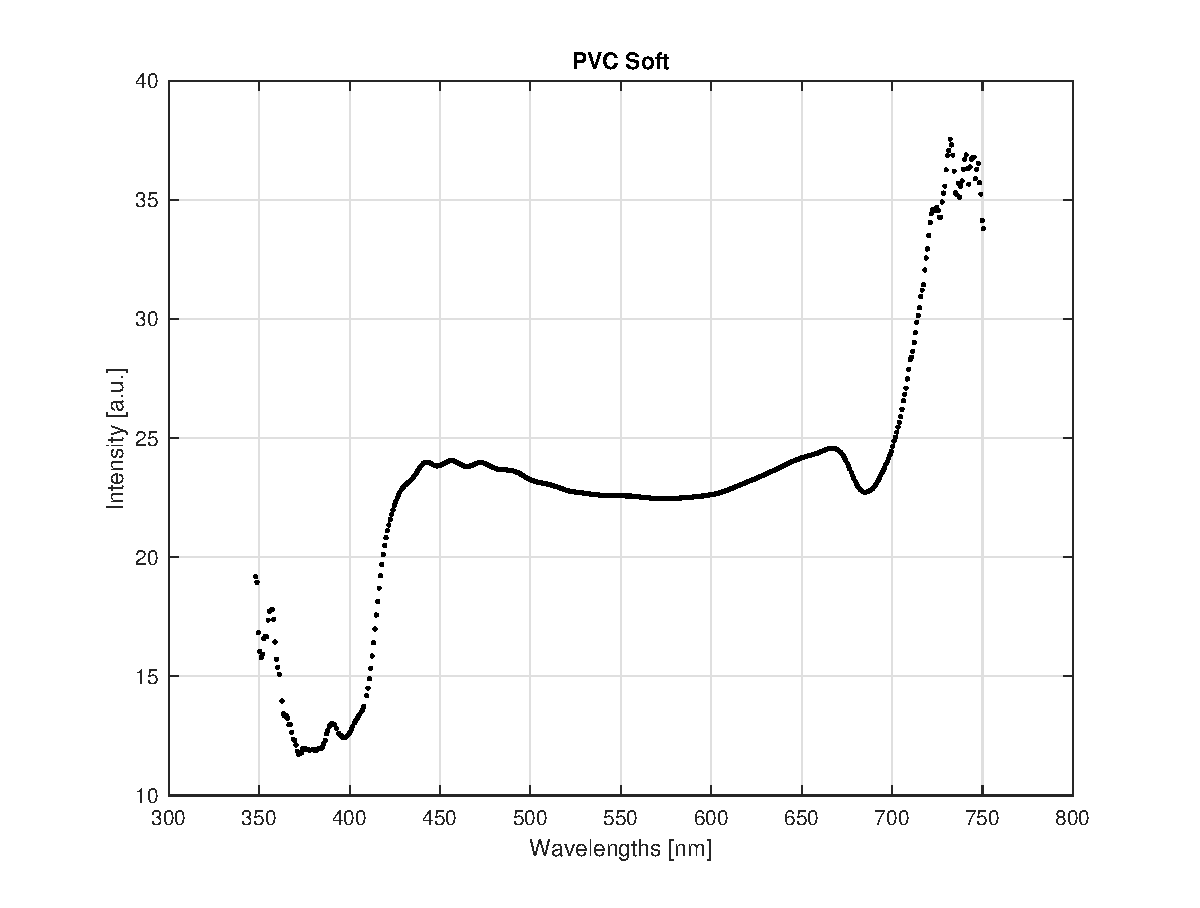
\includegraphics[scale=0.36]{Images/appendix/pvc-soft-pristine-clear.eps}}
  \begin{minipage}{\wd\FigBox}
    \centering\usebox{\FigBox}
    \subcaption{b) PVC Soft Pristine}
  \end{minipage}
  % Save second image 
  \caption{A comparison of the resulting signature for PP and PVC - both clear-colored}
  \label{fig:plastcomp1}
\end{figure}

%denne viser gule for pe og pe-hd, men de er kanskje for like..
\begin{comment}
\begin{figure}[H]
  \newcommand*\FigVSkip{0.5em}
  \newcommand*\FigHSkip{0.1em}
  \newsavebox\FigBox
  \centering
  % Top image is centered, so no need to get width
 \sbox{\FigBox}{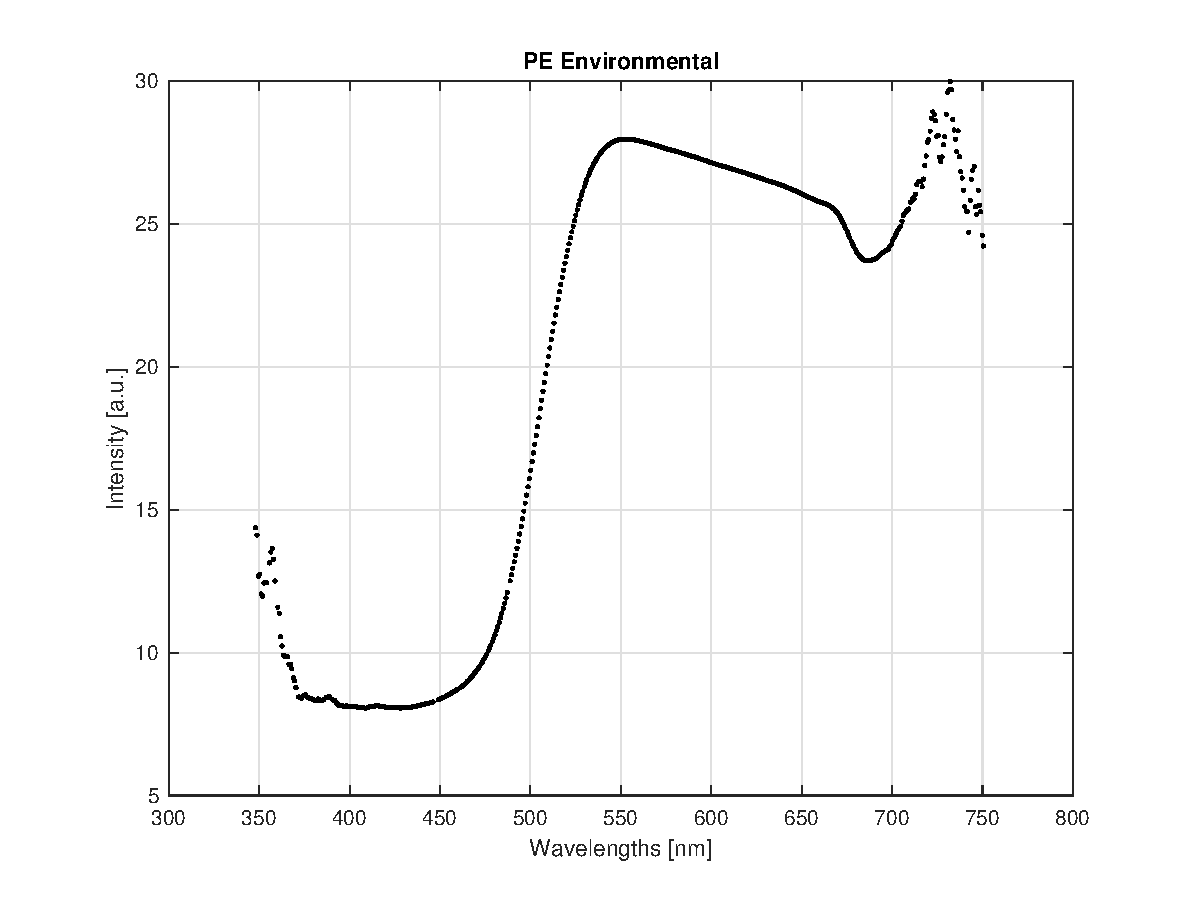
\includegraphics[scale=0.36]{Images/appendix/p-env_yellowbowl.eps}}
  \begin{minipage}{\wd\FigBox}
    \centering\usebox{\FigBox}
    \subcaption{a) PE Environment}
  \end{minipage}
    % Top image is centered, so no need to get width
 \sbox{\FigBox}{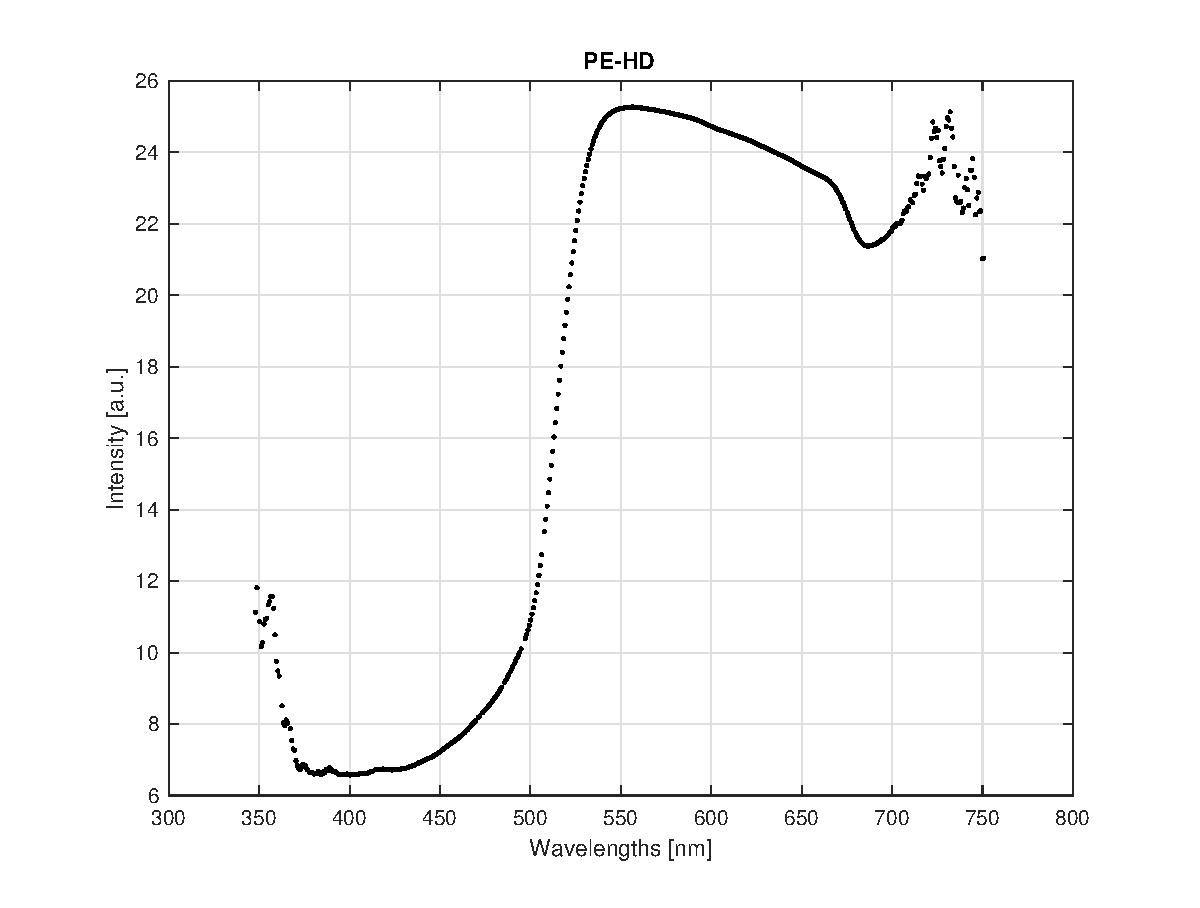
\includegraphics[scale=0.36]{Images/appendix/pe-hd-postconsum.eps}}
  \begin{minipage}{\wd\FigBox}
    \centering\usebox{\FigBox}
    \subcaption{b) PE-HD Post Consumer}
  \end{minipage}
  % Save second image 
  \caption{A comparison of the resulting signature for  and PVC - both in a yellow color}
  \label{fig:plastcomp1}
\end{figure}
\end{comment}


\noindent
As can be seen from Figure \ref{fig:plastcomp1}, the signatures of the two types are almost identical, with a possibility of deviations due to measurements errors. From Section \ref{sec:microplastic}, we know for a fact that the structure of these two are very different. PP contains several molecules with the chemical formula of $C_3H_6$, while PVC has molecules with the following formula, $C_2H_3Cl$, even containing additional chlorine-atoms, Cl.  
\\\\
\subsection{Various Colors}
Another result is from the more colorful pieces of microplastics. Figures \ref{fig:green}, \ref{fig:red} and \ref{fig:blue} display the resulting signatures of green-colored PE-HD, red-colored PE-HD and blue-colored PE-LD, with their associated wavelength circled on the visible light spectrum.  
%grønn
\begin{figure}[H]
  \newcommand*\FigVSkip{0.5em}
  \newcommand*\FigHSkip{0.1em}
  \newsavebox\FigBox
  \centering
% Top image is centered, so no need to get width
 \sbox{\FigBox}{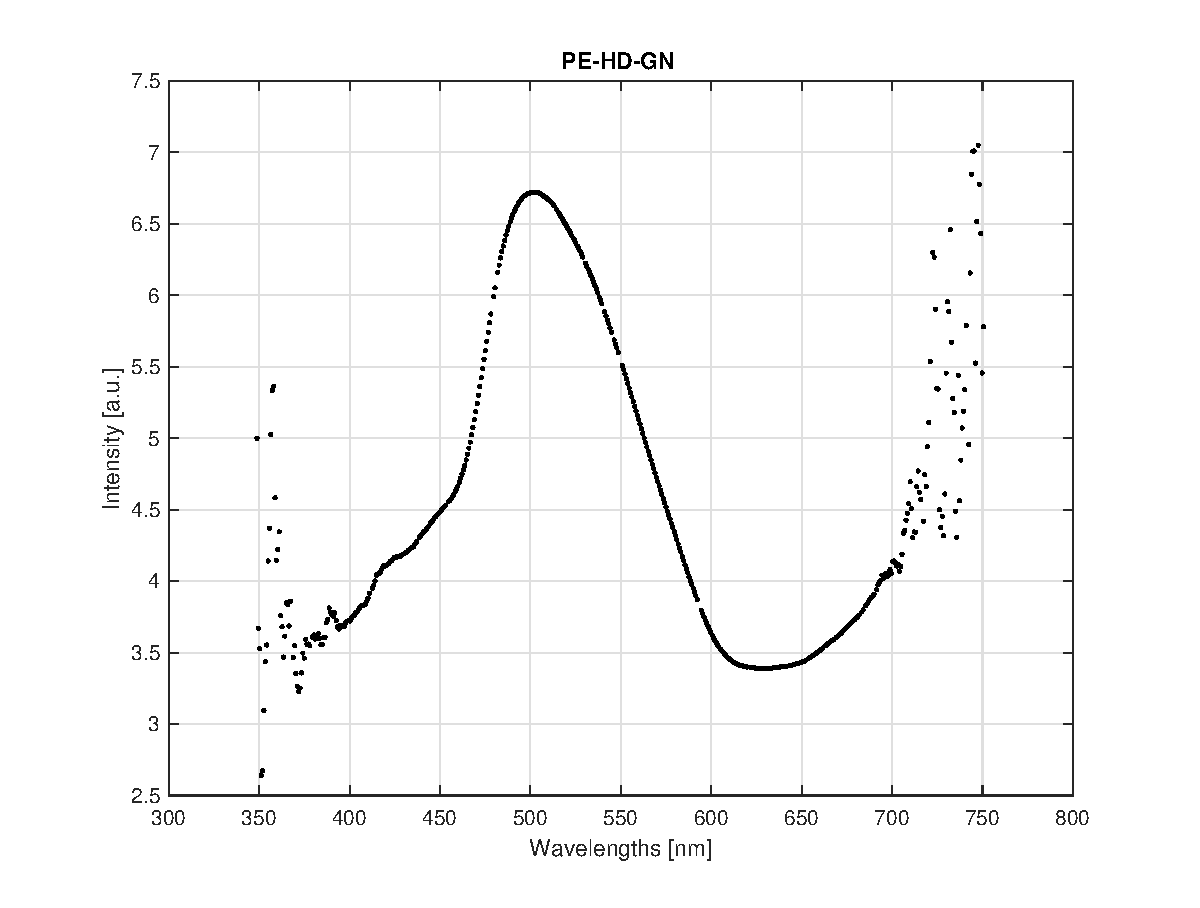
\includegraphics[scale=0.36]{Images/appendix/pe-hd-postconsumer-green.eps}}
  \begin{minipage}{\wd\FigBox}
    \centering\usebox{\FigBox}
    \subcaption{a) PE-HD Post Consumer, Green}
  \end{minipage}
  % Save second image 
  % Top image is centered, so no need to get width
 \sbox{\FigBox}{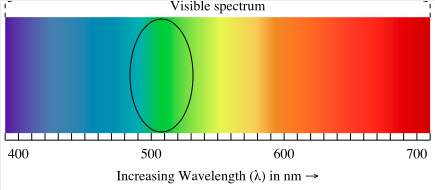
\includegraphics[scale=0.4]{Images/results/specgreen.png}}
  \begin{minipage}{\wd\FigBox}
    \centering\usebox{\FigBox}
    \subcaption{b) The visible light spectrum, circled at green}
  \end{minipage}
  \caption{A comparison of the resulting signature for green-colored PE-HD and the visible light spectrum-reference}
  \label{fig:green}
\end{figure}

%red
\begin{figure}[H]
  \newcommand*\FigVSkip{0.5em}
  \newcommand*\FigHSkip{0.1em}
  \newsavebox\FigBox
  \centering
  % Top image is centered, so no need to get width
 \sbox{\FigBox}{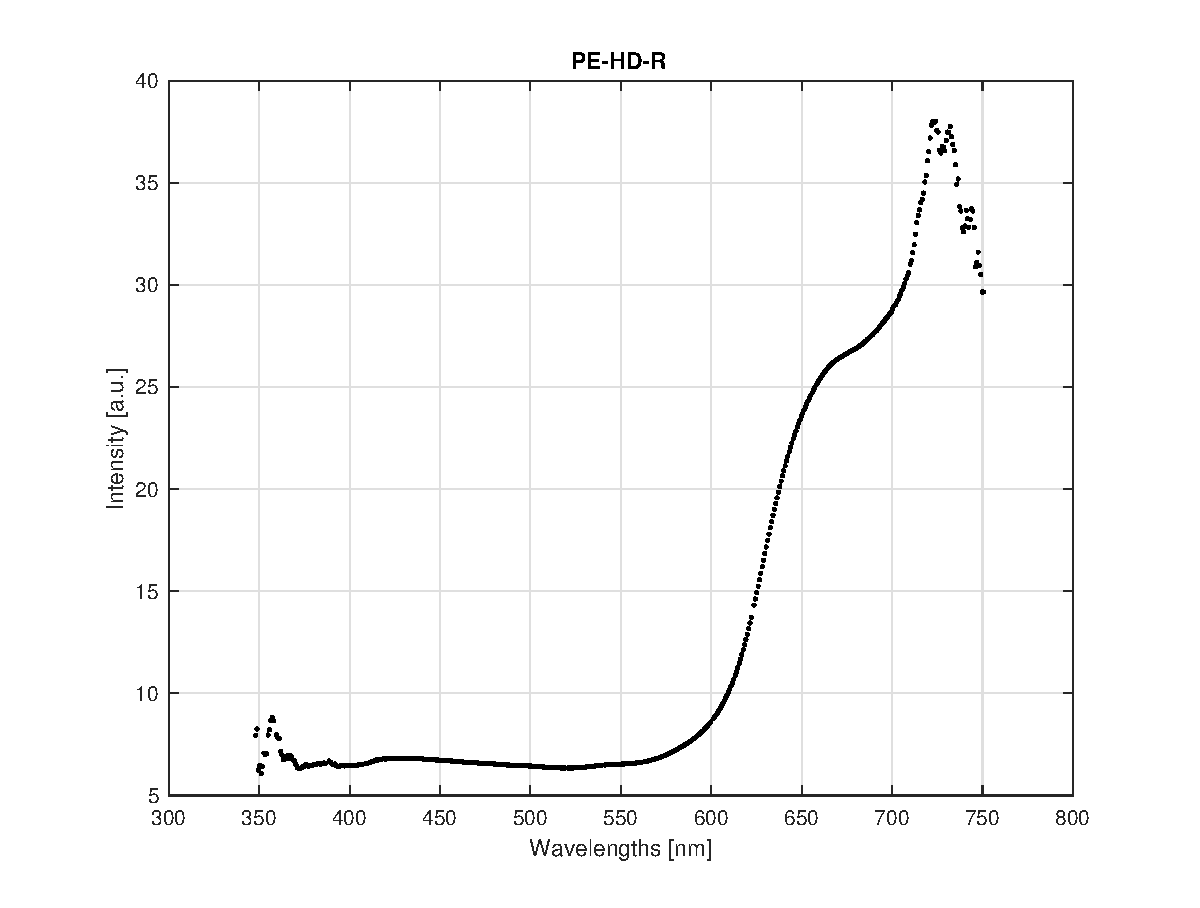
\includegraphics[scale=0.36]{Images/appendix/pe-hd-postconsum-red.eps}}
  \begin{minipage}{\wd\FigBox}
    \centering\usebox{\FigBox}
    \subcaption{a) PE-HD Post Consumer, Red}
  \end{minipage}
    % Top image is centered, so no need to get width
 \sbox{\FigBox}{\includegraphics[scale=0.4]{Images/results/specred.png}}
  \begin{minipage}{\wd\FigBox}
    \centering\usebox{\FigBox}
    \subcaption{b) The visible light spectrum, circled at red}
  \end{minipage}
  % Save second image 
  \caption{A comparison of the resulting signature for red-colored PE-HD and the visible light spectrum-reference}
  \label{fig:red}
\end{figure}

%blue
\begin{figure}[H]
  \newcommand*\FigVSkip{0.5em}
  \newcommand*\FigHSkip{0.1em}
  \newsavebox\FigBox
  \centering
  % Top image is centered, so no need to get width
 \sbox{\FigBox}{\includegraphics[scale=0.36]{Images/appendix/pe-ld-postindust-blue.eps}}
  \begin{minipage}{\wd\FigBox}
    \centering\usebox{\FigBox}
    \subcaption{a) PE-LD Post Industrial, Blue}
  \end{minipage}
    % Top image is centered, so no need to get width
 \sbox{\FigBox}{\includegraphics[scale=0.4]{Images/results/specblue.png}}
  \begin{minipage}{\wd\FigBox}
    \centering\usebox{\FigBox}
    \subcaption{b) The visible light spectrum, circled at blue}
  \end{minipage}
  % Save second image 
  \caption{A comparison of the resulting signature for blue-colored PE-LD and the visible light spectrum-reference}
  \label{fig:blue}
\end{figure}

%kilde for visible light reference
%https://www.khanacademy.org/science/physics/light-waves/introduction-to-light-waves/a/light-and-the-electromagnetic-spectrum

\noindent
This result support the earlier assertion about the color being dominant when detecting the spectral image of the plastic. Figures \ref{fig:green} and \ref{fig:red} are even the result of the same type of plastic, PE-HD. However, there is not much resemblance in the plots.
\\\\
The color variation is also found from the PCA as the second principal component. It is therefore reasonable to conclude that the specific color has a large influence.
\\\\
\subsection{Various Sizes}
Another interesting comparison is the result of the same type of plastic, in different sizes. In this section, illustrated by Figure \ref{fig:size}, a clear empty bottle of Farris, existent of PET-plastic, is compared to clear PET Amorphous. The pieces of PET Amorphous are 3mm thick, while the piece from the bottle is significantly larger. 

\begin{figure}[H]
  \newcommand*\FigVSkip{0.5em}
  \newcommand*\FigHSkip{0.1em}
  \newsavebox\FigBox
  \centering
  % Top image is centered, so no need to get width
 \sbox{\FigBox}{\includegraphics[scale=0.36]{Images/appendix/farris.eps}}
  \begin{minipage}{\wd\FigBox}
    \centering\usebox{\FigBox}
    \subcaption{a) Clear Farris Bottle}
  \end{minipage}
    % Top image is centered, so no need to get width
 \sbox{\FigBox}{\includegraphics[scale=0.36]{Images/appendix/pet-amorphous-pristine-clear.eps}}
  \begin{minipage}{\wd\FigBox}
    \centering\usebox{\FigBox}
    \subcaption{b) Clear PET Amorphous}
  \end{minipage}
  % Save second image 
  \caption{A comparison of a large PET piece from a Farris bottle and tiny PET Amorphous pieces}
  \label{fig:size}
\end{figure}
\noindent
When comparing the resulting signatures above, it is clear that they share trends. A quick look at Figure \ref{fig:size} reveals many similarities. Nevertheless, looking at the y-axis displaying intensity, one can observe a tripled intensity from the microplastic. 





\section{Discussion}
\label{sec:discussion}
 In this chapter several aspects of the project thesis will be discussed.
 
 %Klassifisering basert på PCA-resultatene
 

 
 
 
\section{Signatures Directly Interpreted}
In order to obtain a color-free spectrum, one could subtract the color spectrum from the resulting spectrum retrieved from the experiments. However, most pieces of plastic do not have one specific color, making it difficult to determine the spectrum to subtract. 
\\\\
In addition, when experimenting with different types of plastics having more or less the same colors, the results turned out next to identical. At first, a thought was that this was due to the color being too dominant in relation to the rest of the properties. However, conducting the same experiment with non-colored pieces of plastic, gave the same end-result; no difference in spectral signature even if the types of plastics differ. - could this be due to reflectance disturbance from "shiny" see through material, or is it in fact impossible to distinguish the different types from each other using hyperspectral imaging in visible light?
\\\\
Discussing the size-difference. Also, why is the intensity this different?
 
\section{Sources of Error}
Due to the ambient environment and sensors related to Hyper Spectral Imaging noise will be next to impossible to exclude. There is always some dark noise due to the sensors of the system. Also, since the measured values are based of a ratio rather than absolute values small changes could have large outcomes due to the fact that the values are divided by extremely small values. A change in the divisor may be small, but the outcome large due to the relative change. However, the tests were limited to the visible spectrum, whereas the biggest variation were in the infrared or near-infrared spectrum. Even though there were variations in the visible spectrum the results were satisfactory with respect to change due to noise. 
\\\\
Furthermore, the ambient light in the room is hard to completely avoid. Even though all light was turned off and blinds were used some light still got in. The light will affect the results, and could possibly affect the signature. However, due to the low amount of lighting that were present during the tests, it is assumed that it did not have a considerable effect on the results. The ambient light is therefore assumed to be negligible. 
\\\\
Even though the plastic was order specially in order to have pure samples, there are still sources that are unknown. As a result, the results could be affected by the differences in the plastic composition made by the manufacturer. However, the results showed a clear tendency where the actual color of the plastic was dominant as opposed to the chemical composition.
\\\\
The see-through plastic will be affected by the background. Compensating for the paper was not performed, and the results were most likely is affected by the background. The effect is not completely clear, but the trend of see through plastic have a similar peak to paper is could display the effect of the background. On the other hand, the background would most likely affect the results of the clear plastic either way. Therefore, the results were deemed satisfactory with the white background.
\\\\
The scanning was easily affected by the movement of the scanner. This was portrayed in the change of the reflectance standard. It is therefore a concern that the same effect will have caused the signatures to be inconsistent. However, the reflectance was regularly updated and there was several measurements per plastic type in order to account for large individual variations. It is still a concern that single measurements that were affected could skew the results.
\\\\


\section{Nothing but thoughts for now..}
VISUAL LIGHT:
Experiments analyzing the wave spectra of different types of plastics, have already been conducted. However, the results have been directed towards viewing the wave length interval describing near infrared light (NIR). Although the use of infrared light is an effective means of unobtrusive observation on land, it is far less effective in the ocean because long wavelength light is rapidly attenuated by seawater. One can therefore discuss whether it is possible to detect microplastic underwater with NIR. Is it possible to get close enough? etc..
\\\\
%https://oceanoptics.com/plastic-recycling-nir-spectroscopy/
Another important observation in these experiments, is the condition of the microplastic used. The material is pure and white, making the results independent of color. 
\\\\
%Water absorption 
%https://commons.wikimedia.org/wiki/File:Absorption_spectrum_of_liquid_water.png
%This logarithmic (log-log) graph shows water’s absorption behavior at different colors wavelength. As seen in the graph, water absorption is minimized between 400 -600 nm


%Light Transmission in the Ocean: http://www.waterencyclopedia.com/La-Mi/Light-Transmission-in-the-Ocean.html
%https://manoa.hawaii.edu/exploringourfluidearth/physical/ocean-depths/light-ocean

\\\\
\noindent
AN IDEA: 
What if we could inspect the level of additive acceptance in the different types of plastic. By finding the most resistant types, it might be possible to modify these into doing the same job as the types accepting additives. This way, we could reduce the production of the largest vectors/toxin-carriers. 

\todo[inline, color = red!60]{geir snakker om florescence of ditto lyssetting}
\chapter{Discussion}
\label{chap:discussion}
 In this chapter several aspects of the project thesis will be discussed.
 
 %Klassifisering basert på PCA-resultatene

VISUAL LIGHT
Experiments analyzing the wave spectra of different types of plastics, have already been conducted. However, the results has been directed towards viewing the wave length interval describing near infrared light (NIR). Although the use of infrared light is an effective means of unobtrusive observation on land, it is far less effective in the ocean because long wavelength light is rapidly attenuated by seawater.

%https://oceanoptics.com/plastic-recycling-nir-spectroscopy/
Another important observation in these experiments, is the condition of the microplastic used. The material is pure and white, making the results independent of color. 

Water absorption 
%https://commons.wikimedia.org/wiki/File:Absorption_spectrum_of_liquid_water.png
This logarithmic (log-log) graph shows water’s absorption behavior at different colors wavelength. As seen in the graph, water absorption is minimized between 400 -600 nm


Light Transmission in the Ocean: http://www.waterencyclopedia.com/La-Mi/Light-Transmission-in-the-Ocean.html
https://manoa.hawaii.edu/exploringourfluidearth/physical/ocean-depths/light-ocean


AN IDEA:
In order to obtain a color-free spectrum, one could subtract the color spectrum from the resulting spectrum retrieved from the experiments. However, most pieces of plastic do not have one specific color, making it difficult to determine the spectrum to subtract. 

In addition. When experimenting with different types of plastics having more or less the same colors, the results turned out next to identical. At first, a thought was that this was due to the color being too dominant in relation to the rest of the properties. However, conducting the same experiment with non-colored pieces of plastic, gave the same end-result; no difference in spectral signature even if the types of plastics differ. - this could also be due to reflectance disturbance from "shiny" see through material. 

ANOTHER IDEA: 
What if we could inspect the level of additive acceptance in the different types of plastic. By finding the most resistant types, it might be possible to modify these into doing the same job as the types accepting additives. This way, we could reduce the production of the largest vectors/toxin-carriers. 
\chapter{Conclusion and Further Work}
\label{chap:conclusion}
\section{Conclusion}
In this project thesis the aim was to do the necessary preparations for a master thesis that will be written and delivered in the spring of 2019. The research question asked at the beginning of this thesis was... Throughout experimental work and analysis, the answer has revealed itself. 
....
The results from the Principal Component Analysis of the measurements showed no clear clusters or trends that would make it possible to distinguish individual types of plastic at this stage. As PC1 represents the latent variable lightness and PC2 the latent variable color, the resulting correlation and variation in the set was not due to IOP from material composition..


\section{Further Work}
The further work on this project will be to complete the master thesis. 





\ifthenelse{\boolean{HarvardCitations}}{%
	\bibliographystyle{agsm} % used for Harvard style references. Names - Humanities & Interaction Design
}{%
	\bibliographystyle{ntnuthesis/ntnuthesis} %used for Vancover style references. Numbers - Computer Science & Physics
}

\bibliography{MastersExample}
\begin{appendices}

\chapter{Experiment Set-Up}
\label{app:method}


\chapter{PCA Results}
\label{app:PCA_res_full}

\chapter{List of Tested Plastic}
\label{app:list_plast}




\begin{figure}
    \centering
    \includegraphics[height = 9cm, angle = 90]{Images/order.png}
    \caption{List of microplastics - state, class, additives and application}
    \label{fig:order}
\end{figure}




\begin{comment}
\begin{center}
\begin{adjustbox}{angle=90}
\begin{tabular}{ |c|l|l|l|l| } 
 \hline
 \textbf{Ref Number} & \textbf{State} & \textbf{Class} & \textbf{Additives} & \textbf{Application}\\ 
 \hline
CRT131.00 & Post-Industrial Recyclate Pellets & PE: LDPE/LLDPE & Colorants, Printing inks & Extrusion, sheet\\
CRT150.00 & Post-Consumer Recyclate Regrind & PE-HD & Colorants & Injection moulding, crates\\
CRT170.00 & Environmental Pellets & PE: LDPE/HDPE & Unspecified Additives & Waste, beached pellets\\
CRT171.00 & Environmental Fragments (Regrind) & PE-HD & Unspecified Additives & Waste, beached fish box yellow\\
CRT200.00 & Pristine Pellets & PP-Homopolymer & Stabilizers & Extrusion, injection moulding\\
CRT250.00 & Post Consumer Recyclate: Pellets & PP Mixture & Unspecified Additives & Mainly Injection Moulding\\
CRT300.00 & Pristine Pellets & PS General purpose & Unknown & Extrusion blending, packaging\\
CRT331.00 & Post Consumer Recyclate Regrind & PS Mixture & Unspecified Additives & Plant Trays Outdoor\\ 
CRT400.00 & Pristine Pellets & PET Amorphous & No intentionally additives & Blow moulding \& extrusion sheet\\
CRT451.00 & Post Consumer Recyclate Regrind & PET Amorphous & No intentionally additives & Blow moulding \& extrusion sheet\\
CRT500.00 & Pellets & PVC Soft & Softener & Injection moulding \& extrusion\\
CRT530.00 & Pellets & PVC Hard & Softener \& Mineral Filler & Injection moulding \& extrusion\\
 \hline
\end{tabular}
\end{adjustbox}
\end{center}
\end{comment}

\chapter{Images of Tested Plastic Samples}
\label{app:image_plast}


\chapter{Plots of Signatures}
\label{app:signatures}

\begin{figure}
    \centering
    \includegraphics[width = 12cm]{Images/appendix/All.eps}
    \caption{All}
    \label{fig:all}
\end{figure}

\begin{figure}
    \centering
    \includegraphics[width = 12cm]{Images/appendix/farris.eps}
    \caption{Farris}
    \label{fig:my_label}
\end{figure}

%DENNE FUNKER IKKE!?!
\begin{comment}
\begin{figure}
    \centering
    \includegraphics[width = 12cm]{Images/appendix/isklar(blue).eps}
    \caption{Isklar}
    \label{fig:isklar}
\end{figure}
\end{comment}

\begin{figure}
    \centering
    \includegraphics[width = 12cm]{Images/appendix/p-env_yellowbowl.eps}
    \caption{PE environmental (yellow fishbowl)}
    \label{fig:pe_env}
\end{figure}

\begin{figure}
    \centering
    \includegraphics[width = 12cm]{Images/appendix/papersheet.eps}
    \caption{Paper sheet}
    \label{fig:paper}
\end{figure}

\begin{figure}
    \centering
    \includegraphics[width = 12cm]{Images/appendix/pe-beach-black.eps}
    \caption{PE beach-pellets, black}
    \label{fig:pe_beach_b}
\end{figure}

\begin{figure}
    \centering
    \includegraphics[width = 12cm]{Images/appendix/pe-beach-white.eps}
    \caption{PE beach-pellets, white}
    \label{fig:pe_beach_w}
\end{figure}

\begin{figure}
    \centering
    \includegraphics[width = 12cm]{Images/appendix/pe-hd-postconsum-gray.eps}
    \caption{PE-HD, Post Consumer, Gray}
    \label{fig:pehd-gray}
\end{figure}

\begin{figure}
    \centering
    \includegraphics[width = 12cm]{Images/appendix/pe-hd-postconsum-red.eps}
    \caption{PE-HD, Post Consumer, Red}
    \label{fig:pehd-red}
\end{figure}

\begin{figure}
    \centering
    \includegraphics[width = 12cm]{Images/appendix/pe-hd-postconsum.eps}
    \caption{PE-HD, Post Consumer, Yellow}
    \label{fig:pehd-yellow}
\end{figure}

\begin{figure}
    \centering
    \includegraphics[width = 12cm]{Images/appendix/pe-hd-postconsumer-green.eps}
    \caption{PE-HD, Post Consumer, Green}
    \label{fig:pehd-green}
\end{figure}

\begin{figure}
    \centering
    \includegraphics[width = 12cm]{Images/appendix/pe-ld-postindust-blue.eps}
    \caption{PE-LD, Post Industrial, Blue}
    \label{fig:peld-blue}
\end{figure}

\begin{figure}
    \centering
    \includegraphics[width = 12cm]{Images/appendix/pe-ld-postindust-gray.eps}
    \caption{PE-LD, Post Industrial, Gray}
    \label{fig:peld-gray}
\end{figure}

\begin{figure}
    \centering
    \includegraphics[width = 12cm]{Images/appendix/pe-ld-postindust-green.eps}
    \caption{PE-LD, Post Industrial, Green}
    \label{fig:peld-green}
\end{figure}

\begin{figure}
    \centering
    \includegraphics[width = 12cm]{Images/appendix/pepsi.eps}
    \caption{Pepsi}
    \label{fig:pepsi}
\end{figure}

\begin{figure}
    \centering
    \includegraphics[width = 12cm]{Images/appendix/pet-amorphous-pristine-clear.eps}
    \caption{PET Amorphous, Clear}
    \label{fig:pet}
\end{figure}

\begin{figure}
    \centering
    \includegraphics[width = 12cm]{Images/appendix/pet-postconsum.eps}
    \caption{PET Post Consumer, Clear}
    \label{fig:pet-pc}
\end{figure}

\begin{figure}
    \centering
    \includegraphics[width = 12cm]{Images/appendix/pp-postconsum-gray.eps}
    \caption{PP, Post Consumer, Gray}
    \label{fig:pp-gray}
\end{figure}

\begin{figure}
    \centering
    \includegraphics[width = 12cm]{Images/appendix/pp-pristine-clear.eps}
    \caption{PP, Pristine, Clear}
    \label{fig:pp-clear}
\end{figure}

\begin{figure}
    \centering
    \includegraphics[width = 12cm]{Images/appendix/ps-pristine-clear.eps}
    \caption{PS, Pristine, Clear}
    \label{fig:ps-clear}
\end{figure}

\begin{figure}
    \centering
    \includegraphics[width = 12cm]{Images/appendix/ps-postindust.eps}
    \caption{PS, Post Industrial, Looks like black/orange/white coffee powder}
    \label{fig:ps-coffee}
\end{figure}

\begin{figure}
    \centering
    \includegraphics[width = 12cm]{Images/appendix/pvc-pristine-colored.eps}
    \caption{PVC, Pristine, Gray}
    \label{fig:pvc-gray}
\end{figure}

\begin{figure}
    \centering
    \includegraphics[width = 12cm]{Images/appendix/pvc-soft-pristine-clear.eps}
    \caption{PVC Soft, Pristine, Clear}
    \label{fig:pvc-clear}
\end{figure}

\begin{figure}
    \centering
    \includegraphics[width = 12cm]{Images/appendix/remablue.eps}
    \caption{REMA Bag, Blue}
    \label{fig:remablue}
\end{figure}

\begin{figure}
    \centering
    \includegraphics[width = 12cm]{Images/appendix/remared.eps}
    \caption{REMA Bag, Red}
    \label{fig:remared}
\end{figure}

\begin{figure}
    \centering
    \includegraphics[width = 12cm]{Images/appendix/remawhite.eps}
    \caption{REMA Bag, White}
    \label{fig:remawhite}
\end{figure}

\begin{figure}
    \centering
    \includegraphics[width = 12cm]{Images/appendix/vinmono.eps}
    \caption{Vinmonopolet Bag, Black}
    \label{fig:vinmono}
\end{figure}





\end{appendices}






%\appendix
%\chapter{Appendix A}
\section{Curvature for the Global Model}





%\include{inc/timetable}

\end{document}
